\documentclass{report}
\usepackage[utf8]{inputenc}
\usepackage[a4paper, margin=2.5cm]{geometry}
\usepackage{graphicx}
% \usepackage[french]{babel}

% \usepackage[default,scale=0.95]{opensans}
\usepackage[T1]{fontenc}
\usepackage{amssymb} %math
\usepackage{amsmath}
\usepackage{amsthm}
\usepackage{systeme}
\usepackage{bbm}
\usepackage{hyperref}
\usepackage{tkz-tab}
\usepackage{latex_sty/Boites}

\usepackage{tikz}
\usepackage{xkeyval}

\hypersetup{
    colorlinks=true,
    linkcolor=blue,
    filecolor=magenta,      
    urlcolor=cyan,
    pdftitle={Optimisation Stochastique},
    % pdfpagemode=FullScreen,
    }
\urlstyle{same} %\href{url}{Text}

% \usepackage{mdframed}
\theoremstyle{plain} % default
% \newtheorem{thm}{Théorème}[section]
% \newtheorem{lem}[thm]{Lemme}
% \newtheorem{prop}[thm]{Proposition}
\newboxedtheorem[boxcolor=red, background=red!5, titlebackground=red!20, titleboxcolor = black]{thm}{Theorem}{thcounter}
\newboxedtheorem[boxcolor=red, background=red!5, titlebackground=red!20, titleboxcolor = black]{prop}{Proposition}{thcounter}
\newboxedtheorem[boxcolor=red, background=red!5, titlebackground=red!20, titleboxcolor = black]{lem}{Lemma}{thcounter}
\newtheorem*{cor}{Corollaire}
%\newtheorem*{KL}{Klein’s Lemma}

\theoremstyle{definition}
% \newtheorem{defn}{Définition}[section]
\newboxedtheorem[boxcolor=green, background=green!5, titlebackground=green!20, titleboxcolor = black]{defn}{Définition}{thcounter}
% \newtheorem{exmp}{Exemple}[section]
\newboxedtheorem[boxcolor=gray, background=gray!5, titlebackground=gray!20, titleboxcolor = black]{exmp}{Exemple}{thcounter}
% \newtheorem{xca}[exmp]{Exercise}

\theoremstyle{remark}
\newtheorem*{rem}{Remarque}
\newtheorem*{note}{Note}
\newtheorem{case}{Case}

\newcommand{\ind}{\perp\!\!\!\!\perp} 
\NewDocumentCommand{\underarrow}{O{=} O{\downarrow} m}{%
  \underset{\makebox[0pt]{\begin{tabular}{@{}c@{}}\ensuremath{#2}\\[0pt]#3\end{tabular}}}{#1}
}
\NewDocumentCommand{\overarrow}{O{=} O{\uparrow} m}{%
  \overset{\makebox[0pt]{\begin{tabular}{@{}c@{}}#3\\[0pt]\ensuremath{#2}\end{tabular}}}{#1}
}

\title{Optimisation Stochastique}
\author{Charles Vin}
\date{S1-2023}

\begin{document}
\maketitle

%RATRAPER COURS 1 
\chapter{Some basics of statistical learning}

\underline{Nouveau cours du 15/11} 

$\mathcal{D}_n = {(X_1, Y_1), \dots, (X_n,Y_n)}$ training samples iid copies of $(X,Y)$. $X \in \mathcal{X}$ and $Y \in \mathcal{Y}$ 

\begin{itemize}
    \item \textbf{goal} : fing a predictor surch that $f(X_i) \simeq Y_i$ on the training set. \\
    but above all $f(X_{\text{new}}) \simeq Y_{\text{new}}$ (test set) 
    \item \textbf{Risk} : $\mathcal{R}^{\textcolor{green}{(l)} }(f) = \underarrow[\mathbb{E}][\uparrow]{\textcolor{red}{on (X,Y)}} [ \overarrow[\ell][\downarrow]{\textcolor{green}{loss}}(Y, f(X))]$
    \item \textbf{Bayes predictor} : $f^\ast  \in \arg \min \mathcal{R}(f)$ \\
    $ \mathcal{R}^\ast = \mathcal{R}(f^\ast) = \inf \limits_{f} \mathcal{R}(f) $
    \item \textbf{Empirical risk} : $\hat{\mathcal{R}}_n (f) := \frac{1}{n} \sum \limits_{i=1}^{n} \ell (Y_i, f(X_i))$ \\
    $\hat{f}^{\text{ERM}} \in  \arg \min \limits_f \hat{\mathcal{R}}_n (f) $ (On some class of predictor)
\end{itemize}

Statistical learning theory focuses on controlling 
\[
    \mathcal{R}_n (\hat{f}_n) - \mathcal{R}^\ast  \text{  or  } \hat{\mathcal{R}}_n (\hat{f}_n) - \mathcal{R}^\ast
\]
for $\hat{f}_n$ a constructed predictor on the training set of size $n$. \\

\textbf{Classical error decomposition} :
\[
    \mathcal{R} (\hat{f}_n) - \mathcal{R}^\ast = 
    \textcolor{violet}{\underbrace{\color{black}\inf_{f \in \mathcal{F}} \mathcal{R}(f) - \mathcal{R}^\ast }_{\text{approximation error}} } 
    + \textcolor{cyan}{\underbrace{\color{black} \mathcal{R}(\hat{f}^\text{ERM}) - \inf_{f \in \mathcal{F}} \mathcal{R}(f) }_{\text{estimation error}} }
    +  \textcolor{gray}{\underbrace{\color{black} \mathcal{R} (\hat{f}_n) - \mathcal{R}(\hat{f}^\text{ERM}) }_{\substack{\text{error due to the use of an} \\ \text{ optimisation algo for ERM} } }}
.\]


%\begin{wrapfigure}{r}{0.4\textwidth}
%    \centering
%    \vfill
%    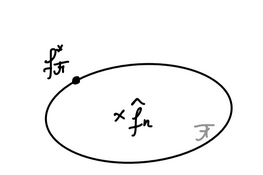
\includegraphics[width=0.35\textwidth]{figs/overfitting_ERM.png}
%    \caption{Overfitting for ERM}
%    \vfill  
%\end{wrapfigure} 

\begin{figure}[h]
    \begin{minipage}{0.5\textwidth}
        \textbf{Control of the estimation error} \\
        "Overfitting" : we have 
        \[
            \textcolor{gray}{\underbrace{\color{black} \hat{\mathcal{R}}_n (\hat{f}_n) }_{\text{train risk}  }}
            <<<
            \textcolor{gray}{\underbrace{\color{black} \mathcal{R}_n (\hat{f}_n) }_{\text{test risk}  }}
        .\]
    \end{minipage}
    \begin{minipage}{0.5\textwidth}
        \centering
        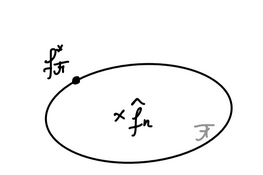
\includegraphics[width=0.8\textwidth]{figs/overfitting_ERM.png}
        \caption{Overfitting for ERM.}
        %\label{fig:figure}
    \end{minipage}
\end{figure}


\begin{lem}[]
    For the ERM predictor $\hat{f}_n = \hat{f}^{\text{ERM}}$, one has 
    \[
        \mathcal{R}(\hat{f}^{\text{ERM}}) - \mathcal{R}(f^\ast _{\mathcal{F}}) \leq 2 \sup_{f \in \mathcal{F}} \left| \hat{\mathcal{R}_n} - \mathcal{R} \right| (f)
    .\]
    with $f^\ast _{\mathcal{F}} \in \arg \min \limits_{f \in \mathcal{F}}\mathcal{R}(f)$
\end{lem}

Meaning the there is a link between estimation error and control of empirical process.

\begin{proof}[Preuve : ]
    \begin{align*}
        \mathcal{R} (\hat{f}^{\text{ERM}}) - \mathcal{R}(f^\ast _{\mathcal{F}}) 
        & = \textcolor{gray}{\underbrace{\color{black} \mathcal{R} (\hat{f}^{\text{ERM}}) \textcolor{blue}{-} \hat{\mathcal{R}}_n(\hat{f}^{\text{ERM}})}_{\leq \sup\limits_{f \in \mathcal{F}} ( \hat{\mathcal{R}_n} - \mathcal{R} ) (f) } }
        \textcolor{blue}{+} \textcolor{gray}{\underbrace{ \color{black} \hat{\mathcal{R}}_n(\hat{f}^{\text{ERM}}) \textcolor{red}{-} \hat{\mathcal{R}}_n(f^\ast_ \mathcal{F} ) }_{\leq 0 \text{ by optimality of } \hat{f}^{\text{ERM}} }}
        \textcolor{red}{+} \textcolor{gray}{\underbrace{ \color{black} \hat{\mathcal{R}}_n(f^\ast_ \mathcal{F} ) - \mathcal{R}(f^\ast _{\mathcal{F}}) }_{\leq \sup\limits_{f \in \mathcal{F}} ( \hat{\mathcal{R}_n} - \mathcal{R} ) (f) }} \\
        &\leq 2 \sup_{f \in \mathcal{F}} \left| \hat{\mathcal{R}_n} - \mathcal{R} \right| (f)
    \end{align*}
\end{proof}


Technics to control the supremum of empirical process.
\begin{itemize}
    \item In expectation : $\mathbb{E}[ \mathcal{R}(\hat{f}^\text{ERM}) - \mathcal{R}(f^\ast _{\mathcal{F}})]$ small? \\
    tool : Pisier's lemma
    \item in proba : $\mathbb{P}(\mathcal{R}(\hat{f}^\text{ERM}) - \mathcal{R}(f^\ast _{\mathcal{F}}) > \varepsilon ) \leq \delta $ \\
    tool : union bound + Hoeffding inequality
\end{itemize}

\begin{thm}[Hoeffding's inequality]
    $X_1, \dots X_n \ind$ r.v. and $X_i \in [a_i, b_i]$ a.s. \\
    then \begin{align*}
        \mathbb{P}(\left| \frac{1}{n} \sum_{i=1}^{n} (X_i - \mathbb{E}[X_i]) \right| > \varepsilon ) 
        & \leq 2 e^{-\dfrac{2 n ^2 \varepsilon ^2}{\sum_{i}^{} (b_i - a_i)^2}} \\
        \text{when} \begin{cases}
             &a_i =a\\
             &b_i =b\\
        \end{cases} \quad \rightarrow  & \leq  2 e^{-\dfrac{2 n \varepsilon ^2}{(b - a)^2}}
    \end{align*} 
\end{thm}

\begin{enumerate}
    \item When $n to + \infty $ ($\varepsilon $ fixed) the bound goes to 0.
    \item When $b -a \to + \infty $ the bound goes to 1.
    \item The R.H.S (right hand side) should depend on $\frac{\varepsilon }{b-a}$ (One could rescale $X_i$ by $\frac{1}{b-a}$ )
    \item By the CLT, the R.H.S should go to a constant if $n \to \infty $ and $\varepsilon = \frac{\tau }{\sqrt[]{n}}$ \begin{align*}
        \mathbb{P} ( \frac{1}{n} \sum_{i=1}^{n} (X_i &- \mathbb{E}[X_i]) >  \frac{\tau }{\sqrt[]{n}}) =  \mathbb{P}( \frac{1}{\sqrt{n}} \sum_{i=1}^{n} (X_i - \mathbb{E}[X_i]) >  \tau) \\
        & \xrightarrow[n \to \infty]{} \mathbb{P}(\mathcal{N}(0, . ) > \tau ) = \text{ constant }(\tau )
    \end{align*}
\end{enumerate}

\begin{prop}[]
    In the case of binary classification ($y = \{+1, -1\}$), concider a finite class $\mathcal{F}$ of predictors, i.e. of cardinality $\left| \mathcal{F} \right| < + \infty $. 
    \[
        \mathbb{P}(\sup _{f \in  \mathcal{F}} \left| \hat{\mathcal{R}}_n - \mathcal{R} \right|(f)> \varepsilon  ) \leq 2 \left| \mathcal{F} \right| e^{-2n \varepsilon^2} 
    .\]
\end{prop}

\begin{proof}[Preuve : ]
    \begin{align*}
        \mathbb{P}(\sup_{f in \mathcal{F}} \left| \hat{\mathcal{R}}_n - \mathcal{R} \right| (f) > \varepsilon  ) 
        &= \mathbb{P} ( \bigcup _{f \in \mathcal{F}} \{ \left| \hat{\mathcal{R}}_n - \mathcal{R} \right| (f) > \varepsilon \}) \\
        & \leq \sum_{f in \mathcal{F}}^{} \mathbb{P}(\left| \hat{\mathcal{R}}_n - \mathcal{R} \right| (f) > \varepsilon ) \qquad \text{[Union bound]}
    \end{align*}

    But $\left| \hat{\mathcal{R}}_n - \mathcal{R} \right| (f) = \frac{1}{n} \left| \sum_{i=1}^{n} \mathbbm{1}_{f(X_i) \neq Y_i} - \mathbb{E}[\mathbbm{1}_{f(X_i) \neq Y_i}] \right| = \frac{1}{n} \left| \sum_{i=1}^{n} Z_i - \mathbb{E}[Z_i] \right| $ \\
    with $Z_i \in \{0, 1\} \in [0,1]$ \\
    Therefore $\forall f \in  \mathcal{F}, \mathbb{P}(\left| \hat{\mathcal{R}}_n - \mathcal{R} \right| (f) > \varepsilon ) \leq 2 e^{-2n \varepsilon ^2}$. \\
    Finally, $$\mathbb{P}(\sup _{f \in  \mathcal{F}} \left| \hat{\mathcal{R}}_n - \mathcal{R} \right|(f)> \varepsilon  ) \leq 2 \left| \mathcal{F} \right| e^{-2n \varepsilon^2} $$
\end{proof}


\textcolor{red}{TO BE COMPLETED}

\underline{Nouveau cours du 16/11} \\

CCL du cours de la dernière fois 
\[
    R^\phi (\hat{h} ^{ \phi - \mathbb{E}R?}) - R^\phi (h ^\star , \phi )
.\]

\section{Relation between $ R^\phi  $ and $ R^{0/1} $  }
In this section, no empirical proof, no n
\begin{itemize}
    \item $ R^\phi(h) = \mathbb{E}[\phi (- Y h(X))]  $ 
    \item $ R^{0/1}(h) = \mathbb{E}[ \mathbbm{1}_{Y \neq sign(h(X))} ] $ 
    \item $ \phi  $ = hinge / logistic / least square
\end{itemize}

\begin{lem}[]
    If $ \phi  $ is diff, convex, increasing, then $ sign(h^{\star, \phi }) = f^{\star, Bayes} $ with $ h^{\star, \phi }  \in  \arg \min_h R^\phi (h)$ 
\end{lem}
\begin{proof}[Proof:]
    \begin{enumerate}
        \item \begin{align*}
            R^\phi (h) &= \mathbb{E}[\phi (-Yh(X))(\mathbbm{1}_{Y=1} + \mathbbm{1}_{Y = -1}) | X] \\ 
                &= \mathbb{E}[\phi (-h(X)) \eta (X) + \phi (h(X)) (1 - \eta (X))]
        \end{align*}
        with $ \eta (X) = P(Y=1 | X) $
        
        \item Define $ H_\phi (p, \eta ) := \eta \phi (-p) + (1 - \eta ) \phi (p) $ and $ p^{\star , \phi }(\eta ) = \arg \min H_\phi (p, \eta ) $ (assuming existence for now) \\
        $ h^{\star , \phi }  $ minimizes $ R^\phi  $  and is such that for any fixed $ x $ 
        \[
            h^{\star , \phi }(x) = p^{\star , \phi }(\eta (x))
        .\]
        $ \forall h, R^\phi (h) - R^\phi (h^{\star , \phi }) = \mathbb{E}[H_\phi (h(X), \eta (X)) - H_\phi (h^{\star , \phi }(X), \eta (X))] $ 
        
        \item Example for Least Square : \begin{align*}
            H_\phi (p, \eta ) &= \eta (1 - p)^2 + (1 - p)(1 + p)^2 \\
            \frac{\partial H_\phi }{\partial p} (p , \eta ) &= 2 (p -1) \eta + 2(1 - \eta )(1+p) \\
                    &= 0 \Leftrightarrow p = 2 \eta - 1
        \end{align*} 


        See Table \ref*{table:loss}
        
        In all cases, $ sign(p^{\star , \phi }(\eta (X)) = sign(\eta (X) - 1/2)) = sign(h^{\star , \phi }(X)) = f^{\star , Bayes}$ 

        \item In general with $ \phi  $ strictly increasing, diff, convex, when $ \phi (t) \to _{t \to +\infty } + \infty $  $ \forall \eta \in ]0, 1[, H_\phi (\eta , p) \to _{p \to  \pm \infty } + \infty $ . Thus $ p^{\star , \phi }(\eta ) $ exists. And $ p \mapsto H_\phi (p, \eta ) $ is diff 
        \[
            \frac{\partial H_{\phi }}{\partial p} (p , \eta ) = 0 \Leftrightarrow \eta \phi ' (-p^{\star , \phi }(\eta )) = (1 - \eta ) \phi (p^{\star , \phi } (\eta )) 
        .\]
        \begin{enumerate}
            \item If $ \eta < 1/2 $, then $ \eta < 1 - \eta \Rightarrow  \phi ' ( p^{\star , \phi } (\eta )) > \phi ' (p^{\star , \phi } (\eta )) \Rightarrow  p^{\star , \phi } ( \eta ) \leq 0$ 
            \item If $ \eta > 1/2 $ ... $ \Rightarrow p^{\star , \phi } \geq 0 $ 
        \end{enumerate}
    \end{enumerate}
    Finally, $ sign(p^{\star , \phi } ( \eta ) = sign( \eta - 1/2) ) $ and thus $ sign(h^{\star , \phi } (X) ) = f^{\star , Bayes } (X)$  

\end{proof}

\begin{table}[!ht]
    \centering
    \begin{tabular}{|l|l|l|}
    \hline
        Loss & $ p^{\star , \phi }(\eta ) $  & $ \min H_\phi (p, \eta ) $  \\ \hline
        LS : $ (1 + v)^2 $  & $ 2 \eta - 1 $  & $ 4 \eta (1 - \eta )  $  \\ \hline
        Hinge & sign & a \\ \hline
        Logistic & a & a \\ \hline
    \end{tabular}
    \label{table:loss}
\end{table}


\begin{lem}[Zhang]
    Assume $ phi $ increasing, convex such that $ \phi (0) = 1 $. For $ \gamma \geq 1 $ we have $ \left| \eta  - 1/2 \right|^\gamma  \geq c \left| 1 - H_\phi (p^{\star , \phi }(\eta ), \eta ) \right|   $ . \\
    $ \forall h $ classifier $ h: \mathcal{X} \to \mathbb{R} $ 
    \[
        R^{0/1} (sign(h)) - R^{0/1}(f^{\star , Bayes}) \leq 2 c ^{1/\gamma }(R^\phi (h) - R^\phi (h^{\star , \phi }))
    .\]
\end{lem}

When $ h $ approximately minimizes the relaxed excess risk its $ sign(h) $ behaves well in terms of the initial excess risk !!. 

\begin{note}[]
    Note that $ \gamma = 2 $  for the square loss and the logistic loss. And that $ \gamma = 1 $ for the hinge loss. \\
    (we do not care about $ c $ )
\end{note}

\begin{proof}[Proof:]
    \begin{align*}
        R^{0/1} (sign(h)) - R^{0/1}(f^{\star , Bayes }) &= \mathbb{E}[ \mathbbm{1}_{sign(h(X)) \neq  f^{\star , Bayes}(X) 2  \left| \eta (X) - 1/2 \right| }] \\
        \text{(jensen, (1) )} &\leq \mathbb{E}[ \mathbbm{1}_{sign(h(X)) \neq  f^{\star , Bayes}(X) 2^\gamma  \left| \eta (X) - 1/2 \right| ^\gamma }]^{1/\gamma } \\
                        &\leq 2 c^{1/\gamma } \mathbb{E}[\mathbbm{1}_{sign(h(X)) \neq  f^{\star , Bayes}(X) } (1 - H_ \phi (p^\star _\phi  (\eta (X)) , \eta (X))]^{1/\gamma} (\eta (X) = P (Y=1 | X))
    \end{align*}
    \begin{note}[]
        Note that when $ sign(h(X)) \neq sign(\eta (X) - 1/2) $, then $ H_\phi ^\prime ( h(X), \eta (X) ) > 1 $. Indeed, $ \eta \phi (-p) + (1 - \eta ) \phi (p) \geq \phi ( - \eta  p + (1 - \eta ) p) = \phi ((1 - 2 \eta ) p )$ because $ \phi  $ convex. And now $ \phi ((1 - 2 \eta ) p) \geq  \phi (0) = 1 $ because $ \phi  $ increasing $ \geq 0 $ when $ sign(p) \neq sign(\eta - 1/2) $ 
    \end{note}
    
    \begin{align*}
        (1) &\leq  2 c^{1/\gamma } ( \mathbb{E} [ H( h(X), \eta (X)) - H(p^{\star , \phi }(\eta (X)), \eta (X)) ])^{1/\gamma } \\ 
            &= 2c ^{1/\gamma } ( R^\phi (h) - R^\phi (h^{\star , \phi }) )^{1/\gamma }
    \end{align*}
    
\end{proof}

CCL : $ \forall \hat{h} $ 
\begin{align*}
    R^{0/1} ( sign(\hat{h}) ) - R^{0/1} (f^{\star , Bayes }) \leq c^{1/\gamma } ( R^\phi (\hat{h}) - R^\phi (h^{\star , \phi }))^{1/\gamma } \\
    R^\phi ( \hat{h} ) - R^\phi ( h^{\star , \phi } ) = R^\phi (\hat{h}) - R^\phi (h^{\star , \phi }_\mathcal{F} ) + R^\phi (h^{\star , \phi }_\mathcal{F}) - R^\phi ( h^{\star , \phi } ) 
\end{align*}
where \begin{itemize}
    \item $ h^{\star , \phi }_\mathcal{F} \in \arg \min R^\phi (h) $ 
    \item $ R^\phi (h^{\star , \phi }_\mathcal{F}) - R^\phi ( h^{\star , \phi } ) $  approx error
\end{itemize}



\begin{align*}
    R^phi (\hat{h}) - R^\phi (h^{\star , \phi }_\mathcal{F}) &= R^\phi (\hat{h}) - \hat{R}^\phi_n(\hat{h}) (\leq  \sup _\mathcal{F} \hat{R}_n - R^\phi ) \\
        &+ \hat{R}^\phi _n (\hat{h}) - \hat{R}^\phi _n (\hat{h}^{\phi ERM}) \text{("optim error")} \\
        &+ \hat{R}^\phi _n (\hat{h}^{\phi-ERM}) - \hat{R}^\phi _n (\hat{h}^{\star , \phi } _\mathcal{F}) (\leq 0) \\
        &+ \hat{R}^\phi _n (h^{\star , \phi } _\mathcal{F}) - R^\phi (h^{\star , \phi } _ \mathcal{F}) (\leq \sup _\mathcal{F} \hat{R}^\phi _n - R^\phi )
\end{align*}
\textbf{Since the estimation error typically scales in $ O(\frac{1}{\sqrt[]{n}}) $ , no need to reach the ERM using our optimization algo !!.}

\begin{note}[]
    When using Lipschitz fonctions, we obtain slow rates $ O(\frac{1}{\sqrt[]{n}}) $. Is there a path towards fast rates ? Let's take the example of the mean estimation. 
    \begin{enumerate}
        \item Method 1 : \begin{align*}
            \hat{\theta } &= \frac{1}{n} \sum_{i=1}^{n} Z_i = \arg \min_\theta \frac{1}{2n} \sum_{i=1}^{n} (Z_i - \theta )^2  \\
            \theta ^\star &= \arg \min \frac{1}{2}\mathbb{E}[ (\theta - Z) ^2] = \mathbb{E}[Z]
        \end{align*}
        From the developpement before on the estimation error 
        \[
            R(\hat{\theta }) - R(\theta ^\star ) = O( \frac{1}{\sqrt[]{n}})
        .\]
        
        \item Method 2 : Direct computation \begin{align*}
            &R (\theta ) = \frac{1}{2}\mathbb{E}[(\theta  - Z)^2] = \frac{1}{2}(\theta - \mathbb{E}[Z])^2 + \frac{1}{2}Var(Z) \\
            &\Rightarrow R(\hat{\theta }) - R(\theta ^\star ) = R(\hat{\theta }) ( R(\mathbb{E}[Z])) = \frac{1}{2}(\hat{\theta } - \mathbb{E} (Z))^2 (\text{conditionallty to } \mathcal{D}_n)\\
            &\mathbb{E}_{D_n} [     ] = \frac{1}{2} \mathbb{E}[(\frac{1}{n} \sum_{}^{} Z_i - \mathbb{E}[Z])^2 ] = \frac{1}{2 \mathbf{n}} Var(Z) ( \mathbf{n} \text{ is FAST RATE } O(\frac{1}{n}))
        \end{align*}
        Bound only for this specific $ \hat{\theta } $ and because I also have stong convexity. 
        
        In supervised learning, fast rates can be established for strongly convex function (in our relaxed risks)
    \end{enumerate}
\end{note}

\chapter{Basics of deterministic optimisation}

In ML, construct a predictor often boils down to minimize an empirical risk using iterative algorithms.

\section{First order method}

\subsection{Basics of convex analysis}
$ F: \mathbb{R}^d \to \mathbb{R} $ convex, diff, L-smooth (its gradient is L-Lipschitz). 
\begin{itemize}
    \item convexity (under chords) : $ F(\eta \theta + (1 - \eta ) \theta ^\prime ) \leq  \eta F(\theta ) + (1 - \eta ) F(\theta ^\prime ), \forall \theta , \theta ^\prime , \forall \eta  \in 
    [0, 1] $ 
    \item If we add diff (tangent lie below) we have $ F(\theta ^\prime ) \geq F(\theta ) + \langle  \nabla F(\theta ) , \theta ^\prime - \theta  \rangle ,  \forall \theta , \theta ^\prime $ 
    \item (increasing slopes) $ \langle \nabla F(\theta ) - \nabla F(\theta ^\prime ), \theta - \theta ^\prime \rangle \geq 0 $ ($ \nabla F $ is said to be a monotone operator )
    \item if we add $ \mathcal{C}^2 $ (curves upwards) $ \forall \theta , Hess_F (\theta ) \succeq 0 $ (SDP)
\end{itemize}

$ \mu \text{-strongly}$ convex, $ \mu > 0 $. 
\begin{itemize}
    \item convexity (\textbf{"well"} under chords) : $ F(\eta \theta + (1 - \eta ) \theta ^\prime ) \leq  \eta F(\theta ) + (1 - \eta ) F(\theta ^\prime ) - \frac{\eta (1 - \eta ) \mu }{2} \left\| \theta - \theta ^\prime  \right\| ^2 _2 , \forall \theta , \theta ^\prime , \forall \eta  \in 
    [0, 1] $ 
    \item If we add diff (tangent lie \textbf{"well"} below) we have $ F(\theta ^\prime ) \geq F(\theta ) + < \nabla F(\theta ) , \theta ^\prime - \theta  > + \frac{\mu }{2} \left\| \theta - \theta ^\prime  \right\|^2_2, \forall \theta , \theta ^\prime  $ 
    \item (\textbf{"well"}increasing slopes) $ \langle \nabla F(\theta ) - \nabla F(\theta ^\prime ), \theta - \theta ^\prime \rangle \geq 0 + \mu \left\| \theta - \theta ^\prime  \right\| _2 ^2  $
    \item if we add $ \mathcal{C}^2 $ (curves upwards) $ \forall \theta , Hess_F (\theta ) \succeq \mu Id $ (SDP)
\end{itemize}
Other definition:
\begin{itemize}
    \item $ F $ is $ \mu \text{-strongly} $ convex $ \forall \theta _0, \theta \mapsto F(\theta ) - \frac{\mu }{2} \left\| \theta  - \theta _0 \right\|^2 _2 $ is convex.
    \item L-Smooth : $ \forall \theta , \theta ^\prime, \left\| \nabla F(\theta ) - \nabla F(\theta ^\prime ) \right\| \leq  L \left\| \theta - \theta ^\prime  \right\| $ 
\end{itemize}

\begin{lem}[Descent lemma]
    Assume that $ F $  is L-Smooth. Therefore $ \forall \theta , \theta ^\prime \in  $ domain of $ F $ 
    \[
        F(\theta ^\prime ) \leq  F(\theta ) + \langle \nabla F(\theta ) , \theta ^\prime  - \theta \rangle + \frac{L}{2} \left\| \theta ^\prime  - \theta  \right\| 
    .\]
\end{lem}
\begin{proof}[Proof:]
    \begin{align*}
        F (\theta ^\prime ) 
            &= F(\theta ) + \int_{0}^{1} < \nabla F(\theta  + t(\theta ^\prime - \theta )), \theta ^\prime - \theta > dt \\
            &= F(\theta ) \mathbf{+} < \nabla F(\theta ), \theta ^\prime  - \theta > + \int_{0}^{1} < \nabla F(\theta  + t(\theta ^\prime - \theta )) \mathbf{-} \nabla F(\theta ), \theta ^\prime  - \theta > dt \\
            &\leq F(\theta ) \mathbf{+} \langle \nabla F(\theta ), \theta ^\prime  - \theta \rangle + \int_{0}^{1} \left\| \nabla F(\theta + t(\theta ^\prime  - \theta )) - \nabla F(\theta ) \right\| \left\| \theta  ^\prime - \theta  \right\| dt \\
            &\leq F(\theta ) \mathbf{+} \langle \nabla F(\theta ), \theta ^\prime  - \theta \rangle + \int_{0}^{1} t L \left\| \theta ^\prime  - \theta  \right\|^2 dt \\
            &\leq F(\theta ) \mathbf{+} \langle \nabla F(\theta ), \theta ^\prime  - \theta \rangle + \frac{1}{2} L \left\| \theta  ^\prime  - \theta  \right\| ^2 _2
    \end{align*}
\end{proof}

\paragraph*{Consequence of this quadratics upper bound }

\begin{enumerate}
    \item \begin{align*}
        F(\theta ) &\leq F(\theta ^\star ) + \langle \nabla F(\theta ^\star ) , \theta  - \theta ^\star \rangle + \frac{L}{2} \left\| \theta - \theta ^\star  \right\| ^2 \\
        F(\theta ) - F(\theta ^\star ) &\leq \frac{L}{2} \left\| \theta  - \theta ^\star  \right\| ^2 
    \end{align*}
    \item 
    \[
        \min_\theta  F(\theta ) \leq \min _\theta F(\theta ) + \langle \nabla F(\theta ), \theta ^\prime - \theta \rangle  + \frac{L}{2}\left\| \theta ^\prime - \theta  \right\| ^2
    .\]
    $ \min _\theta F(\theta ) + \langle \nabla F(\theta ), \theta ^\prime - \theta \rangle  + \frac{L}{2}\left\| \theta ^\prime - \theta  \right\| ^2 $  is reach for $ \theta ^\prime  = \theta - \frac{1}{L} \nabla F(\theta ) $ 
    \begin{align*}
        &\leq F(\theta ) + \langle \nabla F(\theta ), \theta  - \frac{1}{L} \nabla F(\theta ) - \theta  \rangle + \frac{L}{2} \left\| \theta  - \frac{1}{L} \nabla F(\theta ) - \theta  \right\| ^2 \\
        &= F(\theta ) - \frac{1}{2L} \left\| \nabla F(\theta ) \right\| ^2
    \end{align*}

    All in all, $ \forall \theta  $ 
    \[
        \frac{1}{2L} \left\| \nabla F(\theta ) \right\| ^2 \leq  F(\theta ) - F(\theta ^\star ) \leq  \frac{L}{2} \left\| \theta  - \theta ^\star  \right\| ^2
    .\]
\end{enumerate}

\begin{note}[]
    In what follows, we could easily extend the study to non-diff function by involving \textbf{subgradients}. 
    
    $ F: \mathbb{R}^D \mapsto \mathbb{R} $ A vector $ \eta  \in \mathbb{R}^d $ is a subgradient of $ F $ at $ \theta  $ if 
    \[
        \forall \theta ^\prime, F(\theta ^\prime ) \geq F(\theta ) + \langle \eta , \theta ^\prime - \theta \rangle
    .\]
    $ \partial F(\theta ) $ is the subdifferential of $ F $ at $ \theta  $ a,d gathers all the subgradients of $ F $ at $ 0 $ i.e. the direction of hyperplanes passing through $ (\theta , F(\theta )) $ but remaining below the graph of $ F $ 

    \begin{figure}[h]
        \centering
        \includegraphics*[width=.5\textwidth]{figs/subgradients.jpg}
        \caption{subgradients}
    \end{figure}

\end{note}


\subsection{Gradient algorithms}
$ \theta ^\star = \arg \min F $ assuming existence and uniqueness. 

\subsubsection{Gradient algo}
\begin{enumerate}
    \item Init $ \theta _0  \in \mathbb{R} ^d $
    \item $ \forall t \geq 0, \theta _{t+1} = \theta _t - \gamma _{t+1} \nabla F(\theta _t) $ with $ \gamma _{t+1} $ gradient steps / learning rates
\end{enumerate}
Choice of steps : 
\begin{itemize}
    \item Constant step sizes $ \gamma _t = \gamma , \forall t $ it may depend on the time horizons $ T: \forall t \in [0, 1], \gamma _t = \gamma (T) $ 
    \item Line search : optimal step size at each iteration. $ \gamma _{t} = \arg \min _{\gamma > 0} F(\theta _{t-1} - \gamma \nabla F(\theta _{t-1}))) $. You can forget about that case in online algo!
\end{itemize}

\subsubsection{Link with the gradient flow}
The iterates of Gradient Descent (GD, Euler, XVIIIe)
\[
    \theta _{t+1} = \theta _t - \gamma _t \nabla F(\theta _t)
.\]
can be rewrittent as 
\[
    \frac{\theta _{t+1} - \theta _t}{\gamma _t} = - \nabla F(\theta _t)
.\]
Make the step size $ \gamma _t $ shrink to $ 0 $, we obtain the ODE 
\[
    \frac{\partial \theta }{\partial t} (t) = - \nabla F(\theta (t))
.\]
This continuous version is called the Gradient Flow (GF). Thus GD is a discretization of GF (using finite differences).

$ \nabla F(\theta ) $ is orthogonal to $ \{\theta ^\prime : F(\theta ^\prime ) = F(\theta )\} $ (level set) so that $ \frac{\partial \theta }{\partial t} (t) = \theta (t) $ point inwards $ \{\theta ^\prime : F(\theta ^\prime ) \leq F(\theta ) \} $ which guarantees that $ F(\theta (t)) $ is decreasing. \\
Indeed $ \frac{\partial (F \circ \theta )}{\partial t}(t) = \langle \nabla F(\theta (t)), \dot{\theta }(t) \rangle = - \left\| \nabla F(\theta (t)) \right\| ^2  $ 

\begin{thm}[]
    For $ F $ an L-Smooth. for $ \gamma _t = \gamma , \forall t $ with $ \gamma < 2/L $ 
    \[
        F(\theta _t) - F(\theta ^\star ) \leq \frac{\left\| \theta _0 - \theta 
        ^\star  \right\| }{2 \gamma (1 - \frac{\gamma L}{2}) T }
    .\]
    For $ \gamma = \frac{1}{L} $ we have 
    \[
        F(\theta _t) - F(\theta ^\star ) \leq \frac{\left\| \theta _0 - \theta ^\star  \right\| }{2 \gamma (1 - \frac{\gamma L}{2}) T } = \frac{L \left\| \theta _0 - \theta ^\star  \right\| ^2}{T}
    .\]

    \begin{note}[]
        \begin{enumerate}
            \item This is a sublinear rate $ O(1/T) $
            \item Using a constant step size. \\
            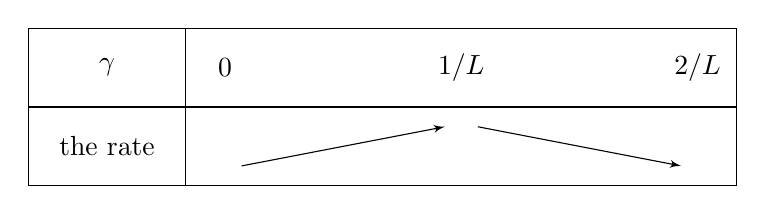
\begin{tikzpicture}
                \tkzTabInit{$\gamma $ / 1, the rate / 1}{ $0$, $1/L$, $2/L$ }
                \tkzTabVar{ -/, +/, -/}
             \end{tikzpicture}
            \item Optimal "constant" step size $ = \frac{1}{L} $ 
        \end{enumerate}
    \end{note}

    \begin{note}[Interpolation of GD with $ \gamma = \frac{1}{L} $ ]
        Note that \begin{align*}
            \tilde{\theta }_t 
                &= \arg \min F(\tilde{\theta }_{t-1}) + \langle \nabla F(\tilde{\theta } _{t-1}), \theta  - \tilde{\theta }_{t-1} \rangle + \frac{L}{2} \left\| \theta  - \tilde{\theta }_{t - 1} \right\| ^2 \\
                &= \tilde{\theta }_{t - 1} - \frac{1}{L} \nabla F(\tilde{\theta }_{t - 1})
        \end{align*}
        Using GD with $ \gamma = \frac{1}{L} $ amounts to minimizer a quadratic upper bound (provided by smoothness). This idea is a the heart of the Majorize-Minimize algo. 
    \end{note}
\end{thm}

\begin{proof}[Proof:]
    \begin{align*}
        \left\| \theta _{t+1} - \theta ^\star  \right\| ^2 _2  
            &\overset{(GD)}{=} \left\| \theta _t - \gamma \nabla F(\theta _t) - \theta ^\star  \right\| ^2 _2 \\
            &= \left\| \theta _t - \theta ^\star  \right\| ^2 _2 - 2 \gamma  \langle \nabla F(\theta _t), \theta _t - \theta ^\star \rangle + \gamma ^2 \left\| \nabla F(\theta _t) \right\| ^2 _2
    \end{align*}
    Function convex + L-Smooth : $ \left\| \nabla F(\theta ) \right\| ^2 \leq L \langle \nabla F(\theta ), \theta  - \theta ^\star \rangle $. This is a consequence of the co-coercivity of $ \nabla F $ (with param $ 1/L $ )
    \begin{note}[Co-coercivity]
        $ F $ convex, L-Smooth, then $ \theta , \theta ^\prime  $ 
        \[
            \langle  \nabla F(\theta ) - \nabla F(\theta ^\prime ), \theta  - \theta ^\prime \rangle \geq_{\text{co-coercivity}} \frac{1}{L} \left\| \nabla F(\theta ) - \nabla F(\theta ^\prime ) \right\| ^2 _2
        .\]
        \begin{proof}[Proof of the note on co-coercivity:]
            Define two function \begin{align*}
                G(\theta ^\prime ) &= F(\theta ^\prime ) - \langle \nabla F(\theta ) , \theta ^\prime \rangle  \\
                H(\theta ^\prime ) &= F(\theta ) - \langle \nabla F(\theta ^\prime ), \theta \rangle 
            \end{align*}
            $ G $ and $ H $ are smooth. $ \theta ^\prime = \theta  $ minimize $ \theta ^\prime  \mapsto G(\theta ^\prime ) $ and 
            \begin{align*}
                F(\theta ^\prime) - F(\theta ) - \langle \nabla F(\theta ) , \theta ^\prime - \theta  \rangle
                    &= G(\theta ^\prime) - G(\theta ) \\
                    &\geq \frac{1}{2L} \left\| \nabla G(\theta ^\prime ) \right\| ^2 (\text{by LHS, 1) and where "all in all"} ) \\
                    &= \frac{1}{2L} \left\| \nabla F(\theta ^\prime ) - \nabla F(\theta ) \right\| ^2
            \end{align*} 
            Idem, $ \theta  = \theta ^\prime  $ minimizes $ \theta \mapsto H(\theta ) $ 
            \begin{align*}
                F(\theta ) - F(\theta ^\prime ) - \langle \nabla F(\theta ^\prime ), \theta  - \theta ^\prime \rangle &= H (\theta ) - H(\theta ^\prime ) \\
                &\geq \frac{1}{2L} \left\| \nabla H(\theta )  \right\| ^2 \\
                &= \frac{1}{2L} \left\| \nabla F(\theta ^\prime ) - \nabla F(\theta ) \right\| ^2
            \end{align*}
            Sum the 2 inequalities to conclude
        \end{proof}
        End of the co-coercivity note
    \end{note}
    
    \begin{align*}
        \left\| \theta _{t+1} - \theta ^\star  \right\| ^2 
            &= \left\| \theta _t - \theta ^\star  \right\| ^2 - 2 \gamma  \langle \nabla F(\theta _t), \theta _t - \theta ^\star \rangle + \gamma  ^2 \left\| \nabla F(\theta _t) \right\| ^2 \\
            &\leq  \left\| \theta _t - \theta ^\star  \right\| ^2 - 2 \gamma ( 1 - \frac{\gamma L }{2}) \langle \nabla F(\theta _t) , \theta _t - \theta ^\star \rangle  \\
            &\Rightarrow 2 \gamma (1 - \frac{\gamma L}{2}) \langle \nabla F(\theta _t) , \theta _t - \theta ^\star \rangle \leq  \left\| \theta _{t-1} - \theta ^\star  \right\| ^2 - \left\| \theta _t - \theta ^\star  \right\| ^2  \\
            &\Rightarrow 2 \gamma (1 - \frac{\gamma L }{2}) (F(\theta _t) - F(\theta ^\star )) \leq  \left\| \theta _{t-1} - \theta ^\star  \right\| ^2 - \left\| \theta _t - \theta ^\star  \right\| ^2  \\
            &\Rightarrow F(\theta _t) - F(\theta ^\star )
            \leq \frac{1}{T}\sum_{t=1}^{T} F(\theta _t) - F(\theta ^\star ) \\
            &\leq \frac{\left\| \theta _0 - \theta ^\star  \right\| ^2}{ 2 \gamma (1 - \frac{\gamma L}{2}) T}
    \end{align*}
    
\end{proof}

\underline{Nouveau cours du 23/11} \\


RAPPEL : 
On regarde \begin{itemize}
    \item $ \theta _{t+1} = \theta _t - \gamma _t \nabla F(\theta _t)$ 
    \item $ \theta _0 \in \mathbb{R}^d $ 
\end{itemize}

\begin{thm}[]
    F L-smooth, diff \\
    For $\gamma_t = \gamma$ for all $t \leq0$
    
    \begin{align*}
        F(\theta _T) - F(\theta ^\infty ) 
            &\leq \frac{\left\| \theta _0 - \theta ^\infty \right\| ^2}{2 \gamma (1 - \frac{\gamma L}{2} )T} \\
            &= L \frac{\left\| \theta _0 - \theta ^\infty  \right\| ^2 }{T} (\gamma = 1/L)
    \end{align*}


    \begin{itemize}
        \item $\gamma = \dfrac{1}{L}$ It is the largest constant step size ensuring the most decrease of the objective fct at each iteration.
        \item L-smooth, diff $\mathcal{C}^2 \Leftrightarrow \lambda_{MAX}(H_F(\theta)) \leq L \forall \theta $
        \begin{align*}
            \Leftarrow  \left\| \nabla F(\theta ) - \nabla F(\theta ^\prime ) \right\|  
                &= \left\| \int_{0}^{1} H_F (\theta ^\prime + t ( \theta  - \theta ^\prime )) (\theta  - \theta ^\prime ) dt \right\| \\
                &\leq \int_{0}^{1} \left\| H_F (\theta  + t (\theta  - \theta ^\prime )) (\theta  - \theta ^\prime ) \right\| dt \\
                &\leq L \left\| \theta - \theta ^\prime  \right\| _2
        \end{align*}
    \end{itemize}
\end{thm}

\begin{thm}[]
    If $ F $ is L-Smooth, diff and $ \mu  $ - strongly convex, then for all step size $ \gamma \leq 1/L $ 
    \begin{align*}
        \left\| \theta _T - \theta ^\star  \right\| ^2 
            &\leq (1 - \gamma \mu ) ^T \left\| \theta _0 - \theta ^\star  \right\| ^2 \\
            (\text{for } \gamma = 1/L) &= (1 - \frac{\mu }{L}) ^T \left\| \theta _0 - \theta ^\star  \right\| ^2 (\text{for } \gamma = 1/L)
    \end{align*}
\end{thm}

\begin{note}
    \begin{enumerate}
        \item The algorithm is the same so the CV rate is improved only by properties of F. In such a case the rate is said to be linear.
        \item CV rate on the iterates (!!) and not only on the objective rate 
        \begin{align*}
            F(\theta _T) - F(\theta ^\star ) 
            &\leq \langle \nabla F(\theta ^\infty ), \theta _T - \theta  ^\star \rangle  + \frac{L}{2} \left\| \theta _T  - \theta ^\star \right\| ^2 \\
            &= 0 + \frac{L}{2} \left\| \theta _T  - \theta ^\star \right\| ^2
        \end{align*}
        
        \[
            \frac{\mu }{2} \left\| \theta _T - \theta ^\star  \right\| ^2 \leq_{\text{strong cvxty}}  F(\theta _T) - F(\theta ^\star ) \leq   \frac{L}{2} \left\| \theta _T  - \theta ^\star \right\|
        .\]
        \item Choice of $\gamma$ : the largest possible.
        \item $\mu \leq L$. ($\mu = L$ if $F(\theta)= \dfrac{L}{2}\left\| \theta - \theta ^ {\star} \right\| $)
    \end{enumerate}

    So : \begin{itemize}
        \item $\kappa = \dfrac{\mu}{L}$ is called the condition number of F.
        \item $\kappa << 1$ "Bad conditioning"
        \item $\kappa \simeq 1$ "good conditioning"
    \end{itemize}

    \begin{figure}[!htbp]
        \centering
        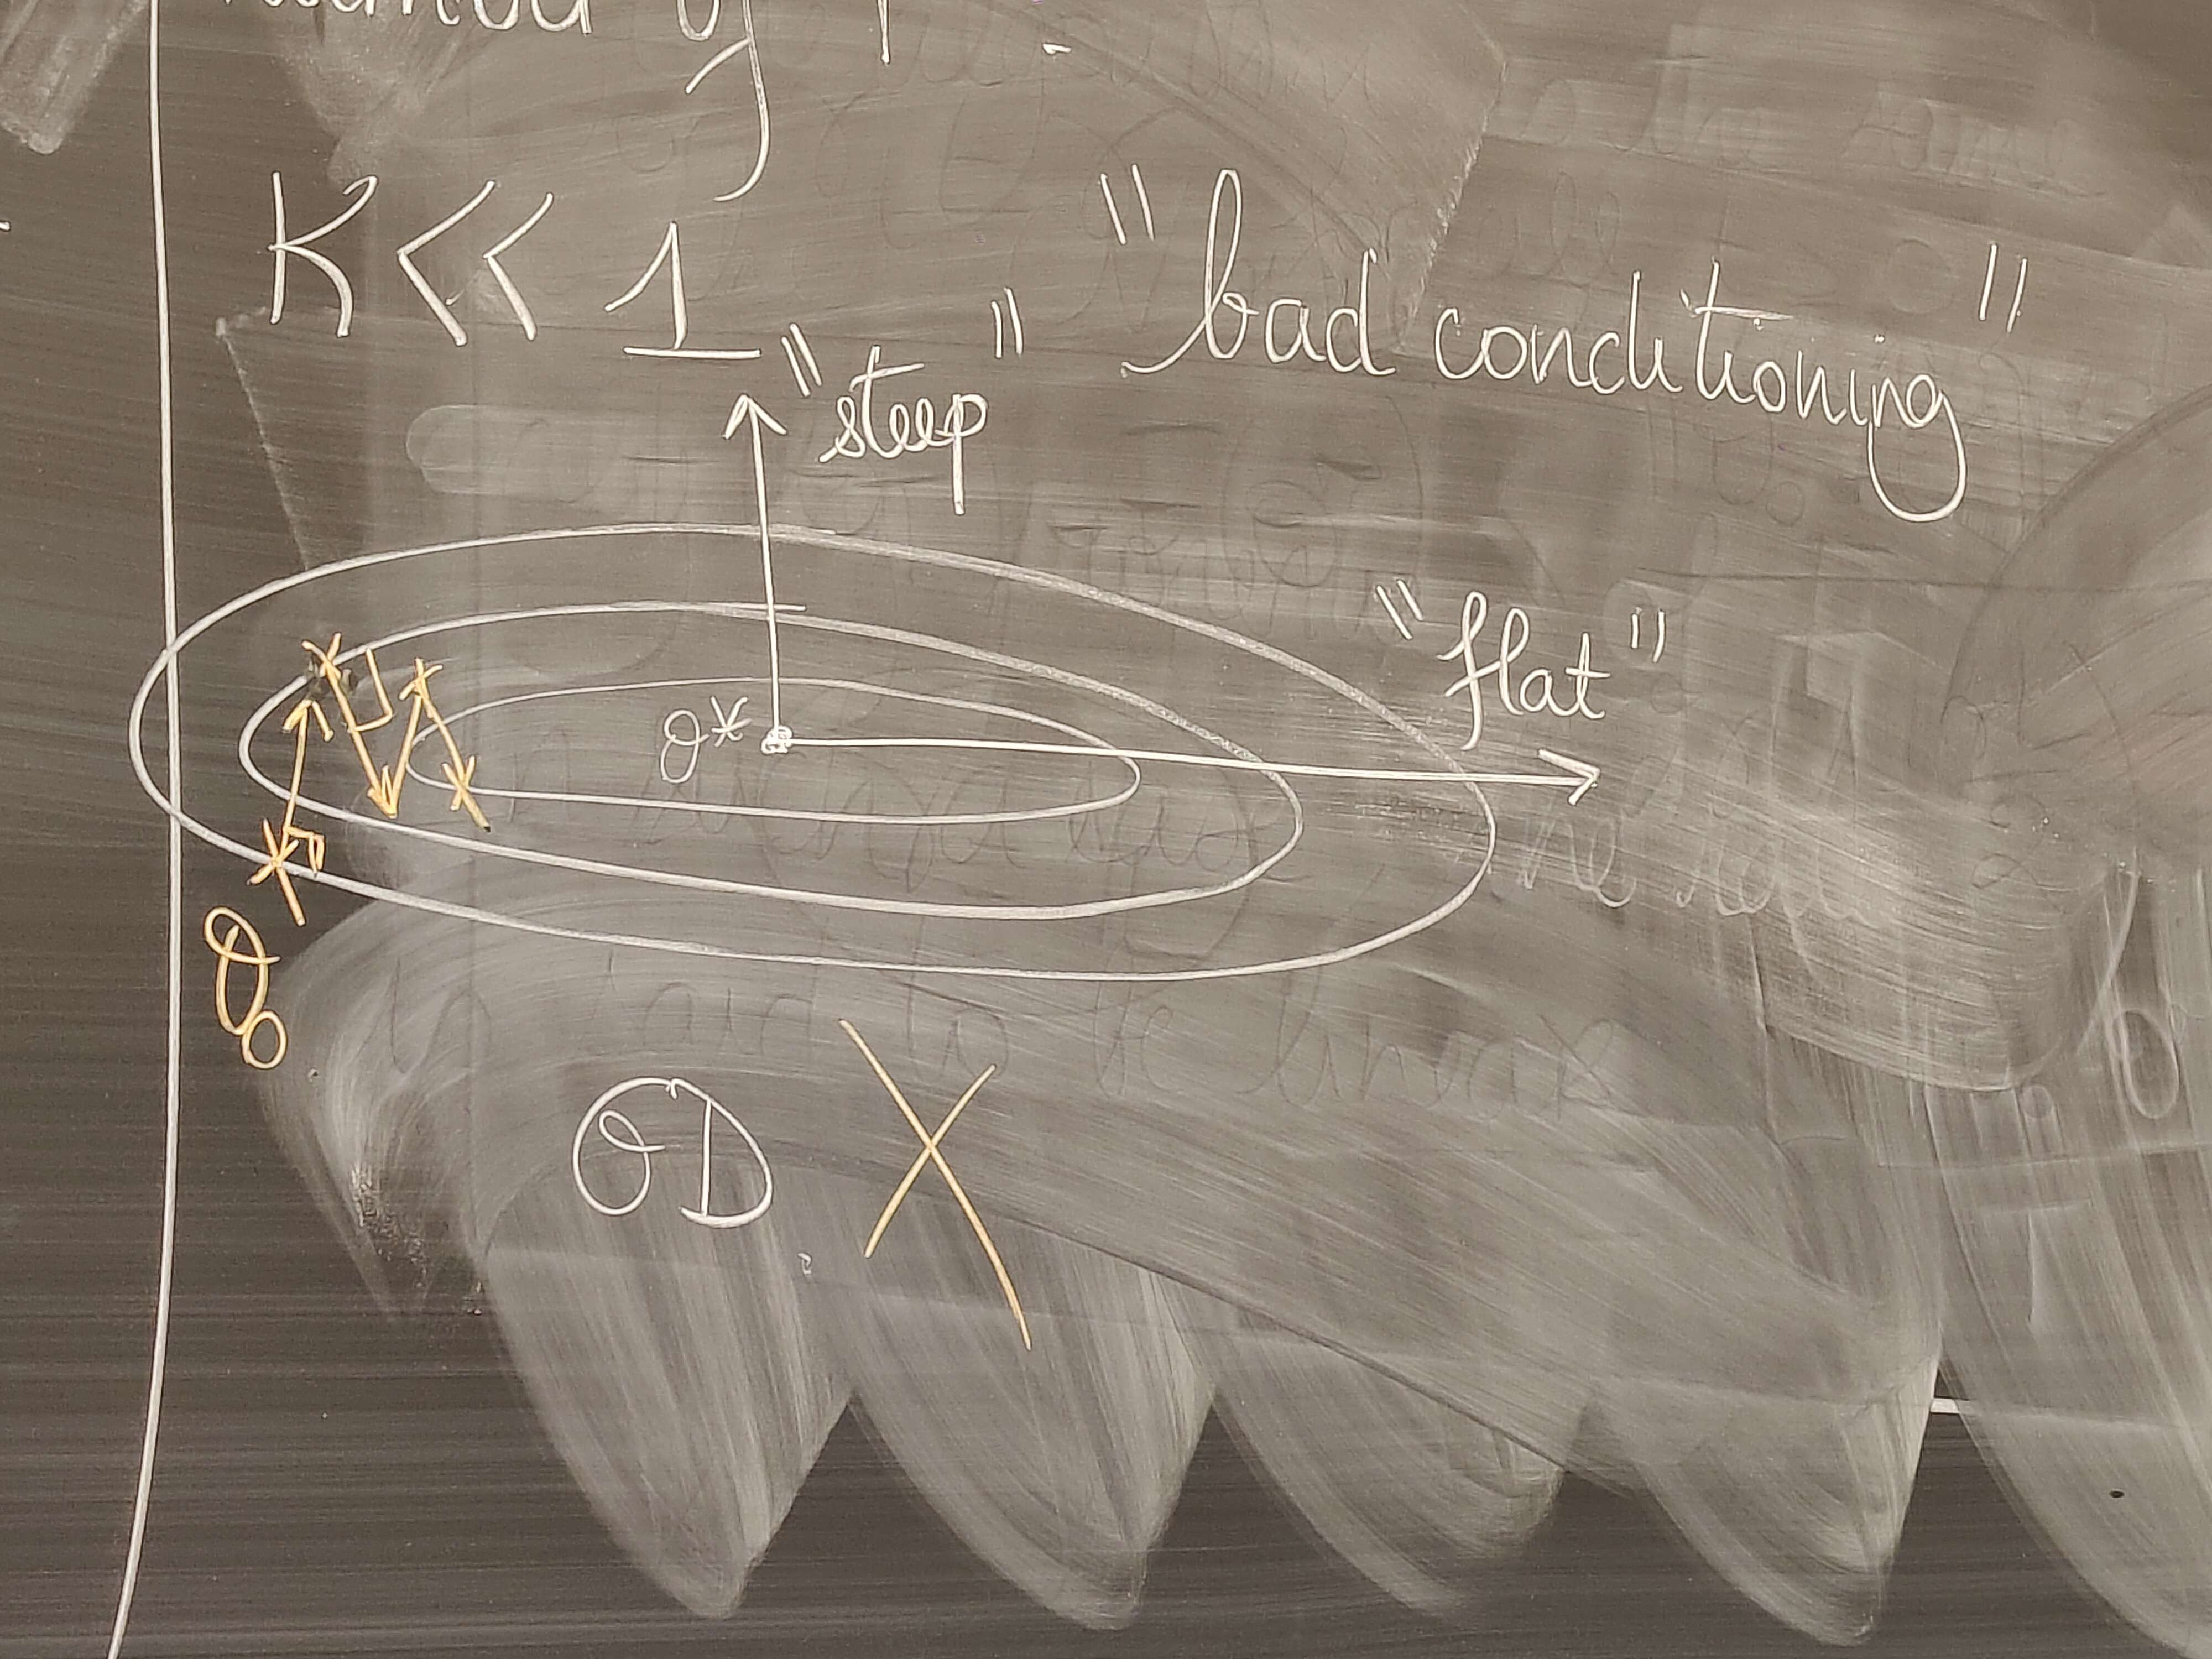
\includegraphics[width=.5\textwidth]{figs/bad_kappa.jpg}
        \caption{With $ \kappa \ll 1 $ "bad conditioning" }
    \end{figure}
    
    \begin{figure}[!htbp]
        \centering
        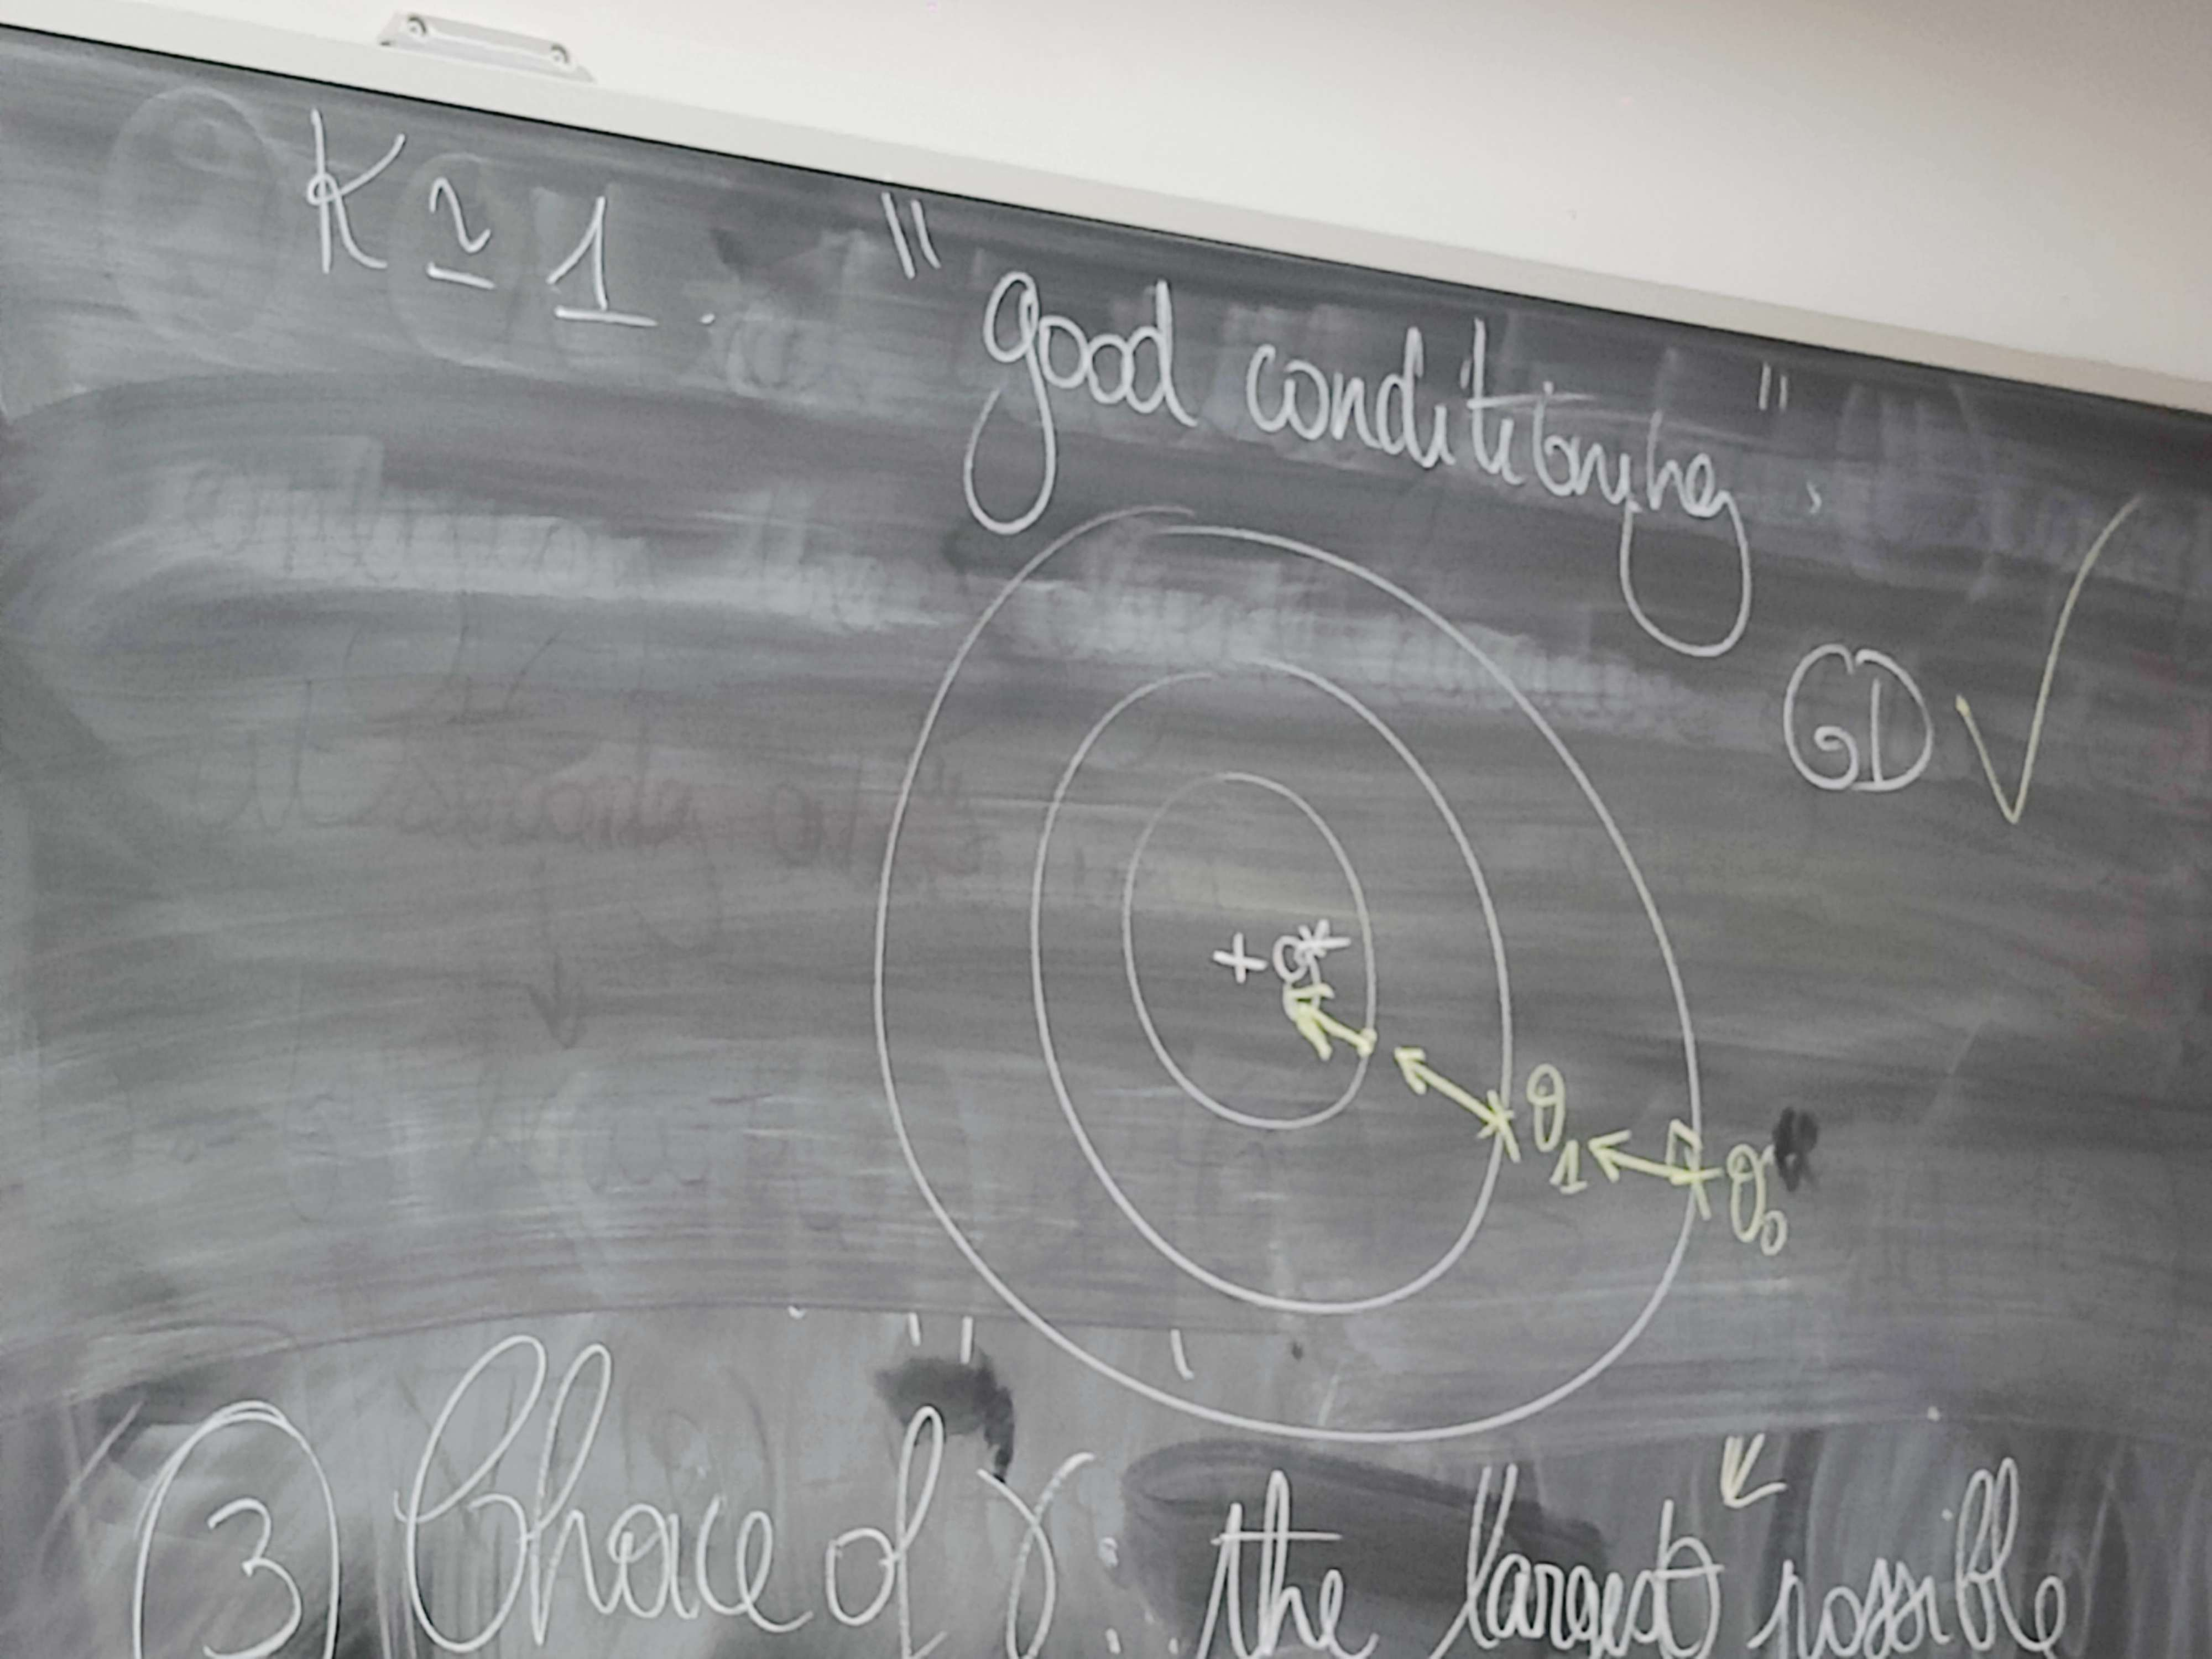
\includegraphics[width=.5\textwidth]{figs/good_kappa.jpg}
        \caption{With $ \kappa \approx 1 $ "good conditioning" }
    \end{figure}

    \begin{proof}[Proof:]
        \begin{align*}
            \left\| \theta _{t+1} - \theta ^\star  \right\| ^2 
                &= \left\| \theta _t - \gamma \nabla F(\theta _t) - \theta ^\star  \right\| ^2 \\
                &= \left\| \theta _t - \theta ^\star  \right\| ^2 - 2 \gamma \left\langle \nabla F (\theta _t), \theta _t - \theta ^\star  \right\rangle + \gamma ^2 \left\| \nabla F(\theta _t) \right\| ^2 \\
                &= \left\| \theta _t - \theta ^\star  \right\| ^2 + 2 \gamma \left\langle \nabla F (\theta _t), \theta ^\star - \theta _t \right\rangle + \gamma ^2 \left\| \nabla F(\theta _t) \right\| ^2 \\
        \end{align*}
        By $ \mu  $-strong convexity, we got 
        \begin{align*}
            &F(\theta ^\star ) \geq F(\theta _t) + \left\langle \nabla F(\theta _t) , \theta ^\star - \theta _t  \right\rangle + \frac{\mu }{2}\left\| \theta ^\star - \theta _t \right\| ^2 \\
            & \Rightarrow \left\langle \nabla F(\theta _t) , \theta ^\star - \theta _t \right\rangle \leq F(\theta ^\star ) - F(\theta _t) - \frac{\mu }{2}\left\| \theta ^\star -  \theta _t \right\| ^2
        \end{align*}
        
        Therefore $\left\| \theta_{t+1} - \theta^{\star }  \right\|^2 \leq \left\| \theta_t - \theta^{\star }\right\|^2 - 2 \gamma (F(\theta_t) - F(\theta ^{\star }) + \dfrac{\mu}{2} \left\| \theta ^{\star } - \theta_t \right\|^2 ) + \gamma ^2 \left\| \nabla F(\theta_t ) \right\|^2    $

        Beside, by L-smoothness, we get 
        \begin{align*}
            F(\theta _{t+1}) - F(\theta _t) 
                &= F(\theta _t - \gamma \nabla F(\theta _t)) - F(\theta _t) \\
                &= [F(\theta _t - \tau \nabla F(\theta _t))]^\gamma _{\tau = 0} \\
                &= -\int_{0}^{\gamma } \left\langle \nabla F(\theta _t), \nabla F(\theta _t - \tau \nabla F(\theta _t)) \right\rangle d \tau \\
                &= -\int_{0}^{\gamma } \left\langle \nabla F(\theta _t), \nabla F(\theta _t - \tau \nabla F(\theta _t)) \right\rangle + \left\| \nabla F(\theta _t) \right\|^2  - \left\| \nabla F(\theta _t) \right\|^2 d \tau \\
                &= - \gamma \left\| \nabla F(\theta _t) \right\| ^2 + \int_{0}^{\gamma } \left\langle \nabla F(\theta _t), \nabla F(\theta _t) - \nabla F(\theta _t - \tau \nabla F(\theta _t)) \right\rangle d \tau \\
                &\leq - \gamma \left\| \nabla F(\theta _t)  \right\| ^2 + \int_{0}^{\gamma }\tau L \left\| \nabla F(\theta _t) \right\| ^2 d \tau \quad \text{ (using CS + L-smooth)} \\
                &\leq - (\gamma - \frac{\gamma ^2 L}{2}) \left\| \nabla (F(\theta _t )) \right\| ^2 
        \end{align*}
        Combining the 2 previous inequalities, 
        \begin{align*}
            \left\| \theta_{t+1} - \theta ^{\star} \right\|^2 &\leq  \left\| \theta_{t} - \theta ^{\star} \right\|^2 (1 - \gamma \mu ) - 2 \gamma (F(\theta_t) - F^{\star }) + \frac{\gamma ^2 }{\gamma - \gamma^2 \frac{L}{2}} \\
            &\leq (1 - \gamma \mu ) \left\| \theta_t - \theta ^\star  \right\| ^2 - \gamma ( \frac{2 \gamma - \gamma ^2 \frac{L}{2} - \gamma }{\gamma - \gamma ^2 \frac{L}{2}}) ( F(\theta _t ) - F^\star )
        \end{align*}
        using that $ F(\theta ) \geq F(\theta ^\star ) \Rightarrow F(\theta _t) - F(\theta _{t+1}) \leq F(\theta _t) - F(\theta ^\star ) $  
        \begin{itemize}
            \item Numerator $ > 0 $  when $ 0 < \gamma \leq 1/L $ 
            \item Denominator $ > 0 $  when $ 0 < \gamma < 2/L $ 
        \end{itemize}
        Then by assuming $ \gamma \leq \frac{1}{L} $ just ignore the last term and conclude
    \end{proof}
\end{note}



\subsubsection{Subgradient method}
\begin{thm}[GD for non-smooth fonctions]
    Hypothese : $ F $ convex, has subgradients, $ \beta  $ -Lipschitz 
        \[
            \begin{cases}
                \left\| \nabla F(\theta ) \right\| ^2 &\leq \beta ^2\\
                \left\| \eta  \right\| ^2 &\leq \beta ^2, \quad \forall \eta \in \partial F(\theta)
            \end{cases} 
        .\]
    Then GD iterates with Polyak-Ruppert averaging enjoy the following error bound 
    
    \[
        \bar{\theta }_T = \frac{1}{T} \sum_{t=1}^{T} \theta _t
    .\]
    
    \begin{align*}
        F(\bar{\theta_T}) - F(\theta ^{\star}) 
            &\leq \frac{\left\| \theta_0 - \theta ^{\star } \right\|^2 }{2 \gamma T} +  \frac{\gamma \beta ^2}{2} \\
            &= \textcolor{orange}{\left\| \frac{\theta _0 - \theta^{\star }}{\sqrt[]{T}} \right\| \text{ for } \gamma = \gamma ^{\star}} 
        \text{ (when looking at below figures)}
    \end{align*}
    \[
        F(\bar{\theta_T}) - F(\theta ^{\star}) \leq \frac{\left\| \theta_0 - \theta ^{\star } \right\|^2 }{2 \gamma T} +  \frac{\gamma \beta ^2}{2}     
    .\]
\end{thm}
NB: now there is a trade-off on the choice of $ \gamma  $. Now we have two terms : 
\begin{itemize}
    \item $ \frac{\left\| \theta_0 - \theta ^{\star } \right\|^2 }{2 \gamma T}  $ in purple in Figure \ref*{fig:tradeoff}
    \item $ \frac{\gamma \beta ^2}{2}  $ in green  in Figure \ref*{fig:tradeoff}
\end{itemize}
\begin{figure}[!h]
    \centering
    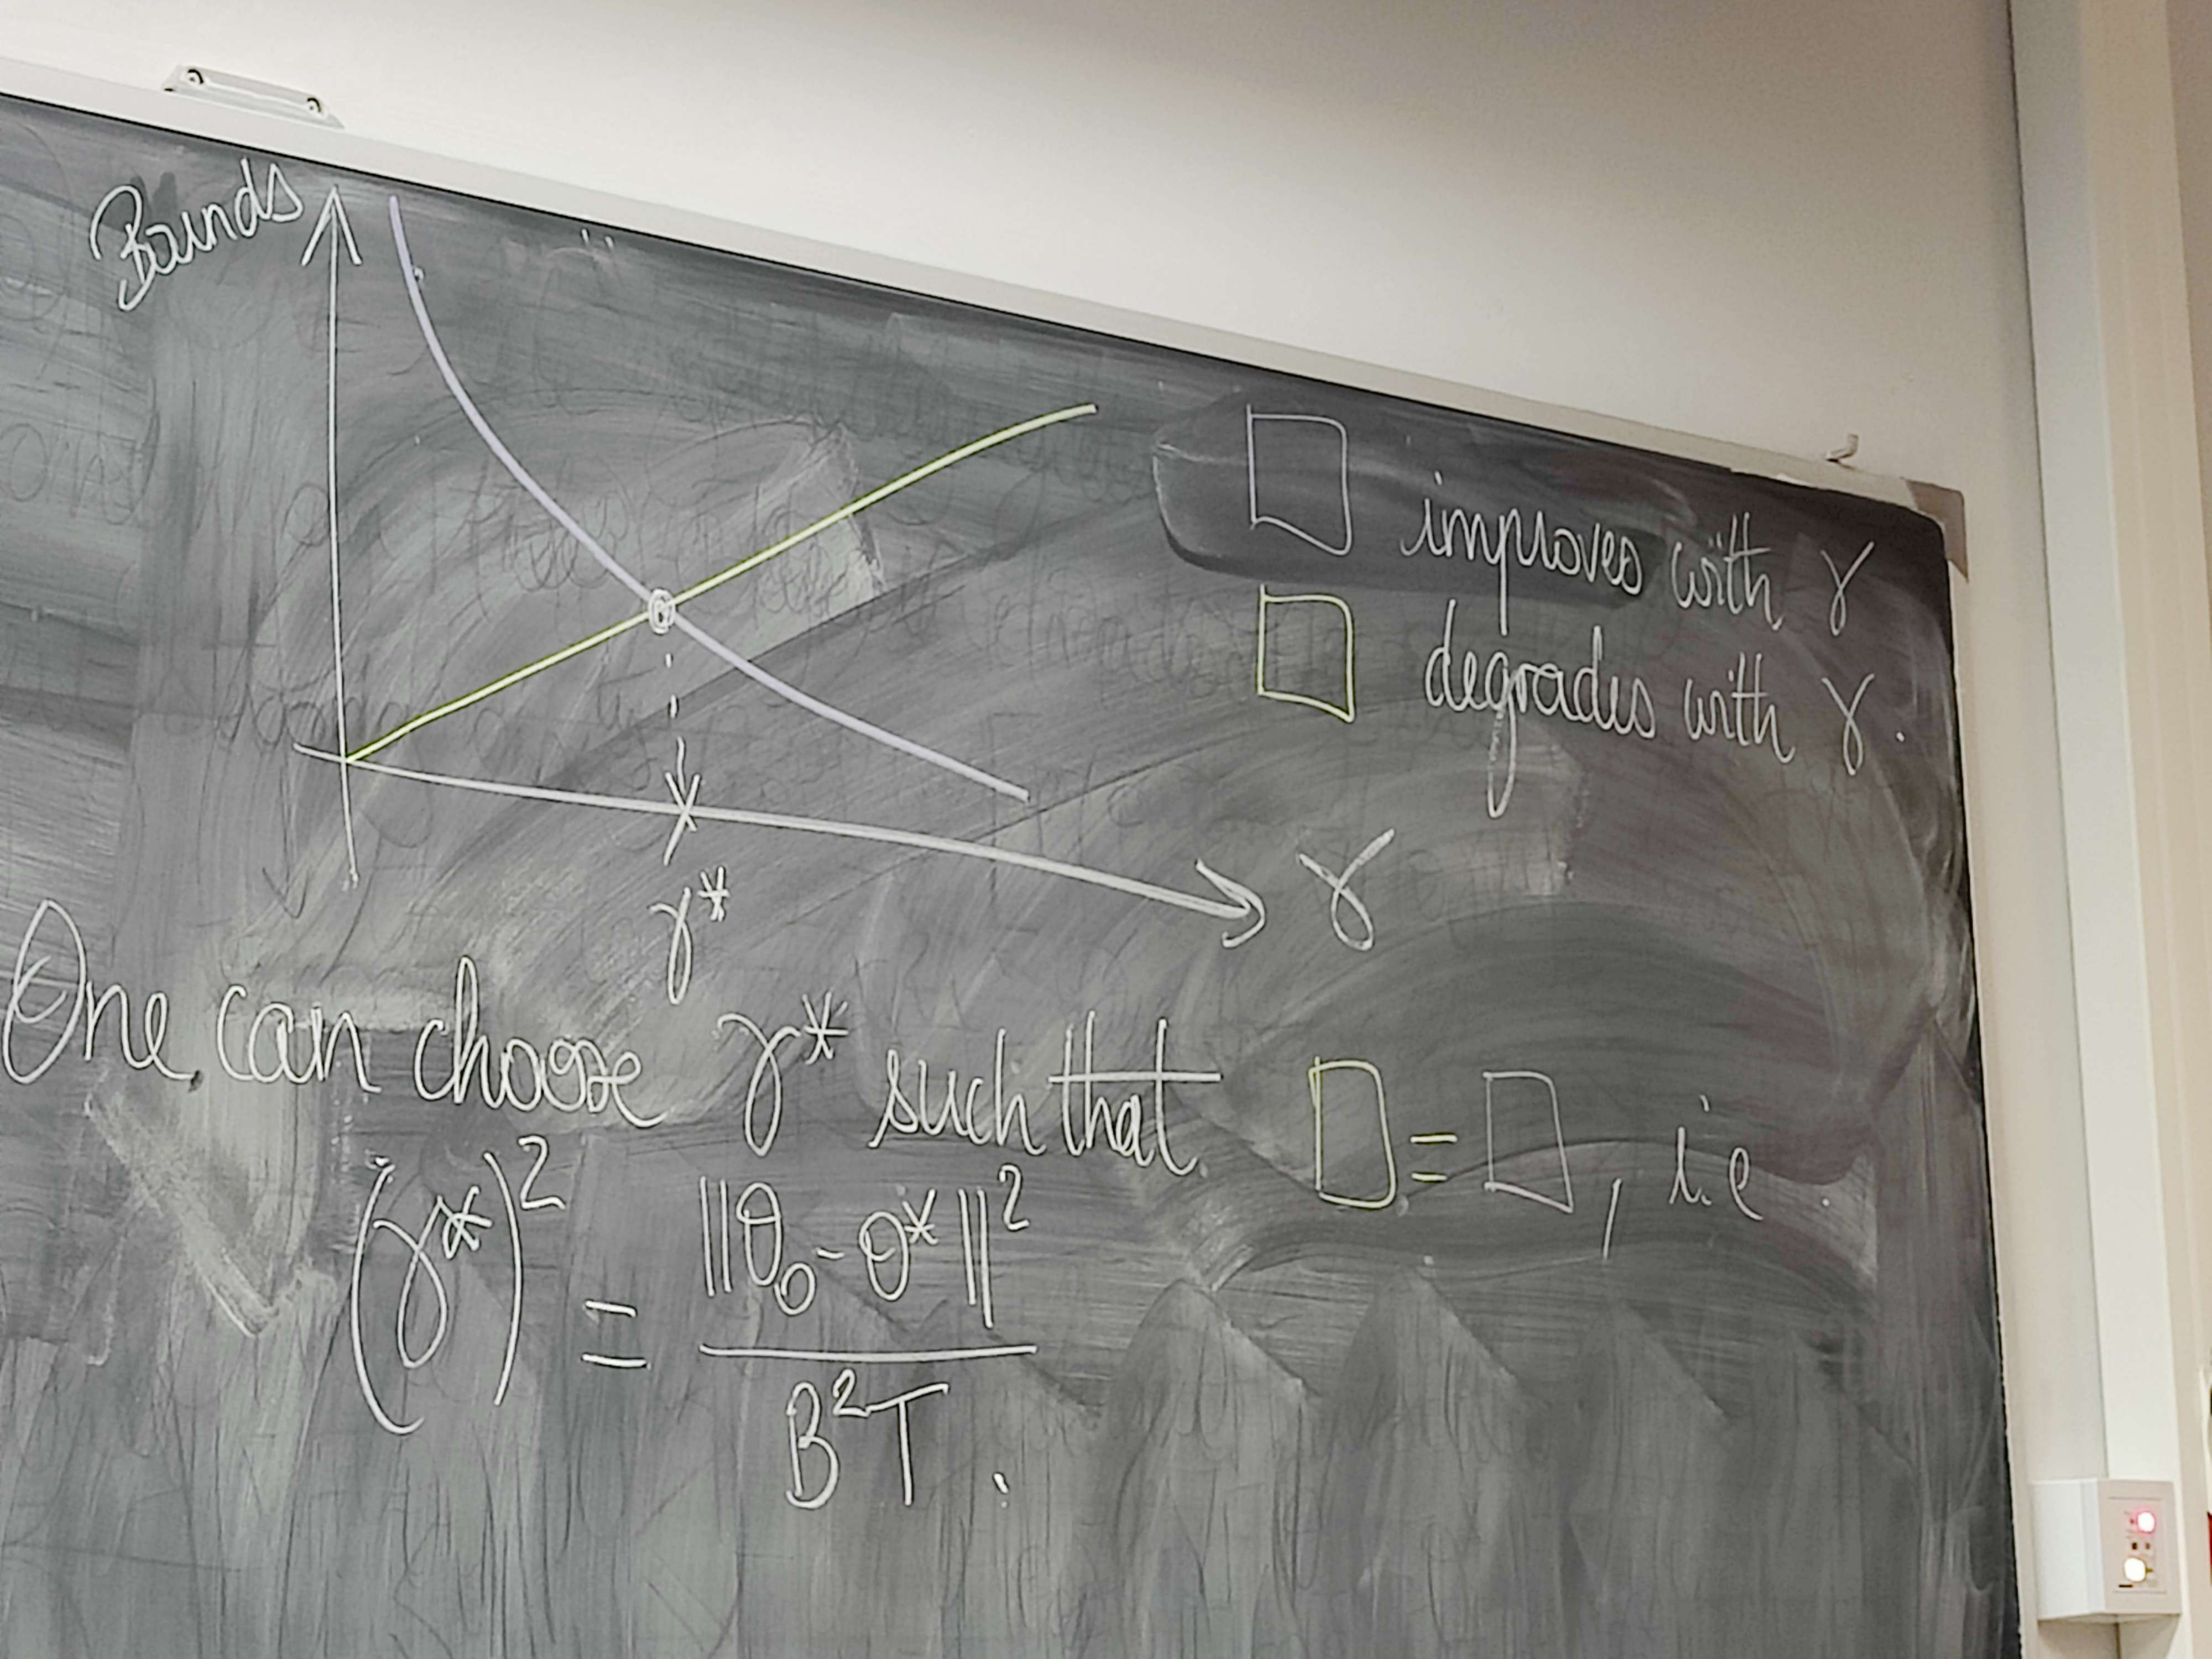
\includegraphics[width=.75\textwidth]{figs/gamma_compromise.jpg}
    \caption{ }
    \label{fig:tradeoff}
\end{figure}
One can choose $ \gamma ^\star  $ such that "purple" = "green" (Figre \ref*{fig:tradeoff}), i.e. 
\[
    (\gamma ^\star )^2 = \frac{\left\| \theta _0 - \theta ^\star  \right\| ^2}{\beta ^2 T}
.\]

\begin{itemize}
    \item Non-smoothness is paid through a $ O(\frac{1}{\sqrt[]{T}}) $ rate. 
    
    \item Guarantee for $ \bar{\theta} _T $ 
    
    \item CCL Big picture : BD-Based strategies 
    \begin{itemize}
        \item convex non-smooth $ O(1 / \sqrt[]{T}) $ 
        \item convex L-smooth $ O(1 / T) $ 
        \item $ mu $-strongly convex non-smooth $ O( ( 1 - \frac{\mu }{L})^T ) $ 
    \end{itemize}
\end{itemize}
$F(\frac{1}{T} \sum^T_{t=1} \theta_t) - F^{\star } \leq \frac{1}{T} \sum^T_{t=1} (F(\theta _t) - F^{\star })$ by convexity. \\
And $(F(\theta _t) - F^{\star })$ is on $\frac{1}{t}$ \\
So, $F(\frac{1}{T} \sum^T_{t=1} \theta_t) - F^{\star } \leq \frac{1}{T} \sum^T_{t=1} (F(\theta _t) - F^{\star }) \lesssim \mathcal{O}(\frac{\log_{T}}{T})$.

\begin{proof}[Proof:]
    \begin{align*}
        \left\| \theta _{t + 1} - \theta ^\star  \right\| ^2 
            &= \left\| \theta _t - \gamma _t g_t - \theta ^\star  \right\| ^2 \text{ with } g_t \in \partial F(\theta _t) \\
            &= \left\| \theta _t - \theta ^\star  \right\| ^2 - 2 \gamma _t \left\langle g_t , \theta _t - \theta ^\star \right\rangle + \gamma _t ^2 \left\| g_t \right\| _2 ^2 \\
            \text{by def of subgradient } &\leq \left\| \theta _t - \theta ^\star  \right\| ^2 - 2 \gamma _t (F(\theta _t) - F^\star ) + \gamma _t ^2 \left\| g_t \right\| _2 ^2 
    \end{align*}
    Recursively we obtain 
    \[
        \left\| \theta _{t+1} - \theta ^\star  \right\| ^2 \leq  \left\| \theta _1 - \theta ^\star  \right\| ^2 - 2 \sum_{s=1}^{t} \gamma _s (F(\theta _s) - F^\star ) + \sum_{s=1}^{t} \gamma _s ^2 \left\| g_s \right\| _2 ^2 
    .\]
    
    Combining this with $\sum_{s=1}^t \gamma _s (F(\theta _s) - F^{\star }) \geq \sum_{s=1}^t \gamma_s. \min_{1 \leq s \leq t} (F(\theta _s) - F^{\star })$ \\
    $\gamma$ cte + polyak- Ruppert \\
    $t \sum_{s=1}^t \frac{\gamma_s}{t}(F(\theta _s) - F^{\star }) \geq t \gamma (F(\bar{\theta _t}) - F^{\star })$ 


    Finally, 
    \begin{align*}
        \min _{1 \leq s \leq t} F (\theta _s) - F^\star 
        &\leq \frac{\left\| \theta _1 - \theta ^\star  \right\|_2 ^2 + \sum_{s=1}^{t} \gamma _s \left\| g_s \right\|_2 ^2  }{2 \sum_{s=1}^{t} \gamma _s} \\
        &\leq \frac{\left\| \theta _1 - \theta ^\star  \right\|_2 ^2 + \beta ^2 \sum_{s=1}^{t} \gamma _s  }{2 \sum_{s=1}^{t} \gamma _s} \\
        F(\bar{\theta}_t) - F^\star &\leq \frac{\left\| \theta _1 - \theta ^\star  \right\| ^2 + t \gamma ^2 \beta ^2}{2t \gamma}
    \end{align*}
\end{proof}

\begin{note}[Implicit gradient method]
    Subgradient method = generalization of GD in the non-smooth case but $ O $ is typically slow ($ \frac{1}{\sqrt[]{T}} $ ). 

    The essential reason is that there are plenty of subgradients that are large near and event at the solution.

    $ g \in \partial F(\theta ) $ if $ \forall \theta ^\prime, F(\theta ^\prime ) \geq F(\theta ) +  \left\langle g, \theta ^\prime - \theta  \right\rangle $ 
    \[
        \partial ? (\theta ) = \begin{cases}
            \{ +1 \}  &\text{ if } \theta > 0\\
            \{ -1 \}  &\text{ if } \theta < 0\\
            [-1 , 1]  &\text{ if } \theta = 0\\
        \end{cases} 
    .\]
    
    \begin{figure}[!h]
        \centering
        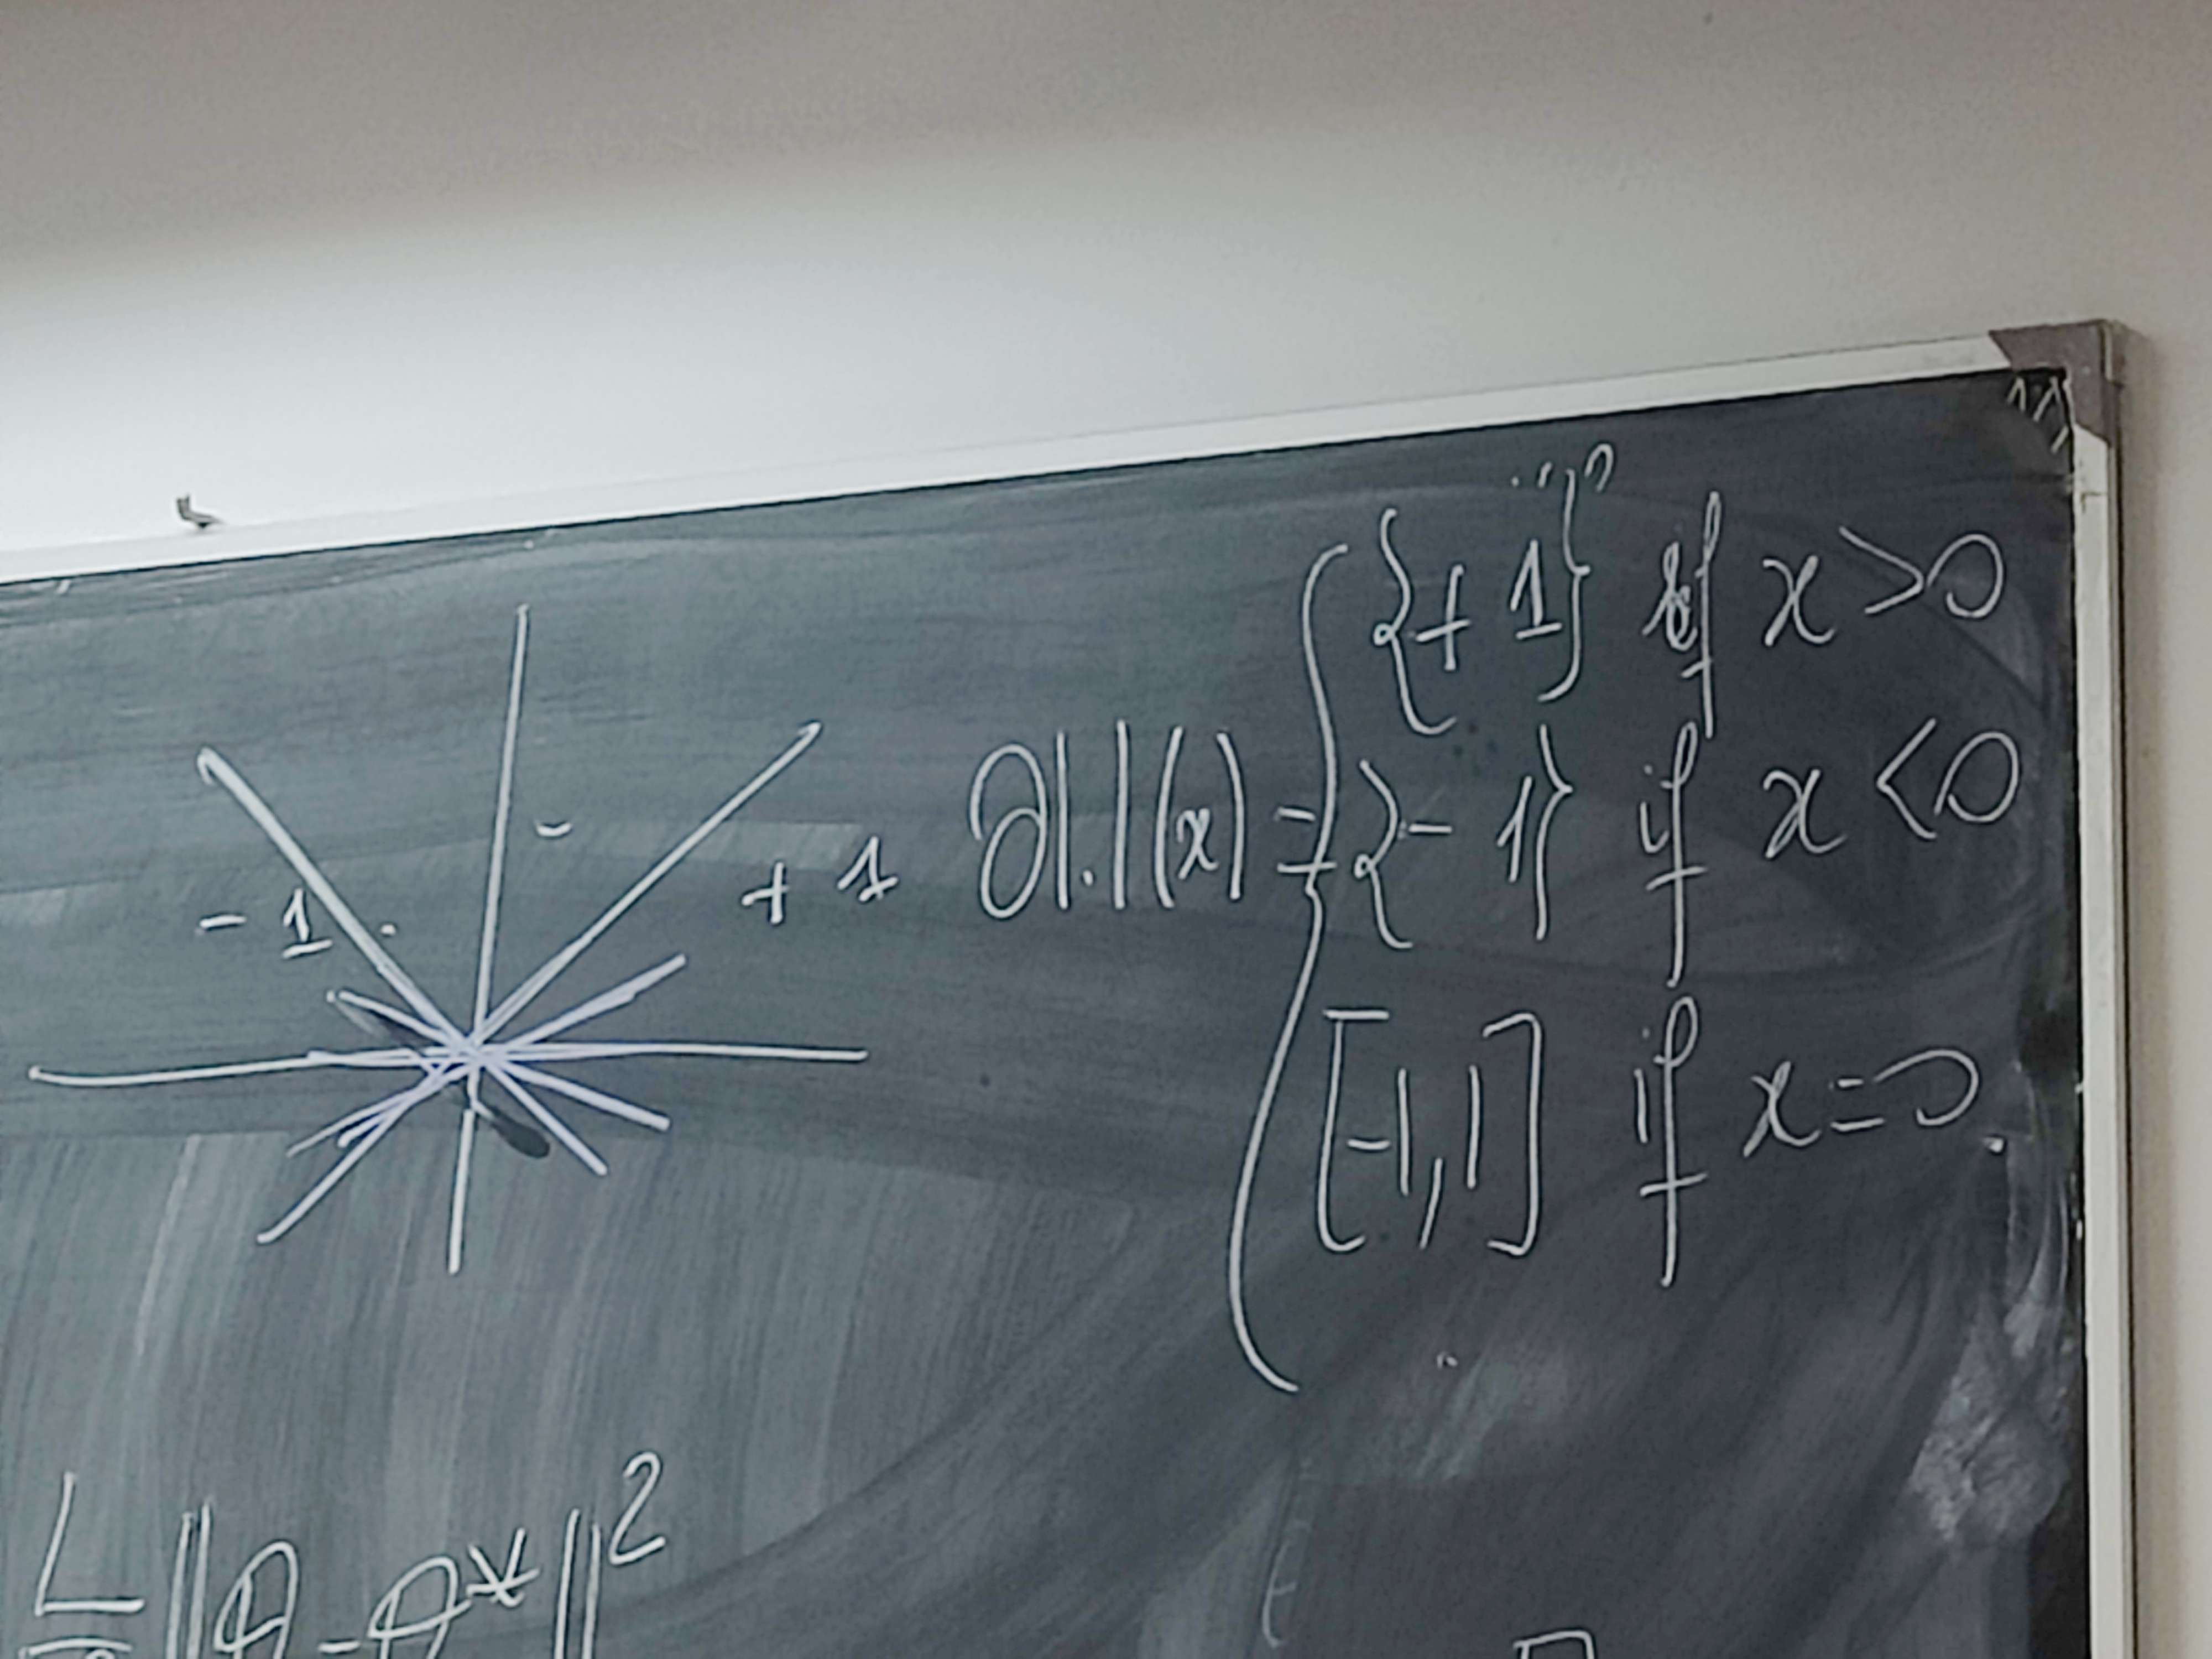
\includegraphics[width=.65\textwidth]{figs/subgradients.jpg}
        \caption{sub gradiens}
        \label{truc}
    \end{figure}

    Another way to deal with this is to add a smooth regularized term. In particular, if $\theta ^{\star }$ is minimizer of F then it minimizes as well
    \[ \theta  \mapsto F(\theta) + \gamma \left\| \theta - \theta ^{\star } \right\| \text{ for } \gamma > 0  \]

    Now the regulatized fonction is strongly convex and the only subgradient at the solution is the zero vector : \begin{itemize}
        \item \textbf{Good} : It addresses the main drawback of subgrad methods
        \item \textbf{Bad} : We have to know $ \theta ^\star  $ 
    \end{itemize}

    One can implement an iterative version of it, this is the proximal algo : 
    \[ 
        \theta _{t+1} = \arg \min_{\theta} F(\theta) + \frac{1}{2 \gamma _t} \left\| \theta - \theta_t  \right\|^2 
    \]
    When $ F $ is convex, $ F + \frac{1}{2 \gamma _t} \left\| \circ  - \theta _t \right\| ^2 $ is strictly convex so the mapping is well defined. This gives the proximal operator / Moreau envelope. 
    
    \[
        prox _{\gamma _t F} (\theta ) = \arg \min_{\tilde{\theta}} F(\tilde{\theta }) + \frac{1}{2 \gamma _t} \left\| \theta - \tilde{\theta}  \right\|^2 
    .\]

    The proximal operator can be interpreted as a variation of gradient methods 
    
    \[
        \begin{cases}
            \frac{d \theta }{dt}(t) = - \nabla F(\theta ) \\
            \theta (0) = \theta _0 \in \mathbb{R}^d
        \end{cases}
    .\]
    The equilibrium points of this system are the $\theta $'s such that $\nabla F(\theta )= 0$, i.e the minimizers of $ F $  when $ F $  is convex
    
    GD = 1st order numerical method for tracing the path from $ \theta _0 $ to $ \theta ^\star  $ 
    \[
        \frac{\theta (t + h) - \theta (t)}{h} \approx - \nabla F(\theta (t))
    .\]
    
    GD $\equiv$ Forward Euler discretization. \\
    But we could use Backward instead 
        
    \[
        \frac{\theta (t) - \theta (t -h)}{h} \approx - \nabla F(\theta (t))
    .\]
    And now the iterates obey :
    \[
        \theta_{t+1} = \theta _t - h \nabla F(\theta_{t+1}) \qquad \text{"Implicit"}
    .\]
    Their construction is not straight forward anymore. But this is what the prox operator actually computes 
    \begin{align*}
        \theta _{t+1} = \arg \min F(\theta _t) + \frac{1}{\gamma _t } \left\| \theta -\theta _t \right\| ^2 \\
        \Leftrightarrow 0 = \nabla F(\theta _{t + 1}) + \frac{1 }{\gamma _t} (\theta _{t+1} - \theta _t)
    \end{align*}
\end{note}


\begin{note}[Newton's method]
    Given $ \theta _{t-1} $, the Newtons's method minimizes the 2nd ordre Taylor expansion arount $ \theta _{t-1} $ 
    \[
        \theta \mapsto F(\theta_{t-1}) + \left\langle \nabla F(\theta _{t-1}, \theta  - \theta _{t-1}) \right\rangle + \frac{1}{2} (\theta  - \theta _{t-1} )^T Hess_F(\theta _{t-1}) (\theta - \theta _{t-1})
    .\]
    the gradient of this quadratic form is 
    \[
        \nabla F(\theta _{t-1}) + H_F(\theta _{t-1})^{-1} \nabla F(\theta _{t-1})
    .\]
    Exercise : Check that $- H_F(\theta_{t-1})^{-1} \nabla F(\theta_{t-1})$ is indeed a descent direction of F at $\theta_{t-1}$.
    
    Newton's method are methods of order 2 : using the gradient (order 1) and the Hessian (order 2). Running-time complexity is $ O(d^3) $ in general to solve the linear system. 

    It leads to local quadratic CV : 
    \[
        (C \left\| \theta_t - \theta ^{\star}\right\| ) \leq (C \left\| \theta_t - \theta ^{\star}\right\| )^2
    .\]
    For global convergence guarantees, see  \textit{Boyd \& Vandenberghe (2004)} in particular using the self-concordance relating 3rd and 2nd order derivatives. 
\end{note}

\section{Inertial methods}

\subsection{Préliminaries}
So far we have \begin{itemize}
    \item convex, L-smooth : $ O(1/k) $ 
    \item strongly convex, L-smooth : $ O((1 - \frac{\mu }{L}) ^k ) $ 
\end{itemize}

Can we do better with a \textbf{gradient-like} algo ? 

\begin{defn}[]
    A gradient-like algo is an algo such taht 
    \[
        \theta _{t+1} \in span \{\theta _0, \dots, \theta _t, \nabla F(\theta _0), \dots, \nabla F(\theta _t)\}
    .\]
\end{defn}

\begin{thm}[Nemirovski-Rudin 1983]
    $\forall \theta_0 \in \mathbb{R}^d, \forall 0 \leq t \leq \frac{d-1}{2}$ \\
    $ \exists F $  convex, L-smooth such that for every gradient-like algon we have 
    \[
        F(\theta _t) - \inf F \geq \frac{3L \left\| \theta ^0 - \theta ^\infty  \right\| }{32 \mathbf{(t + 1)^2}}
    .\]
\end{thm}

\begin{thm}[Nesterov 2003]
    $ \forall \theta _0 \in \mathbb{R}^d, \mu > 0, L > 0, \exists F $ $ mu $-strongly convex and L-smooth such that for every gradient-like algo \begin{enumerate}
        \item $ F(\theta _t) - \inf F \geq  \frac{\mu }{2} ( \frac{1 - \sqrt[]{\kappa }}{1 + \sqrt[]{\kappa }} )^{2t} \left\| \theta _0 - \theta ^\star  \right\|  $ 
        \item $\left\| \theta _t - \theta ^{\star } \right\| \geq (\frac{1 - \sqrt[]{\kappa }}{1 + \sqrt[]{\kappa }})^t \left\|  \right\| \theta _0 - \theta ^{\star } \quad $ with $\kappa = \frac{\mu }{L}$ 
    \end{enumerate}
\end{thm}

Can we design first-order strategies that achieve convergence rates matching these lower bounds ? 

\subsection{Heavy ball dynamics}

\[
    \ddot{\theta }(t) = - \alpha (t) \dot{\theta } - \nabla F(\theta (t)), (\alpha (t) > 0 )
.\]
We add a function term to the gradient flow. 

We can have a look at the quantity 
\[
    \epsilon (t) = F(\theta (t)) - \inf F + \frac{1}{2} \left\| \dot{\theta }(t) \right\| ^2 = E_{pot} + E_{cin}
.\]

We can show that $ \epsilon (t) $ is decreasing (this is a Lyapunov energy) 
\begin{align*}
    \dot{\epsilon }(t) \\
        &= \left\langle \nabla F(\theta (t)) , \dot{\theta }(t) \right\rangle + \left\langle \ddot{\theta }(t) , \dot{\theta }(t) \right\rangle \\
        &= \left\langle \ddot{\theta }(t) + \nabla F(\theta (t)), \dot{\theta }(t) \right\rangle \\
        &= - \alpha (t) \left\| \dot{\theta }(t) \right\| ^2 \mathbf{()\leq 0)}
\end{align*}

\begin{note}
    $ \alpha (t) \equiv 0 $  gives a conservative dynamics with aliittle hope of CV.

    \begin{align*}
        F(\theta ) &= \frac{1}{2}\theta ^2, \alpha = 0 \\
        \ddot{\theta }(t) &= - \theta (t) \Leftrightarrow \theta (t) = c_1 \sin (t) + c_2 \cos (t)
    \end{align*}
    Why it can help? Gabriel Goh "Why momentum really works".
    \[
        \ddot{\theta }(t) = - \alpha (t) \dot{\theta }(t) - \nabla F(\theta (t))
    .\]
    
    \paragraph*{Discretization }
    \begin{align*}
        \theta (t_k) & \approx \theta _k \\
        \dot{\theta } (t_k) & \approx \frac{\theta _k - \theta _{k-1}}{h} \\
        \ddot{\theta } (t_k) & \approx \frac{\dot{\theta }(t_{k+1}) - \dot{\theta }(t_k)}{h} \\
        \frac{\theta _{k+1} - 2 \theta _{k} + \theta _{k+1}}{h^2} + \alpha (t_k) \frac{\theta _{k}- \theta _{k-1} }{h} &+ \nabla F(\theta _{k}) = 0
    \end{align*}
    
    Define $\gamma = h^2$  $\alpha_k = \frac{\alpha (t_k)}{\sqrt[]{\gamma }}$ we get :
    \[
        \theta _{k+1} = \theta _{k} - \gamma \nabla F(\theta _{k}) + (1 - \alpha_k )(\theta _{k} - \theta _{k-1})
    .\]
    where $\gamma \nabla F(\theta _{k})$ is the gradient step and \\
    $ (1 - \alpha_k )(\theta _{k} - \theta _{k-1})$ is the inertia : memory of the last iterates. [polyak 64]


    \paragraph*{HEAVYBALL}[Polyak, 64]
    \begin{align*}
        \beta _k &= \theta _k + (1 - \alpha _k) (\theta _k - \theta _{k-1}) \\
        \theta _{k+1} &= \beta _k - \gamma \nabla F(\theta _k)
    \end{align*}

    \paragraph*{NESTEROV ALGO}[83]
    \begin{align*}
        \beta _k &= \theta _k + (1 - \alpha _k) (\theta _k - \theta _{k-1}) \\
        \theta _{k+1} &= \beta _k - \gamma \nabla F(\beta _k)
    \end{align*}

    They look the same, the only difference is where the gradient is evaluated. Both algo come with 2 choices for the friction $ \alpha _k $ \begin{itemize}
        \item constant friction $ \alpha _k \equiv \alpha \sqrt[]{\gamma } $ (for good functions)
        \item vanishing friction  $ \alpha _k \equiv \frac{\alpha}{k}  $ (for bad functions)
    \end{itemize}
\end{note}

\paragraph*{HEAVY BALL}
\begin{thm}[polyak 64, écrit vite fait parce que c'est la fin du cours]
    F quadratic -smooth, m$\mu$- strongly cvx, $\kappa = \frac{\mu }{L}$ with,

    \[
        \begin{cases}
            \gamma = \frac{4}{L(1+K)^2} \\
             \alpha _k = \frac{2 \sqrt[]{\mu } \gamma }{1 + \sqrt[]{\kappa }}
        \end{cases} 
    .\]
    CV rate $\mathcal{O}((\frac{1 - \kappa }{1 + \kappa })^t )$

    Cool : We have Optimal rate and constant friction is enough \\
    But : HB can fail on general strongly convex fonction and need to know $ \mu  $  (and $ L $ )
\end{thm}

\paragraph*{NESTEROV}
\begin{thm}[]
    F L-smooth, $\mu$-strongly cvx
    Choose $ \gamma  = 1/L, \alpha = \frac{\sqrt[]{L} - \sqrt[]{\mu }}{ \sqrt[]{L} + \sqrt[]{\mu }} $ to get $ (1 - \sqrt[]{\frac{\mu }{L}}) $ -linear CV (convergence)

    Cool : Better GD \\
    Questionnable : Not optimal
\end{thm}

\begin{thm}[Nesterov 83, Chambolle-Dossal 2015]
    F convex, L-smooth
    $ \gamma \leq 1/L, \alpha _k = \alpha / k $ with $ \alpha \geq 3 $ 
    \[
        F(\theta _k) - F^\star \leq O(\frac{1}{k^2})
    .\]
    
    Cool : Optimal
\end{thm}

We can take other choices for decreasing $(\alpha _k)_k$, the historical choice is


\[
    \text(Friction : )(1 - \alpha _k) = \frac{t_k - 1 }{t_{k+1}} \text{ with } \begin{cases}
        t_1 = 1 \\
        t_{k+1} = \frac{1 + \sqrt[]{1 + 4 t _k ^2}}{2} \\
    \end{cases} 
.\]
CCL : Essayer les deux méthodes : speed upped or not 

\begin{figure}[htbp]
    \centering
    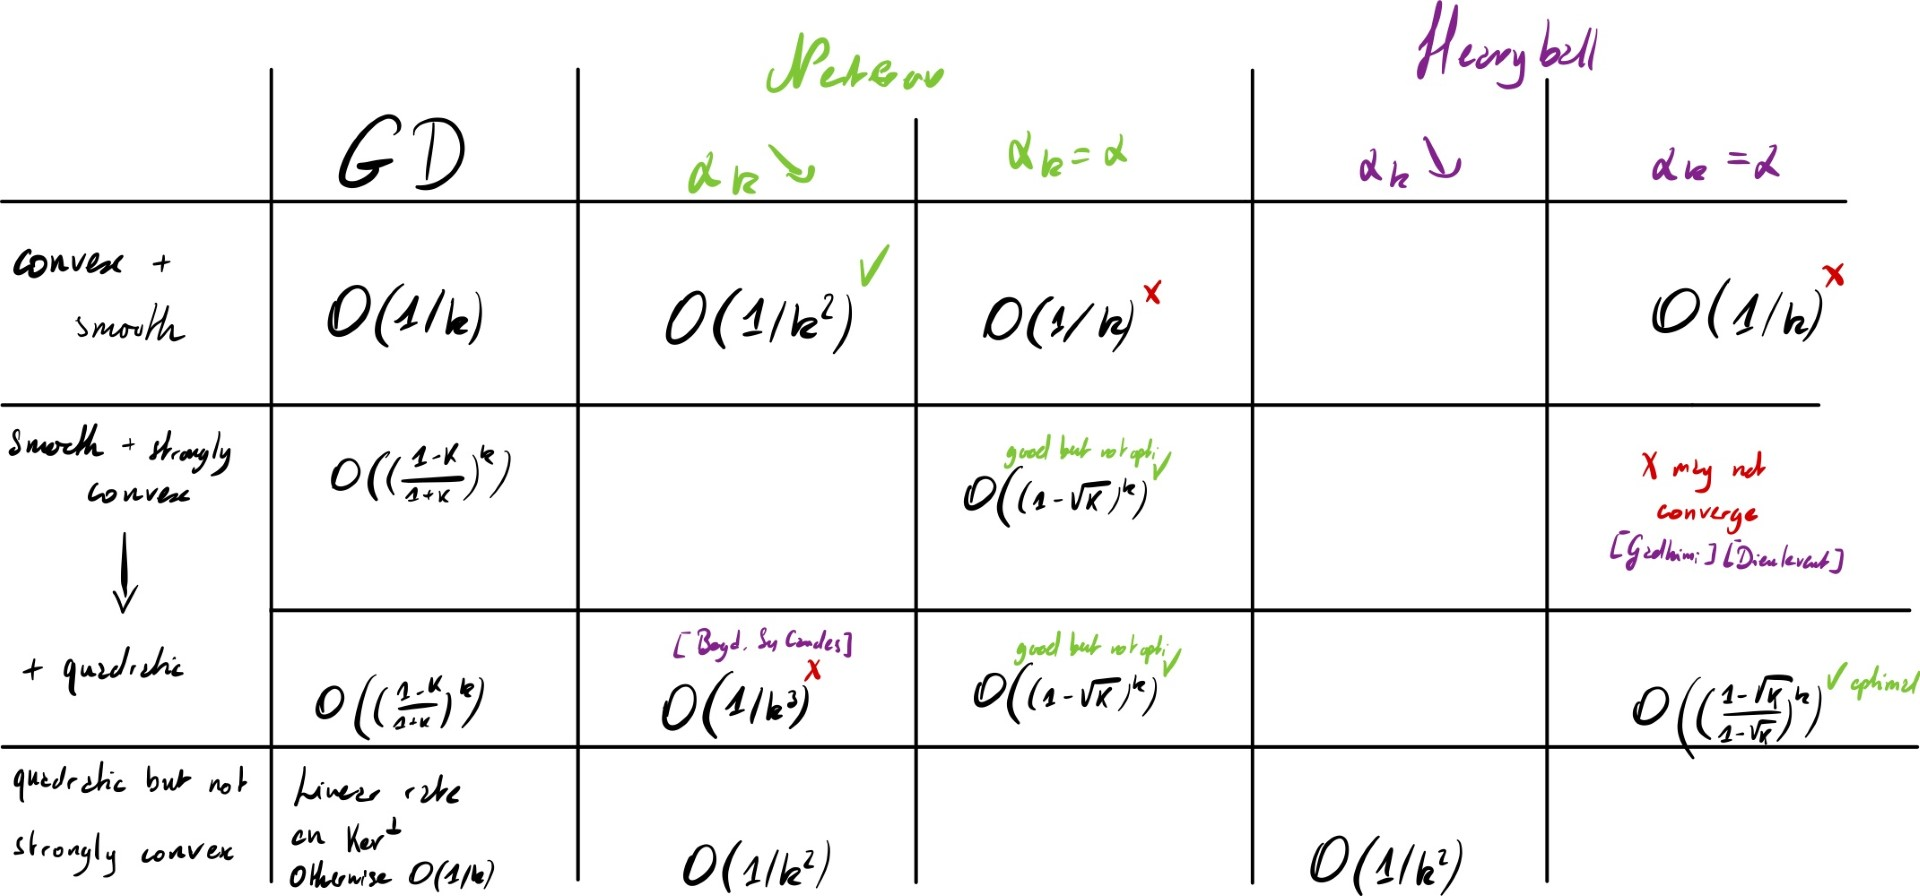
\includegraphics[width=.95\textwidth]{figs/table_conv_speed.jpg}
    \caption{Tableau de la vitesse de convergence des algos}
\end{figure}

CCL : vanishing friction helps on the worst fcts

\chapter{Stochastic Gradient Algorithms (SGD)}

\[
    \min _{\theta \in \mathbb{R}^d} F(\theta )
.\]

At any step, assume that we have access to a "random" direction / gradient : $ g_t : \mathbb{R}^d \to \mathbb{R}^d $ 


$ \forall t \geq 0 $, $ \theta_{t+1} = \theta_{t} - \gamma_t g_{t+1}(\theta_{t}) $ and $\gamma_t =$ (learning rate) / (step size)

Think of $ g_t $ as a noisy estimate of the "true" gradient, we would like to use instead 

\begin{figure}[htbp]
    \centering
    
    \caption{Noisy gradient descent}
\end{figure}

\textbf{Hypothesis}: [Unbiased estimates of the gradient]
\[
    \mathbb{E}[g_t(\theta _{t-1}) | \theta _{t-1}] = \nabla F(\theta _{t-1})
.\]

$\theta_{t-1}$ encapsulates all the randomness due to> the past iterations, so we only require "fresh" randomness at time $t$. \\

\section{SDG in machine learning}

There are 2 ways to use SGB in supervised learning 

\subsection{Empirical risk minimization}
If $F(\theta) = \frac{1}{n} \sum^n_{i=1}l(Y_i, f_\theta(X_i))$
then at iteration $ t $, we can choose uniformly at random $ i(t) \approx \mathcal{U} ( [1, n ]) $ 
and define $g_t$ as the gradient of $l_{i(t)} : \theta \mapsto l(Y_{i(t)}, f_{\theta}(X_{i(t)}))$
A full GD would use $ \nabla F(\theta ) = \frac{1}{n} \sum_{i=1}^{n} \nabla l_i (\theta ), g_t := \nabla l_{i(t)} (\theta ) $  for $ l_i (\theta ) = l(Y_i, f_\theta (X_i)) $, i.e. the $ n $ gradients of the terms composing the sum. SGD relies on a "moisy" estimate of $ \nabla F(\theta ) $ by selecting at random only one term $ \nabla l_{i(t)} $ 

Conditionnally to the training data, we aim at minimizing a deterministic fonctions using a stochastic algo to help on complexity issues. Indeed, the randomness comes from the random indeces $(i_(t))_t$. \\
There exist minibatch versions where at each iteration the gradient is estimated over a random subset of indices \\
\begin{itemize}
    \item reducing the variance of the estimated gradient
    \item increasing the running time
\end{itemize}
The theoritical analysis focuses on the CV to the ERM $\theta^{\star}$ :
\begin{align*}
    I &\sim \mathcal{U}([1; n]) \\
    \mathbb{E}[g_t(\theta) | \theta ] &= \mathbb{E}[ \nabla l_I (\theta ) | \theta ] = \sum_{i=1}^{n}\mathbb{P}(I = i) \nabla l_i (\theta ) \\
    &= \frac{1}{n} \sum_{i=1}^{n} \nabla l_i (\theta ) = \nabla F(\theta )
\end{align*}

We can select several times the same $\nabla l_i$ even within $n$ iterations sampling without replacement can be possible but its analysis is more involved (need to handle the bias) see Nagaraj et al 2019

\subsection{Expected risk minimization}

\[
    F(\theta ) = \mathbb{E}[l(Y, f_\theta (X))]
.\]
expected (non-observable) risk, then at each iteration $ t $, we can take $ (X_t, Y_t) $ and define $ g_t $ as the gradient of $ \theta \mapsto l(Y_t, f_\theta (X_t)) $ 
By swapping the order of expectation and differentiation, we can get unbiased estimators

\[
    \mathbb{E}_{(X_t,Y_t)}[\nabla_\theta l(Y_t, f_{\theta}(X_t)) ] = \nabla_{\theta} \mathbb{E}[l(Y_t, f_{\theta}(X_t))]_t
.\]

Sanity-check for linear regression : 
\[
    F(\theta ) = \mathbb{E} [ (Y - \left\langle X, \theta  \right\rangle )^2 ] = \mathbb{E}[ f(\theta )]
.\]
\[
    \nabla f(\theta ) = 2 ( \left\langle X, \theta  \right\rangle ) X
.\]
\[
    \left\| \nabla f(\theta ) \right\|  \leq 2 \left| \left\langle X, \theta  \right\rangle  - Y \right|  \left\| X \right\| 
.\]


 If $\forall \theta $, $\mathbb{E}[\left| \left\langle X, \theta \right\rangle  \right| \left\| X \right\| ] < + \infty $, the $\nabla _{\theta } F(\theta) = \nabla_{\theta} \mathbb{E}[(Y - \left\langle X, \theta \right\rangle )^2] = \mathbb{E}[\nabla _{\theta}f(\theta)]$

Note that to preserve the unbiasedness, only a \textbf{signle pass} is allowed. \\
Here, we directly minimize the generalization risk. As we perfom only one pass, with $ n $ data, we can run only $ n $ SDG iteration. As one can hope that $ (\theta _t)_t $ converge to $ \omega \theta ^\star  $ a minimizer of the expected risk.

In practice, multiple passes are used (and theorelical guarantees fall)

\begin{note}[\textbf{warning}]
    SGD is not a descent method : the function values often go up but in \textbf{expectaiton} they go down
\end{note}

In what follows we will handle both situations with a unified view.

\subsection{First impressions on SGD}
Set for $ i \geq 1, F_i (\theta ) = \frac{1}{2}(\theta  - a_i)^2, a_i \sim \mathcal{U}([-1, 1]) $.\\
This means that when the data come in a streaming fashion, our goal is to minimize $ \theta \mapsto ^F \mathbb{E} [ \frac{1}{2} (\theta  - a) ^2] $ that we know to be optimal at $ \theta ^\star = \mathbb{E}[a] $. \\
Without knowing the distribution of $ (a_i)_i $ one can use SGD strategy to estimate $ \theta ^\star = \mathbb{E}[a] $ 
\begin{align*}
    \forall t \geq 0&, \begin{cases}
        \theta _t = \theta _{t-1} - \gamma _t g_t (\theta _[t-1]) \\
        \theta _0 = cst
    \end{cases} \\
    g_t(\theta _{t-1} &= \theta _{t-1} - a_t) \\
    \theta _t &= (1 - \gamma _t) \theta _{t-1} + \gamma _t a_t 
\end{align*}

If we choose $\gamma_t = \gamma$ (cst),

\[
    \theta _t = ... = (1-\gamma)^t \theta_0 + \gamma \sum_{k=0}^{t}(1-\gamma)^k a_{t-k}
.\]

The first term shrinks to $ 0 $ (we forget the initial condition) if $ \gamma \leq 1 (= 1/L), L = 1 $ 
\begin{align*}
    \nabla F (\theta ) &= \mathbb{E}[ \theta - a] \\
        &= \theta (\text{which is 1-Lip})
\end{align*}

Note that $\forall \theta $
\begin{align*}
    \mathbb{E}[(g_t (\theta ) -\nabla F(\theta ))^2] 
        &= \mathbb{E}[ ( \theta - a - \theta )^2 ] \\
        &= \mathbb{E}[a^2], a \sim \mathcal{U}([-1, 1]) \\
        &= 1/3 (2^2/12)
\end{align*}

Our gradients enjoy a uniform bound on their variance.

If we continue the calculation 
\begin{align*}
    F(\theta ^\star ) 
        &= F(0) = \mathbb{E}[\frac{1}{2} a^2 ] = \frac{1}{6} \\
    \mathbb{E}[F(\theta _t) - F(\theta ^{\star })] 
        &= \mathbb{E}[ \frac{1}{2} (\theta _t - a)^2 ] - \frac{1}{6} \\
        &= \frac{1}{2} \mathbb{E}[\theta _t ^2]
\end{align*}

$\mathbb{E}[\theta _t^2] = Var((1-\gamma )^t \theta_0 + \gamma \sum_{k=1}^{t}(1-\gamma)^k a_{t-k}) + (\mathbb{E}[\theta _t])^2$
\begin{align*}
    &= \frac{1}{3} \gamma  \frac{1 - ( 1 - \gamma )^{2 (t+1)} }{1 - ( 1 - \gamma )^2 } + ( 1 - \gamma )^{2t} \theta _0^L \\
    &\to _{t \to +\infty} \begin{cases}
        \frac{1}{3} \gamma  &\text{ if } \gamma = 1 \\
        \frac{1}{3} \frac{\gamma }{2 \gamma - \gamma ^2} &\text{ if } 0 < \gamma < 1 \\
    \end{cases} 
\end{align*}
WHICH DOES NOT TEND TO $ 0 $ WHEN $t \to + \infty $ \\
Obviously the variance $ Var [ \nabla F_1(\theta ^*)] = 1/3 $  at the solution is a big problem.
Having a vanishing step size could help ! What about Polyak-Reppert averaging ? 
\underline{Nouveau cours du 29/11} \\ 

Rappel du cours précédent je crois 
\begin{align*}
    \theta _{t+1} &= \theta _t - \gamma _{t+1} g_{t+1} (\theta _t) \\
    \theta _t &\in \mathbb{R}^d \\
    (g_t)_t \text{ noisy estimations of } \nabla F \text{ of the true objective fct}
\end{align*}

Hypothesis : $ \mathbb{E}[g_{t+1} ( \theta _t) | \theta _t] = \nabla F(\theta _t) $ Unbiased estimates
\begin{enumerate}
    \item ERM : $ F(\theta ) \frac{1}{n} \sum_{i=1}^{n} F_i (\theta ) $ 
    \item True risk minimization $ F(\theta ) = \mathbb{E}[l(y, f_\theta (X))] = \mathbb{E}[l(Y_i, f_\theta (X_i))] = \mathbb{E}[F_i(\theta )]$ 
\end{enumerate}

First impression : $ F_i (\theta )  = \frac{1}{2} (\theta - a_i)^2 $, $ a_i \sim \mathcal{U}([-1, 1]) $

\[
    \begin{cases}
        \theta _t = \theta _{t-1} - \gamma _t (\theta _{t-1} - a_t) \\
        \theta _0 = cste
    \end{cases} 
.\]
\[
    \mathbb{E}[F(\theta _t) - F^\star ] \not\to_ {t \to +\infty } 0
.\]



Because of $Var[ \nabla F_i (theta ^{\star })] = \dfrac{1}{3}$
\begin{itemize}
    \item Vanishing step size
    \item Polyak-Ruppert av $\bar{\theta _T} = \frac{1}{T+1} \sum_{t=0}^{T} \theta _t$
\end{itemize}


\begin{align*}
    \mathbb{E}[F(\bar{\theta }_t) - F^\star ] &= \frac{1}{2}\mathbb{E}[\bar{\theta }_2 ^2] \\
    \bar{\theta }_t 
        &= \frac{1}{T+1} \sum_{t=0}^{T} \theta _t \\
        &= \frac{1}{T+1} \sum_{t=0}^{T} (1 - \gamma )^t \theta _0 + \frac{\gamma }{T+1} \sum_{t=0}^{T} \sum_{k=0}^{t} (1 - \gamma ) ^k a _ {t-k} \\
    \sum_{t=0}^{T}\sum_{k=0}^{t} (1 - \gamma ) ^{t-k} a_k 
        &= \sum_{k=0}^{T} \sum_{t=k}^{T} (1 - \gamma )^{t-k} a_k \\
        &= \sum_{k=0}^{T} \frac{a_k}{(1-\gamma )^k} \sum_{t=k}^{T}(1 - \gamma )^t \\
        &= \frac{1}{\gamma } \sum_{k=0}^{T} (1 - (1 - \gamma ) ^{ T -k -1} )a_k
\end{align*}



In consequence,
\begin{align*}
    \mathbb{E} [(\bar{\theta _T} - 0)^2] = &(\frac{1}{T+1} \frac{1 - (1- \gamma )^{T+1}}{1 - (1- \gamma )} \theta _0)^2 \\
    & + \mathbb{E} [(\frac{\gamma }{T+1} \sum_{k=0}^{T}(1 - (1- \gamma )^{T-k-1}) a_k)^2] \\
    & .... \\
    & \leq (\frac{1}{T+1} \frac{1 - (1- \gamma )^{T+1}}{1 - (1- \gamma )} \theta _0)^2 + \frac{\gamma ^2}{(T+1)^2} (T+1) \frac{1}{3} \\
    & = (\frac{1}{T+1} \frac{1 - (1- \gamma )^{T+1}}{1 - (1- \gamma )} \theta _0)^2 + \frac{\gamma ^2}{(T+1)} \frac{1}{3} \\
    & \to_{T \to +\infty} 0 
\end{align*}

In this \textit{specific} quadratic setting, the polyak-Ruppert averaging is enough to average the noise out around the solution despite a constant step-size. \\
\textbf{Warning:} Valid only for quadratic fonction.

More generally, 
\begin{thm}[]
    Hypothesis :
    \begin{enumerate}
        \item $ F $ is L-Smooth and convex
        \item Unbiased gradients : $ \mathbb{E}[g_t (\theta _{t-1} ) | \theta _{t-1} ] = \nabla F(\theta _{t-1}) $ 
        \item Bounded variance uniformly : $ \forall \theta  \mathbb{E}[ \left\| g_t(\theta ) - \nabla F(\theta ) \right\| ^2 | \mathcal{F}_{t-1}] \leq \sigma ^2 $ with $ \mathcal{F}_{t-1} $ the filtration such that $ \theta _t $ is $ \mathcal{F}_t $ -measurable.
    \end{enumerate}
    More explanation on $ \mathcal{F}_t $ in Figure \ref{explaination}
    Then $ \forall \gamma \leq 1/L $, the SGD iterates with Pdeak-Ruppert averagin satisfy 
    \[
        \mathbb{E}[F(\bar{\theta }_T) - F (\theta ^\star )] \leq \frac{\left\| \theta _0 - \theta ^\star  \right\|  ^2}{ 2 \gamma ( 1 - \frac{\gamma ^2}{2} ) T } + \frac{\gamma  \sigma ^2}{2}
        .\]
        For $ \forall t \geq 1 $ 
        \[
            \begin{cases}
                \theta _t = \theta _{t-1} - \gamma g_t(\theta _[t-1]) \\
                \theta _0 \in \mathbb{R}^d
            \end{cases} 
            .\]
            \[
                \bar{\theta }_T = \frac{1}{T} \sum_{t=1}^{T} \theta _t
                .\]
\end{thm}
            
\begin{figure}[!h]
    \centering
    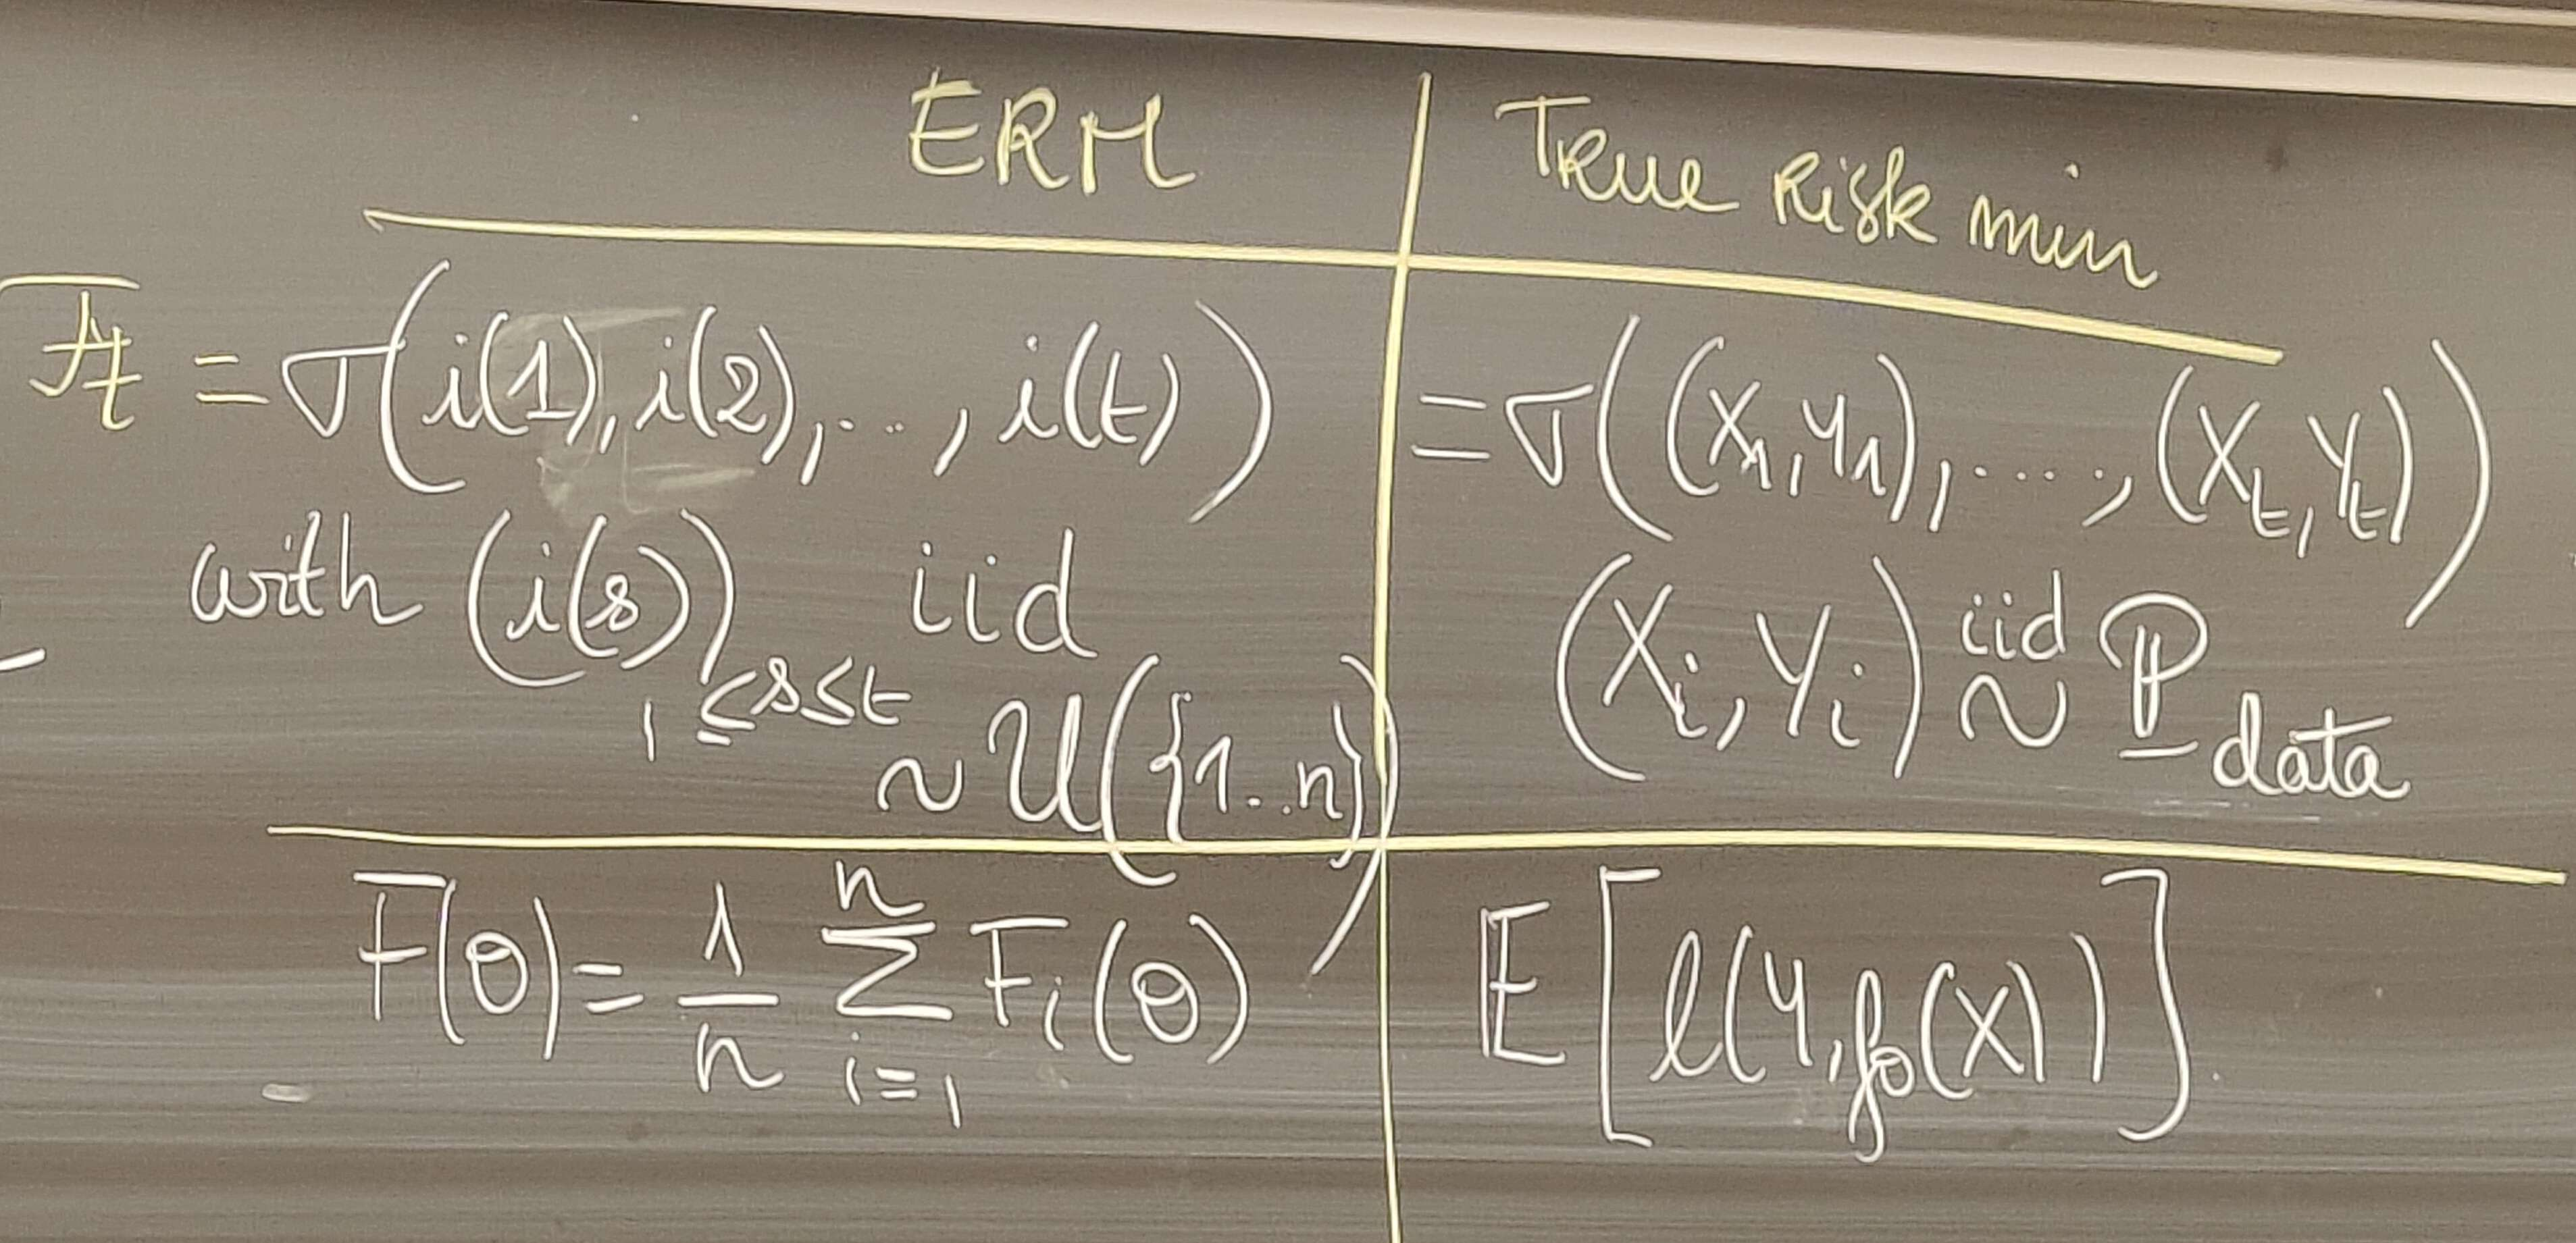
\includegraphics[width=.5\textwidth]{figs/thm_F_t.jpg}
    \caption{More explaination of $ \mathcal{F}_t $ }
    \label{explaination}
\end{figure}

\begin{note}
    \begin{itemize}
        \item 2 terms \begin{itemize}
            \item optimization term$\frac{\left\| \theta _0 - \theta ^\star  \right\|  ^2}{ 2 \gamma ( 1 - \frac{\gamma ^2}{2} ) T }$ similar to that of GD int the smooth case 
            \item The variance term $ \frac{\gamma  \sigma ^2}{2} $ impact of the noise which increase with $ \gamma  $ and $ \sigma ^2 $ 
        \end{itemize}
        
        \item Behaviour w.r.t $ \gamma  $ \begin{itemize}
            \item Because of optimisation : $ \frac{\left\| \theta _0 - \theta ^\star  \right\|  ^2}{ 2 \gamma ( 1 - \frac{\gamma ^2}{2} ) T } $ it goes up
            \item Bacause of Variance term : $ \frac{\gamma  \sigma ^2}{2} $ it goes down
        \end{itemize}
        
        \item Best trade-off is for $ \gamma \approx \frac{\left\| \theta _0 - \theta ^\star  \right\| }{4L \sqrt[]{T} \sigma } $ (constant step size but depending on the finit horizon)
        \item Comment the assumptions in the case ERM 
        \[
            F(\theta ) = \frac{1}{n} \sum_{i=1}^{n} F_i(\theta )
        .\]
        (ii) is satisfied whenever $ \forall t \geq 1, g_t = \nabla F_{i(t)} $ with $ i(t) \sim \mathcal{U}(\{1, \dots, n\})  $. \\
        Assume that (iii) holds for $ g_t = \nabla F_{i(t)} $ (usual SGD). \\
        One my use as gradient estimates $ g_t^{\left| B \right| } = \frac{1}{\left| B \right| } \sum_{i \in B_t} \nabla F_i$ where $ B_t $ is of cardinality $ \left| B_t \right| = \left| B \right|  $ uniformly ddrawn at random in $ \{ 1, \dots, n \} $  \\
        This is called a  \textbf{mini batch strategy}
        \begin{align*}
            \mathbb{E} [\left\| g_t^{\left| B \right| } (\theta ) - \nabla F(\theta)  \right\| ^2_2| \mathcal{F}_{t-1} ]
                &= \mathbb{E}[ \left\| \frac{1}{\left| B \right| } \sum_{i \in B_t}^{} \nabla F_i (\theta )  \right\| _2 ^2 | \mathcal{F}_{t-1} ] \\
                &= \mathbb{E}[ \left\| \frac{1}{\left| B \right| } \sum_{i \in B_t}^{} ( \nabla F_i (\theta ) - \nabla F(\theta )) \right\| _2 ^2 | \mathcal{F}_{t-1}] \\
                &= \frac{1}{\left| B \right|^2 } \left| B \right| \sigma ^2 = \frac{\sigma ^2}{\left| B \right| }
        \end{align*}
    \end{itemize}
\end{note}

\begin{proof}
    \[
        \left\| \theta _{t+1} - \theta ^{\star } \right\|^2_2 = \left\| \theta _{t} - \theta ^{\star } \right\|^2 - 2 \gamma _t \left\langle g_{t+1 }(\theta _t), \theta _t - \theta ^\star  \right\rangle + \gamma _t ^2 \left\| g_{t+1}(\theta _t) \right\| _2 ^2
    .\]
    Appying $ \mathbb{E}[ -1 \mathcal{F}_t] $ gives 
    \[
        \mathbb{E}[\left\| \theta _{t+1} - \theta ^\star  \right\| _2 ^2 | \mathcal{F}_t] = \left\| \theta _t - \theta ^\star  \right\| _2 ^2 - \mathbb{E}[2 \gamma _t \left\langle \nabla F(\theta _t), \theta _t - \theta ^\star  \right\rangle | \mathcal{F}_t] + \gamma _t ^2 \mathbb{E}[ \left\| g_{t+1} (\theta _t) \right\| _2 ^2 | \mathcal{F}_t]
    .\]
    $\left\| \theta _t - \theta ^\star  \right\| _2 ^2$ is $\mathcal{F}_t$-mesurable. and $\mathbb{E}[-2 \gamma _t \left\langle \nabla F(\theta _t), \theta _t - \theta ^\star  \right\rangle | \mathcal{F}_t] = -2 \gamma _t \left\langle \mathbb{E}[\nabla F(\theta _t)| \mathcal{F}_t], \theta _t - \theta ^\star  \right\rangle  = -2 \gamma _t \left\langle g_{t+1 }(\theta _t), \theta _t - \theta ^\star  \right\rangle  $ as $\theta _t - \theta ^\star  $ is $\mathcal{F}_t$-mesurable and with (ii).
    
    
    \begin{align*}
        \gamma _t ^2 \mathbb{E}[ \left\| g_{t+1} (\theta _t) \right\| _2 ^2 | \mathcal{F}_t] 
            &= \gamma _t ^2 \mathbb{E}[ \left\| g_{t+1} (\theta _t) - \nabla F(\theta _t) + \nabla F(\theta _t) \right\| _2 ^2 | \mathcal{F}_t ] \\
            &= \gamma _t ^2 \mathbb{E} [ \left\| g_{t+1}(\theta _t) - \nabla F(\theta _t) \right\| _2 ^2 | \mathcal{F}_t ] + \gamma _t ^2 \left\| \nabla F(\theta _t) \right\| _2 ^2 + 2 \gamma _t ^2 \left\langle \mathbb{E}[g_{t+1}(\theta _t) | \mathcal{F}_t ] - \nabla F(\theta _t), \nabla F(\theta _t) \right\rangle \\
            &= \gamma _t ^2 \mathbb{E} [ \left\| g_{t+1}(\theta _t) - \nabla F(\theta _t) \right\| _2 ^2 | \mathcal{F}_t ] + \gamma _t ^2 \left\| \nabla F(\theta _t) \right\| _2 ^2 + 2 \gamma _t ^2  * 0 \text{ not sure it's what she mean}\\
            &\leq \gamma _t ^2 \sigma ^2 + \gamma _t \left\| \nabla F (\theta _t) \right\| _2 ^2 \\
            &\leq \gamma _t ^2 \sigma ^2 + \gamma _t ^2 L \left\langle \nabla F(\theta _t) , \theta _t - \theta ^\star  \right\rangle \\
            & \text{ by cocoercivity of the gradient } \nabla F
    \end{align*}
    We get 
    \[
        \mathbb{E}[ \left\| \theta _{t+1} - \theta ^\star  \right\| _2 ^2 | \mathcal{F}_t] \leq \left\| \theta _t - \theta ^\star  \right\| _2 ^2 + ( -2 \gamma _t + \gamma _t ^2 L ) \left\langle \nabla F(\theta _t) , \theta _t - \theta ^\star  \right\rangle + \gamma _t ^2 \sigma ^2
    .\]
    By convexity of $ F $, 
    \begin{align*}
        F(\theta ^\star ) &\geq F(\theta e_t) + \left\langle \nabla F(\theta _t)  , \theta ^\star - \theta _t \right\rangle \\
        \text{i.e. } F(\theta _t) F^\star &\leq \left\langle \nabla F(\theta _t) , \theta _t - \theta ^\star  \right\rangle 
    \end{align*}
    If $ \gamma _t = \gamma \leq 1/L $, then 
    \begin{align*}
        0 \leq  \gamma _t L \leq 1 \\
        -2 \leq  -2 + \gamma _t L \leq  -1 \\
        -2 \gamma _t + \gamma _t ^2 L \leq - \gamma _t
    \end{align*}
    Therefore 
    \[
        \gamma \mathbb{E}[ F(\theta _t ) - F^\star ] \leq \mathbb{E}b[ \left\| \theta _t - \theta ^\star  \right\| _2 ^2] - \mathbb{E} [ \left\| \theta _{t+1} - \theta ^\star  \right\| _2 ^2 ] + \gamma ^2 \sigma ^2
    .\]
    Using Jensen's inequality, $ F(\bar{\theta _T}) = \frac{1}{\gamma T} \sum_{t=1}^{T} F(\theta _t) $. \\   
    Finaly 
    \[
        \mathbb{E}[F (\bar{\theta }_T - F^\star )] \leq \frac{1}{T}\sum_{t=1}^{T}\mathbb{E}[F(\theta _t) - F^\star ] \leq \frac{1}{\gamma T} \left\| \theta _0 - \theta ^\star  \right\| _2 ^2 + \gamma ^2 \sigma ^2
    .\]
\end{proof}
\begin{thm}[]
    F $\mu$-strongly cvx $L$-smooth. Ball $"\kappa = L/ \mu "$ \\
    Choose $\gamma _t = \begin{cases}
        \frac{1}{2L} &\text{ for } t \leq 4 \left\lceil \kappa  \right\rceil \\
        \frac{2t+1}{(t+1)^2 \mu} &\text{ for } t > 4 \left\lceil \kappa  \right\rceil \\
    \end{cases} $

    If $ t \geq 4 \left\lceil \kappa \right\rceil  $ , then 
    \[
        \mathbb{E}[\left\| \theta _t - \theta ^\star  \right\| _2 ^2 ] \leq \frac{\sigma ^2 4}{\mu t} + \frac{16 \left\lceil \kappa  \right\rceil ^2 }{c t^2} \left\| \theta _0 - \theta ^\star  \right\| _2 ^2
    .\]
    
\end{thm}

\begin{proof}[Proof:]
    See [Gower. ] 2014 / 2016. 
    
    TD : In the case $ \mu  $ -strongly convex \begin{itemize}
        \item $ \gamma = \frac{2}{\mu (t+1)} $
        \item $ \left\| g_t (\theta ) \right\| \leq b $  a.s. $ \forall \theta  $ 
        \item $ \theta _t = proj_B (\theta _{t-1} - \gamma _t g_t (\theta _{t-1})) $ 
    \end{itemize}
\end{proof}

\begin{note}[]
    \begin{itemize}
        \item \textbf{Good: } The result hold for the objective fonction 
        \[
            F(\theta ) - F(\theta ^\star ) \leq \left\langle \nabla F(\theta ^\star ), \theta - \theta ^\star  \right\rangle  + \frac{L}{2} \left\| \theta - \theta ^\star  \right\| _2 ^2 
        .\]
        \[
            \mathbb{E}[\left\| \theta _t - \theta ^\star  \right\| _2 ^2] = O(1/t) \Rightarrow \mathbb{E}[F(\theta _t) - F^\star ] = O(1/t)
        .\]
        
        \item \textbf{Bad: } With this proof strategy, we do not see the benefit of P-R averaging
        \[
            \mathbb{E}[F ( \bar{\theta}_T ) - F^\star ] \leq \frac{1}{T} \mathbb{E}[ \sum_{t=1}^{T} F(\theta _t) - F^\star ] \leq 0(\frac{\log_{} T  }{T})
        .\]
    \end{itemize}
\end{note}

We have proven this 
\begin{thm}[]
    $F$ smooth, unbiased gradients, uniformly bounded variance    
    \[
        \mathbb{E}[F(\bar{\theta }_T) - F^\star ] \leq \frac{\left\| \theta _0 - \theta ^\star  \right\| _2 ^2 }{\gamma T} + \gamma \sigma ^2 
    .\]
    For $ \gamma \propto 1 / \sqrt[]{T} $ 
    \[
        = O (1 / \sqrt[]{T})
    .\]
\end{thm}

\[
    \mathbb{E}[F({\theta }_t) - F^{\star} ] \leq \frac{1}{\gamma T} \left\| \theta _0 - \theta^{\star } \right\|^2 + \gamma  \sigma ^2 
.\]


\paragraph*{Exercice}
TD : In the case $ \mu  $ -strongly convex \begin{itemize}
    \item $ \gamma = \frac{2}{\mu (t+1)} $
    \item $ \left\| g_t (\theta ) \right\| \leq b $  a.s. $ \forall \theta  $ 
    \item $ \theta _t = proj_B (\theta _{t-1} - \gamma _t g_t (\theta _{t-1})) $ 
\end{itemize}

\paragraph*{Exercice 1 - TD3}
\begin{enumerate}
    \item \begin{align*}
        \left\| \theta _t - \theta ^\star  \right\| _2 ^2 
            &= \left\| proj_B (\theta _{t-1} - \gamma _t g_t (\theta _{t-1})) - \theta ^\star  \right\| _2 ^2 \\
            &= \left\| proj_B (\theta _{t-1} - \gamma _t g_t (\theta _{t-1})) - proj_B(\theta ^\star ) \right\| _2 ^2 \\
            &\leq \left\| \theta _{t-1} - \gamma _t g_t(\theta _{t - 1}) - \theta ^\star \right\| _2 ^2 \\
            &= \left\| \theta _t - \theta  ^\star  \right\| _2 ^2 + \gamma _t ^2 \left\| g_t(\theta _{t-1}) \right\| _2 ^2 - 2 \gamma _t \left\langle g_t(\theta _{t-1}), \theta _{t-1} - \theta ^\star  \right\rangle \\
        \mathbb{E}[ \left\| \theta _t - \theta ^\star  \right\| _2 ^2 | \mathcal{F}_{t-1}] 
            &\leq \mathbb{E}[\left\| \theta _{t-1} - \theta ^\star  \right\| _2 ^2 + \gamma _t ^2 \left\| g_t (\theta _{t-1} ) \right\| _2 ^2 - 2 \gamma _t \left\langle g_t(\theta _{t-1} ), \theta _{t-1} - \theta ^\star  \right\rangle | \mathcal{F}_{t-1}]
            &\leq \left\| \theta _{t-1} - \theta ^\star  \right\| _2 ^2 + \gamma _t ^2 b^2 - 2 \gamma _t \left\langle \nabla F(\theta _{t-1}), \theta _{t-1} - \theta ^{\star } \right\rangle 
    \end{align*}
    
    \item By $ \mu  $ - strong convex, $ F(y) - F(x) \geq \left\langle \nabla F(x) , y - x \right\rangle + \frac{\mu }{2} \left\| y - x \right\| _2 ^2, \forall x,y  $ \\
    for $x = \theta_{t-1}$ and $y = \theta ^{\star }$,
    
    \[
        F(\theta_{t-1}) - F(\theta ^{\star }) \leq \left\langle \nabla F(\theta_{t-1}) , \theta_{t-1} - \theta ^{\star } \right\rangle + \frac{\mu }{2} \left\| \theta_{t-1} - \theta ^{\star } \right\| _2 ^2
    .\]
    \begin{enumerate}
        \item $ \leq \frac{1}{2 \gamma _t } \left\| \theta _{t-1} - \theta ^\star  \right\| _2 ^2 + \frac{\gamma + b^2}{2} - \frac{1}{2 \gamma _t} \mathbb{E}[ \left\| \theta _t - \theta  ^\star  \right\| _2 ^2 | \mathcal{F}_{t-1}] - \frac{\mu }{2} \left\| \theta _{t-1} - \theta ^\star  \right\| _2 ^2 $ 
        \begin{align*}
            \mathbb{E}[F(\theta _{t-1} - F(\theta ^\star ))] 
                &\leq \frac{\mu (t+1)}{4} \mathbb{E}[\left\| \theta _{t-1} - \theta ^\star  \right\| ^2 ] + \frac{b^2}{ \mu (t+1)} - \frac{\mu (t+1)}{4} \left\| \theta _t - \theta ^star \right\| ^2 - \frac{\mu }{2} \mathbb{E}[\left\| \theta _{t-1 - \theta ^\star } \right\|^2] \\
            \mathbb{E}[F(\theta _{t-1}) - F(\theta ^\star )] 
                &\leq \frac{\mu (t-1)}{4} \mathbb{E}[\left\| \theta _{t-1} - \theta  ^\star  \right\|^2 ] - \frac{\mu (t+1)}{4} \mathbb{E}[\left\| \theta _t - \theta  ^\star  \right\| ^2 ] + \frac{b^2}{\mu (t+1)} \\
            \sum_{s=1}^{t}s \mathbb{E}[F(\theta _{s-1}) - F(\theta ^\star )] 
                &\leq \frac{\mu }{4} [\sum_{s=1}^{t} s (s-1) \mathbb{E}[\left\| \theta _{s-1} - \theta ^\star  \right\| _2 ^2] - s(s-1)\mathbb{E}[\left\| \theta _s - \theta ^\star  \right\| ^2]] + \frac{b^2}{\mu }t  \\
                &\leq \frac{b^2}{\mu }
        \end{align*}
        By convexity of F :
        \begin{align*}
            \mathbb{E}[F(\frac{2}{t(t+1)} \sum_{s=1}^{t} s \theta _{s-1}) - F(\theta ^{\star })] &\leq \frac{2}{t(t+1)} \sum_{s=1}^{t} s \mathbb{E}[F(\theta _{s-1}) - F(\theta ^{\star }) ]\\
            &\leq \frac{2}{t(t+1)} \sum_{s=1}^{t} s \mathbb{E}[F(\theta _{s-1}) - F (\theta ^\star )] \\
            &\leq \frac{2b^2}{\mu (t+1)}
        \end{align*}        
    \end{enumerate}
\end{enumerate}

\begin{note}[]
    \begin{itemize}
        \item L-smooth constant $ \gamma = mathcal{O}(1/\sqrt[]{T}) $, rate $ = mathcal{O}(1/\sqrt[]{T}) $ 
        \item L-smooth \& $ mu $-strongly convex, $ \gamma _t \propto \frac{1}{t} $ : rate $ = mathcal{O}(1/t) $ 
    \end{itemize}
    \begin{figure}[!h]
        \centering
        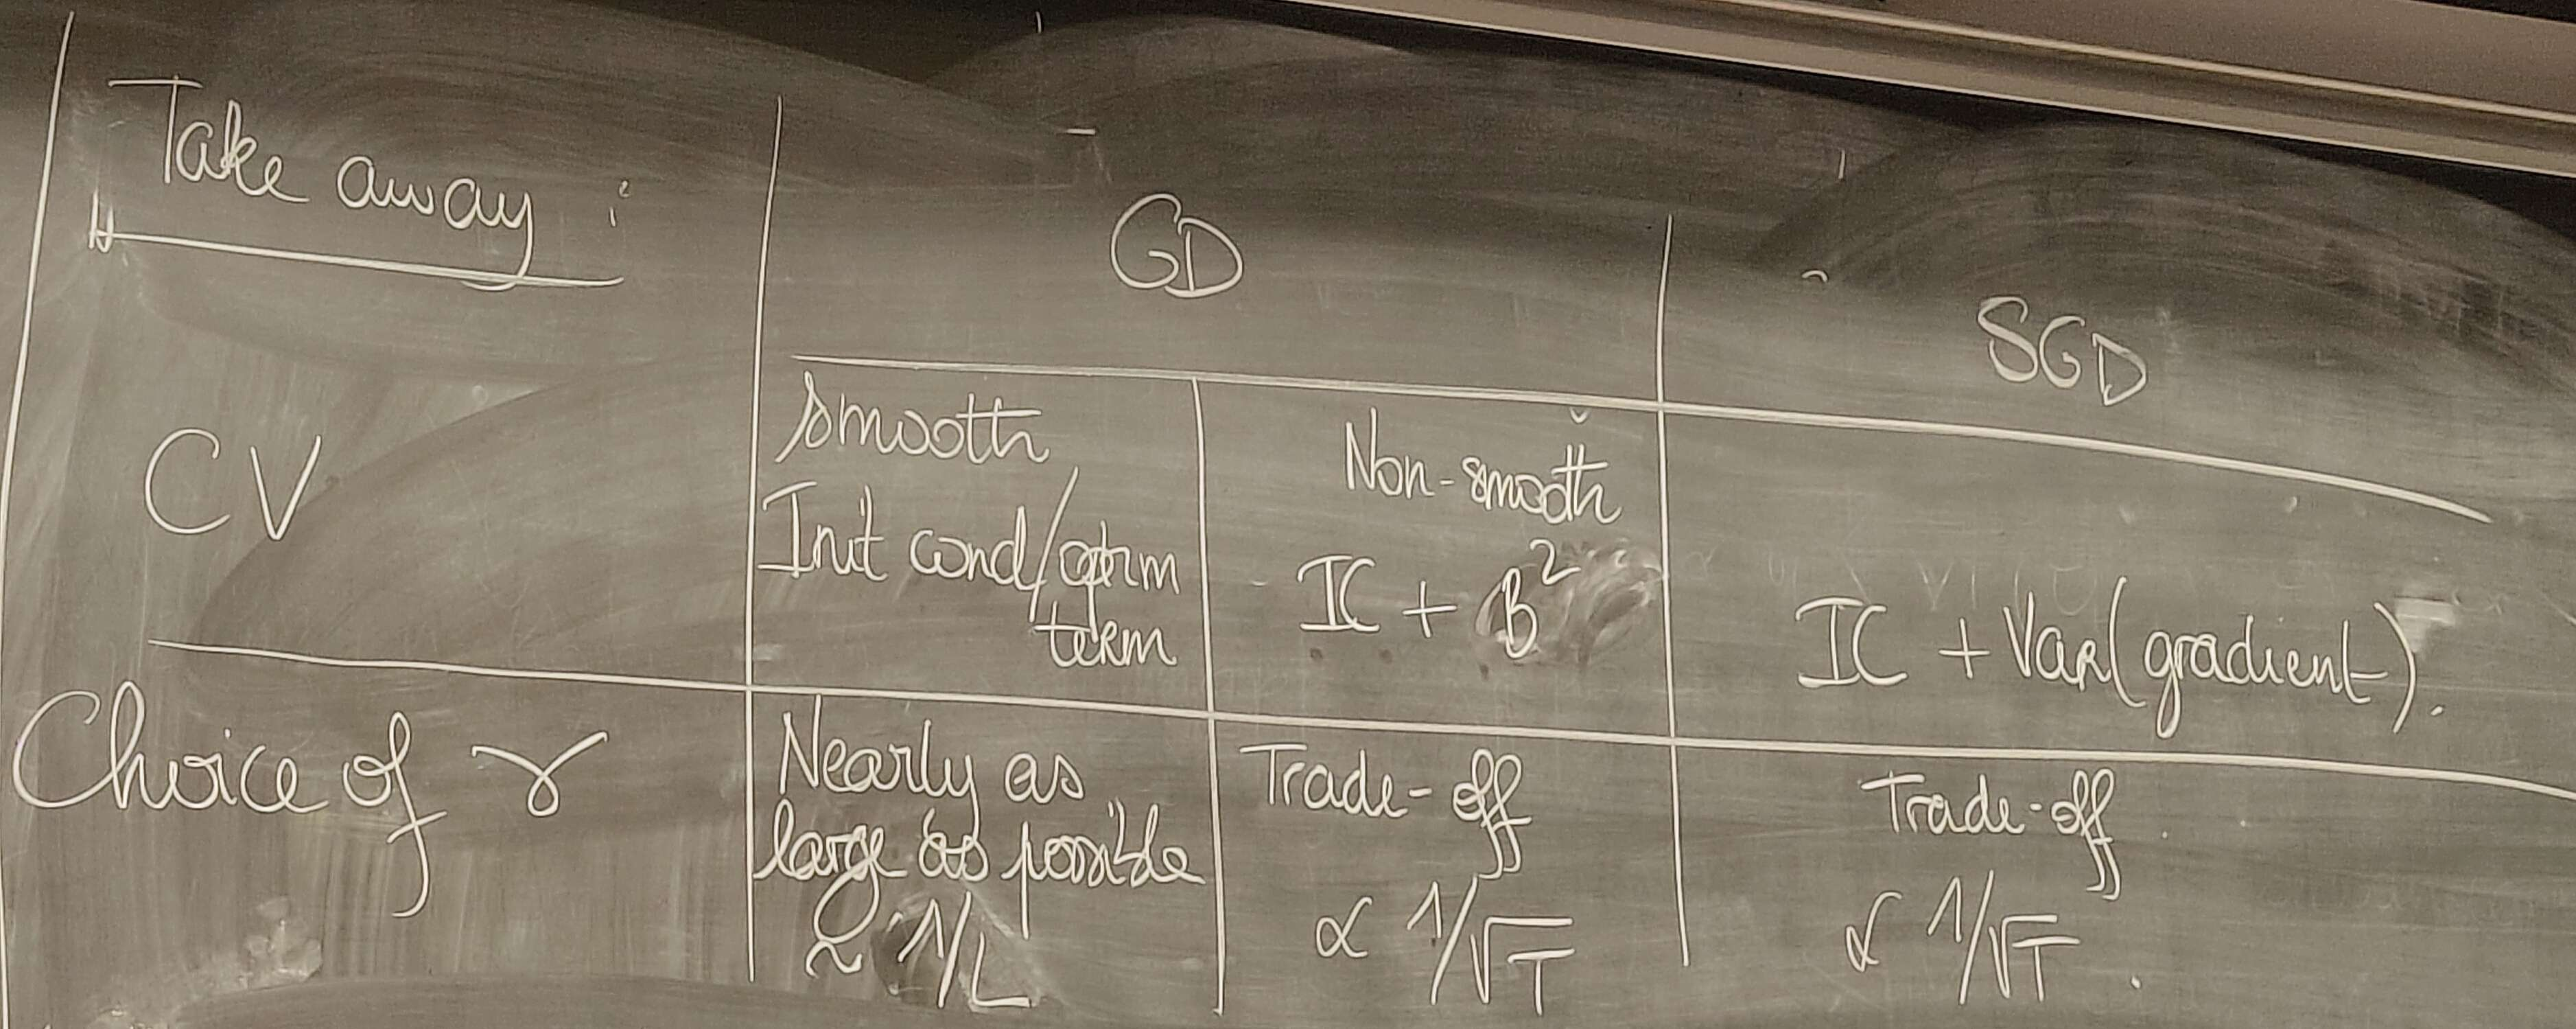
\includegraphics[width=.8\textwidth]{figs/take_away_table.jpg}
        \caption{Take Away table}
    \end{figure}

    \paragraph*{In terms of optimization, SGD vs GD : who is best?}
    Constext : $F$ smooth, ERM $F(\theta ) = \frac{1}{n} \sum_{i=}^{n} F_i(\theta )$
    \begin{figure}[!h]
        \centering
        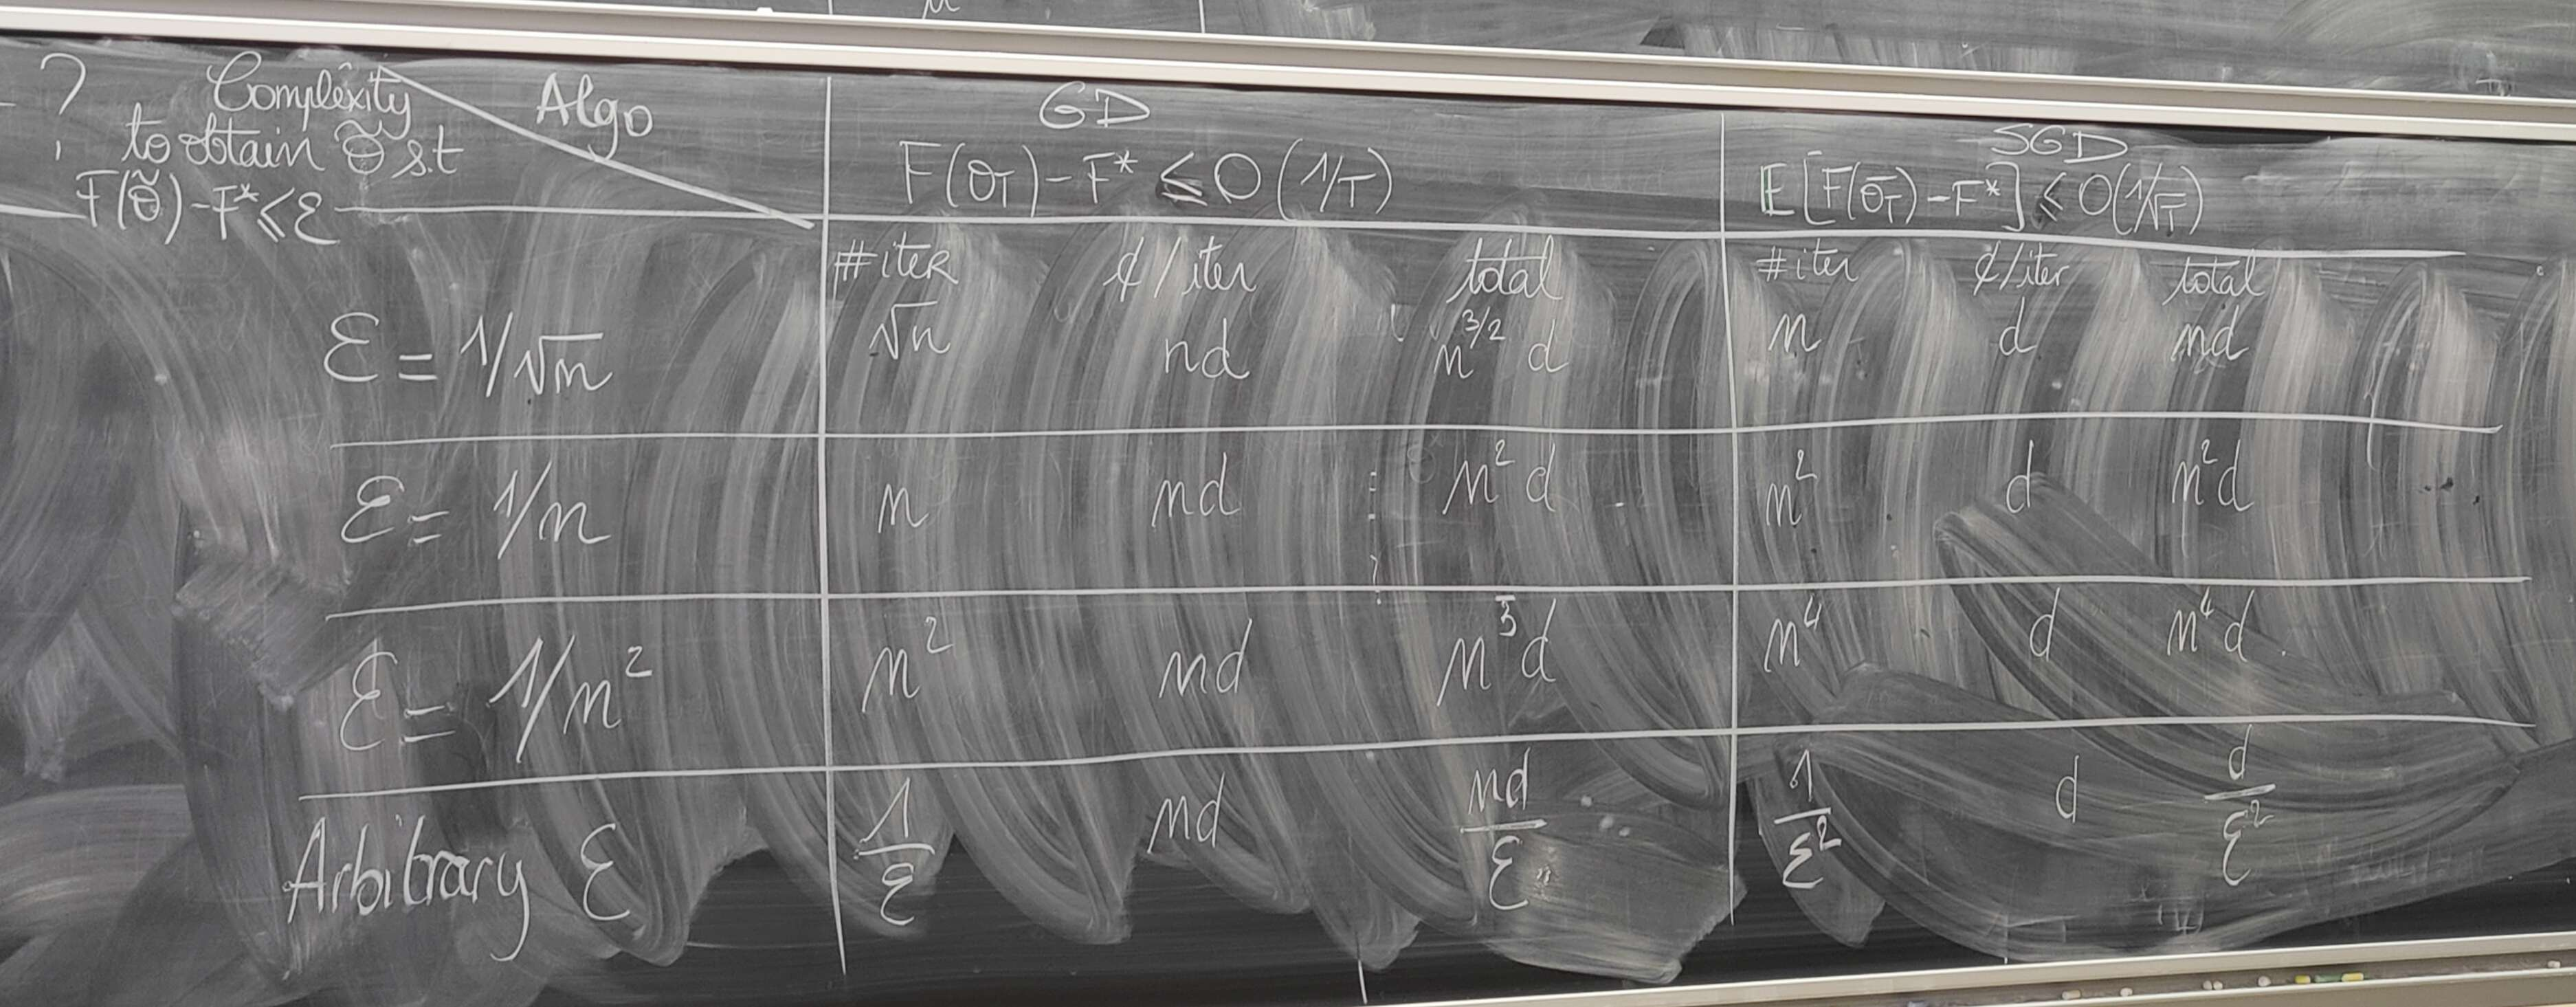
\includegraphics[width=.8\textwidth]{figs/SGD_vs_GD.jpg}
        \caption{In terms of optimization, SGD vs GD : who is best? }
    \end{figure}
    \begin{figure}[!h]
        \centering
        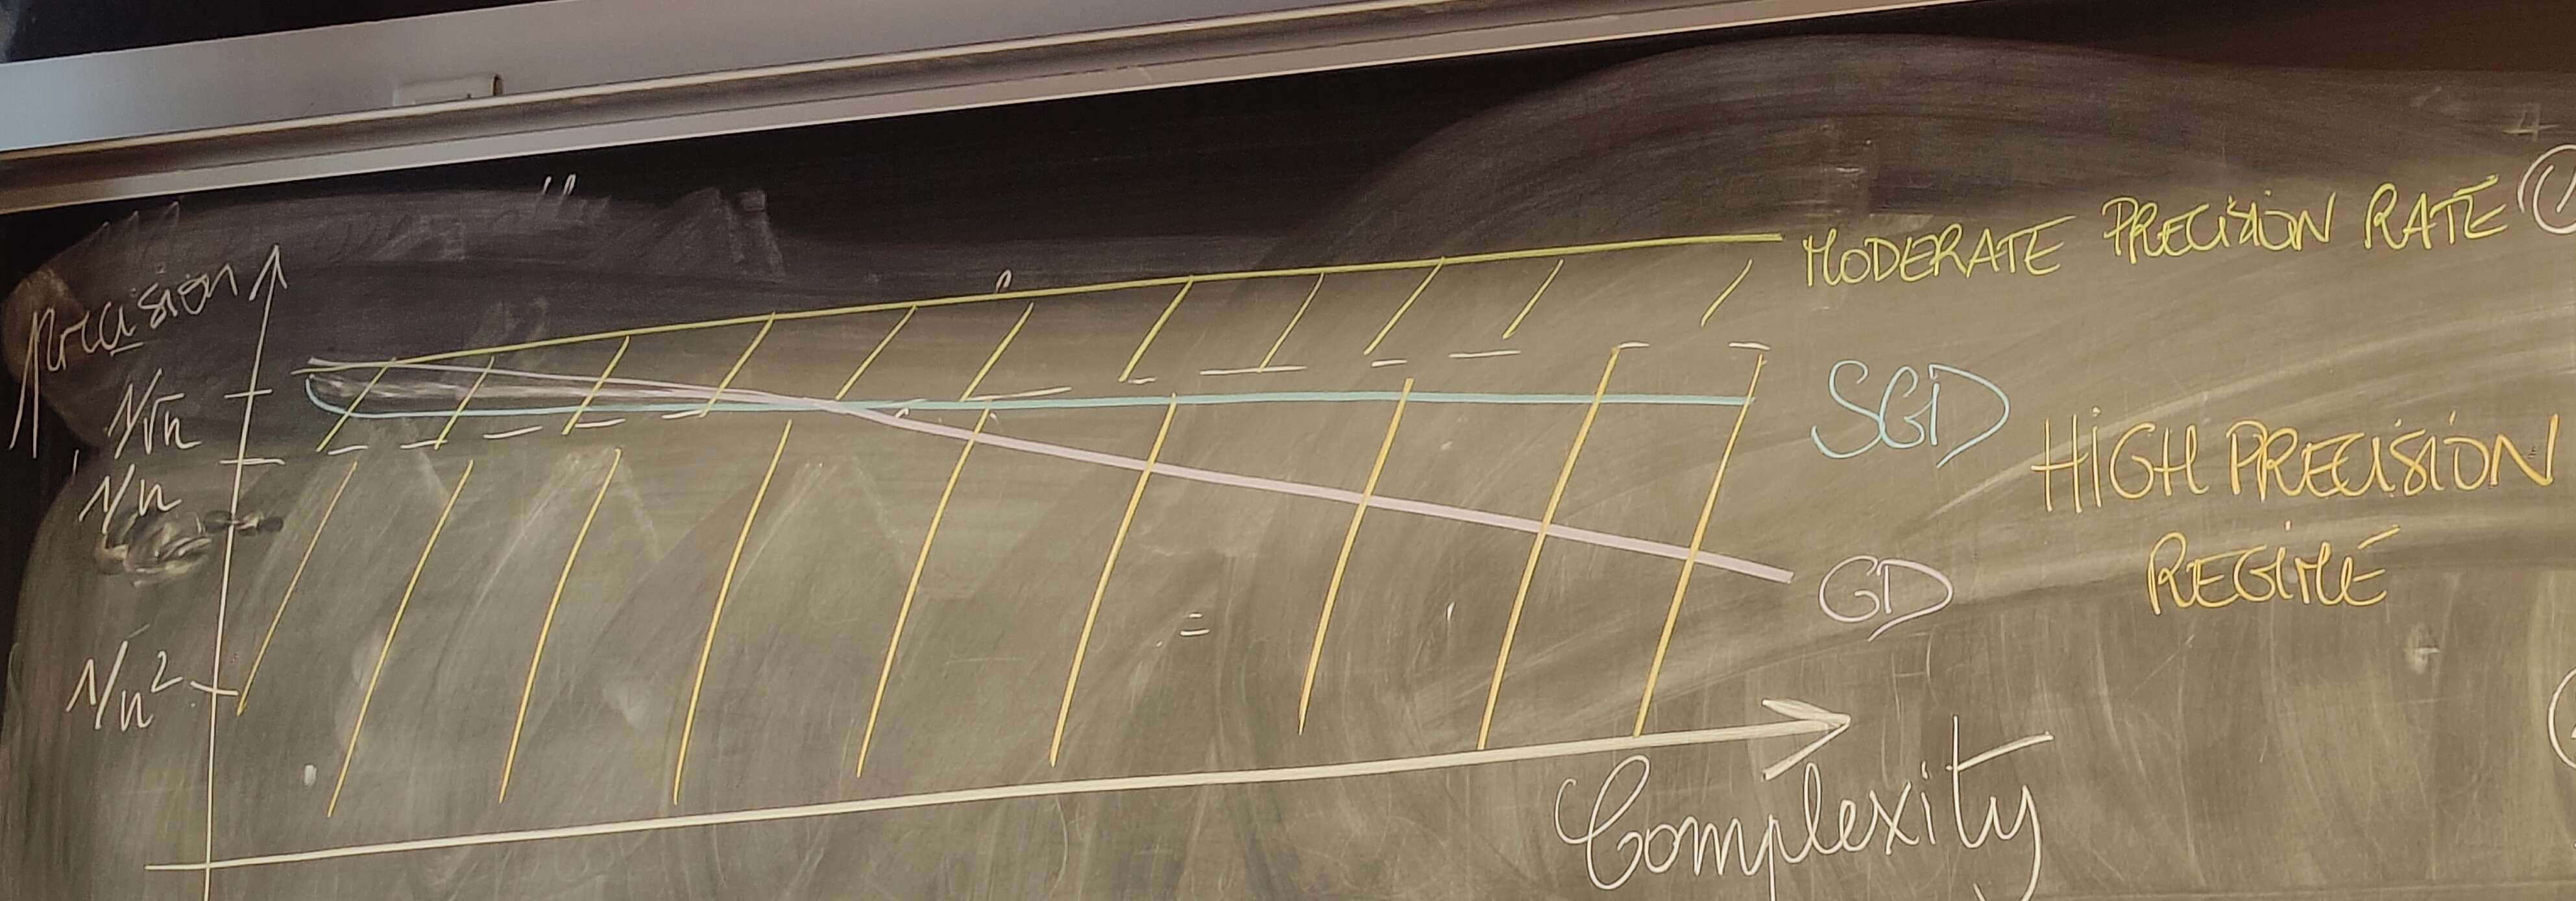
\includegraphics[width=.8\textwidth]{figs/SGD_vs_GD_graph.jpg}
        \caption{In terms of optimization, SGD vs GD : who is best? Graph }
    \end{figure}

    \begin{enumerate}
        \item GD tends to outperform SGD (in termes of complexity) for hig presion regimes
        \item SGD outperforms GD for low to moderate precision regimes
    \end{enumerate}
    So none is best. It depends to the precision. \\
    The frontier between "moderate" \& "high" precision has been fixed to $\frac{1}{n}$.
    In ML, one aims to optimize up to the \textbf{statistical} precision, ranging from $ 1 / \sqrt[]{n} $ to $ 1/n $, thus moderate precision is enough! \\
    
    \textbf{CCL}\begin{itemize}
        \item For optimization, no best method between GD and SGD
        \item For ML , moderate precision, better choose SGD
    \end{itemize}

    \paragraph*{In terms of generalization?}
    \begin{itemize}
        \item Running SGD for the expected risk minimization with $ n $ samples leads to a generatization error $ \propto 1/\sqrt[]{n} $. This has to be compared with classical bounds of stat/ML
        \begin{figure}[!h]
            \centering
            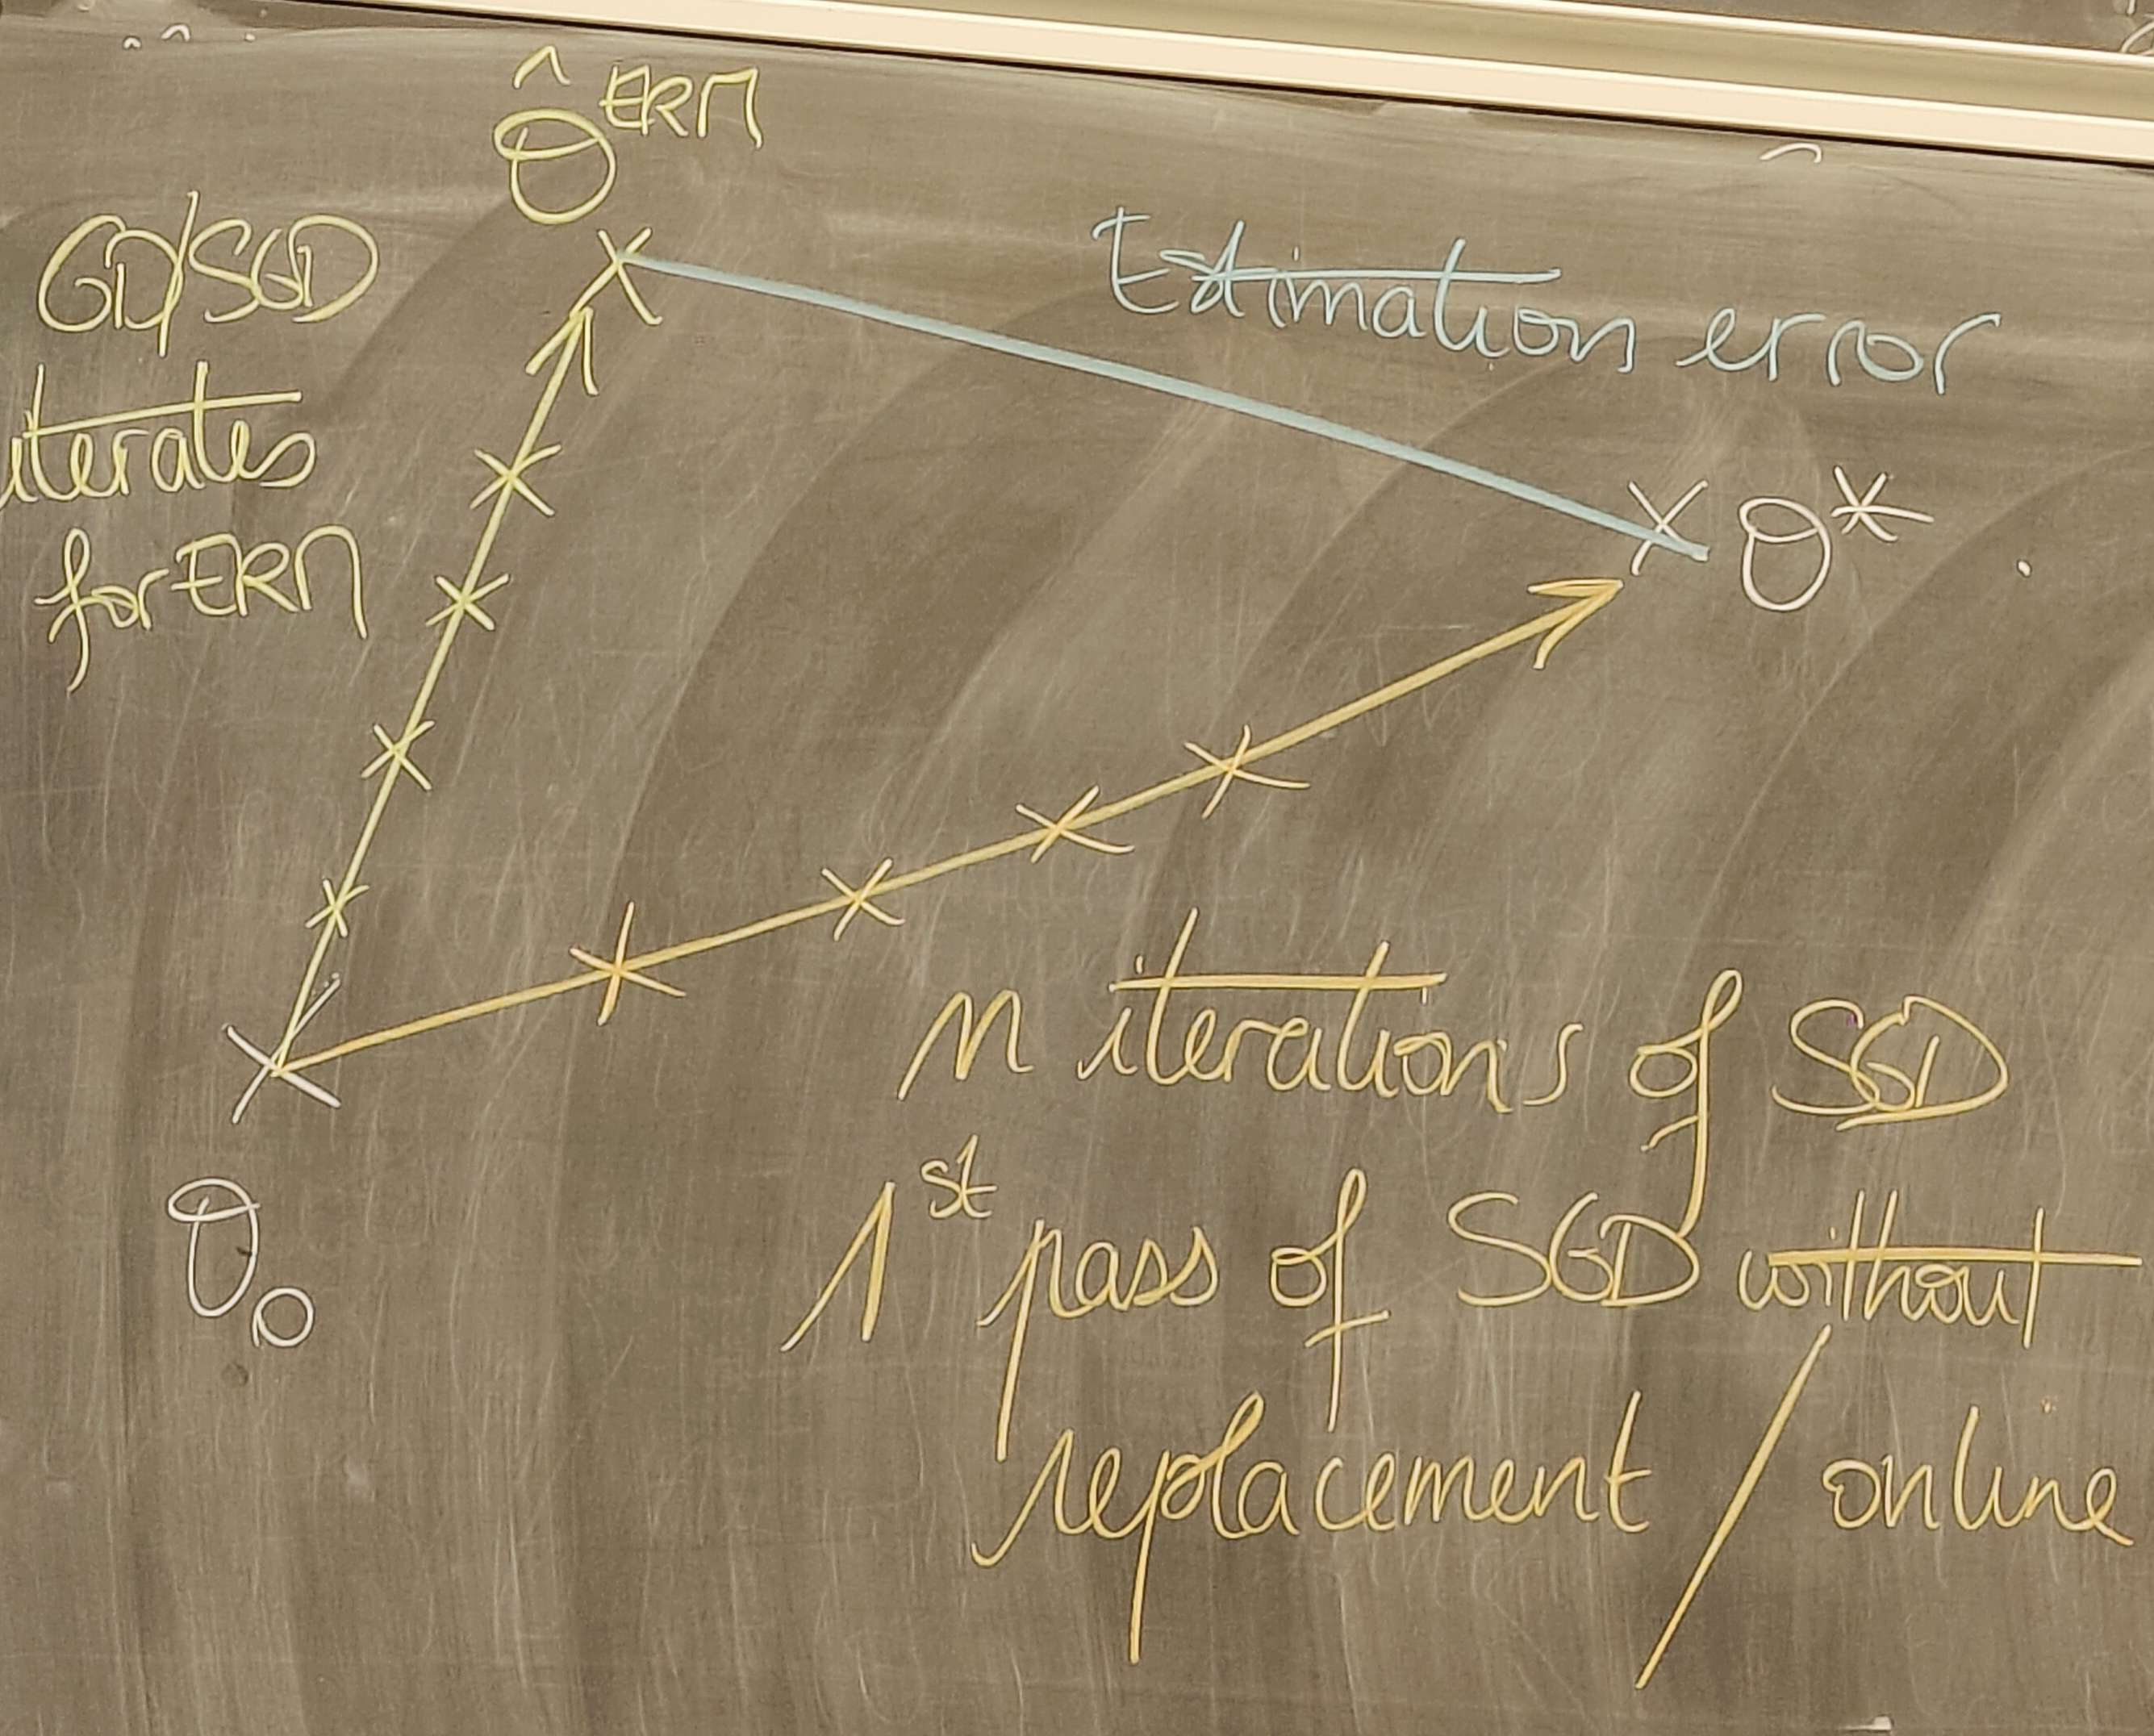
\includegraphics[width=.8\textwidth]{figs/SGD_vs_GD_generalization.jpg}
            \caption{In terms of optimization, SGD vs GD : who is best? Graph }
        \end{figure}
        SGD on the expected risk avoids estimation pb. One pass of SGD may be competitive without exact ERM. \\
        In term of running complexities, we get :
        \begin{align*}
            \mathcal{O} (tnd) = \mathcal{O}(n^2 d) &\text{ vs } \mathcal{O}(nd) \\
            (GD \text{ for } ERM) &\text{ vs } (SGD)
        \end{align*}
        \textbf{Warning} We are only comparing upperbounds!
        
    \end{itemize}
\end{note}






\underline{Nouveau cours du 30/11} \\

\begin{figure}[!h]
    \centering
    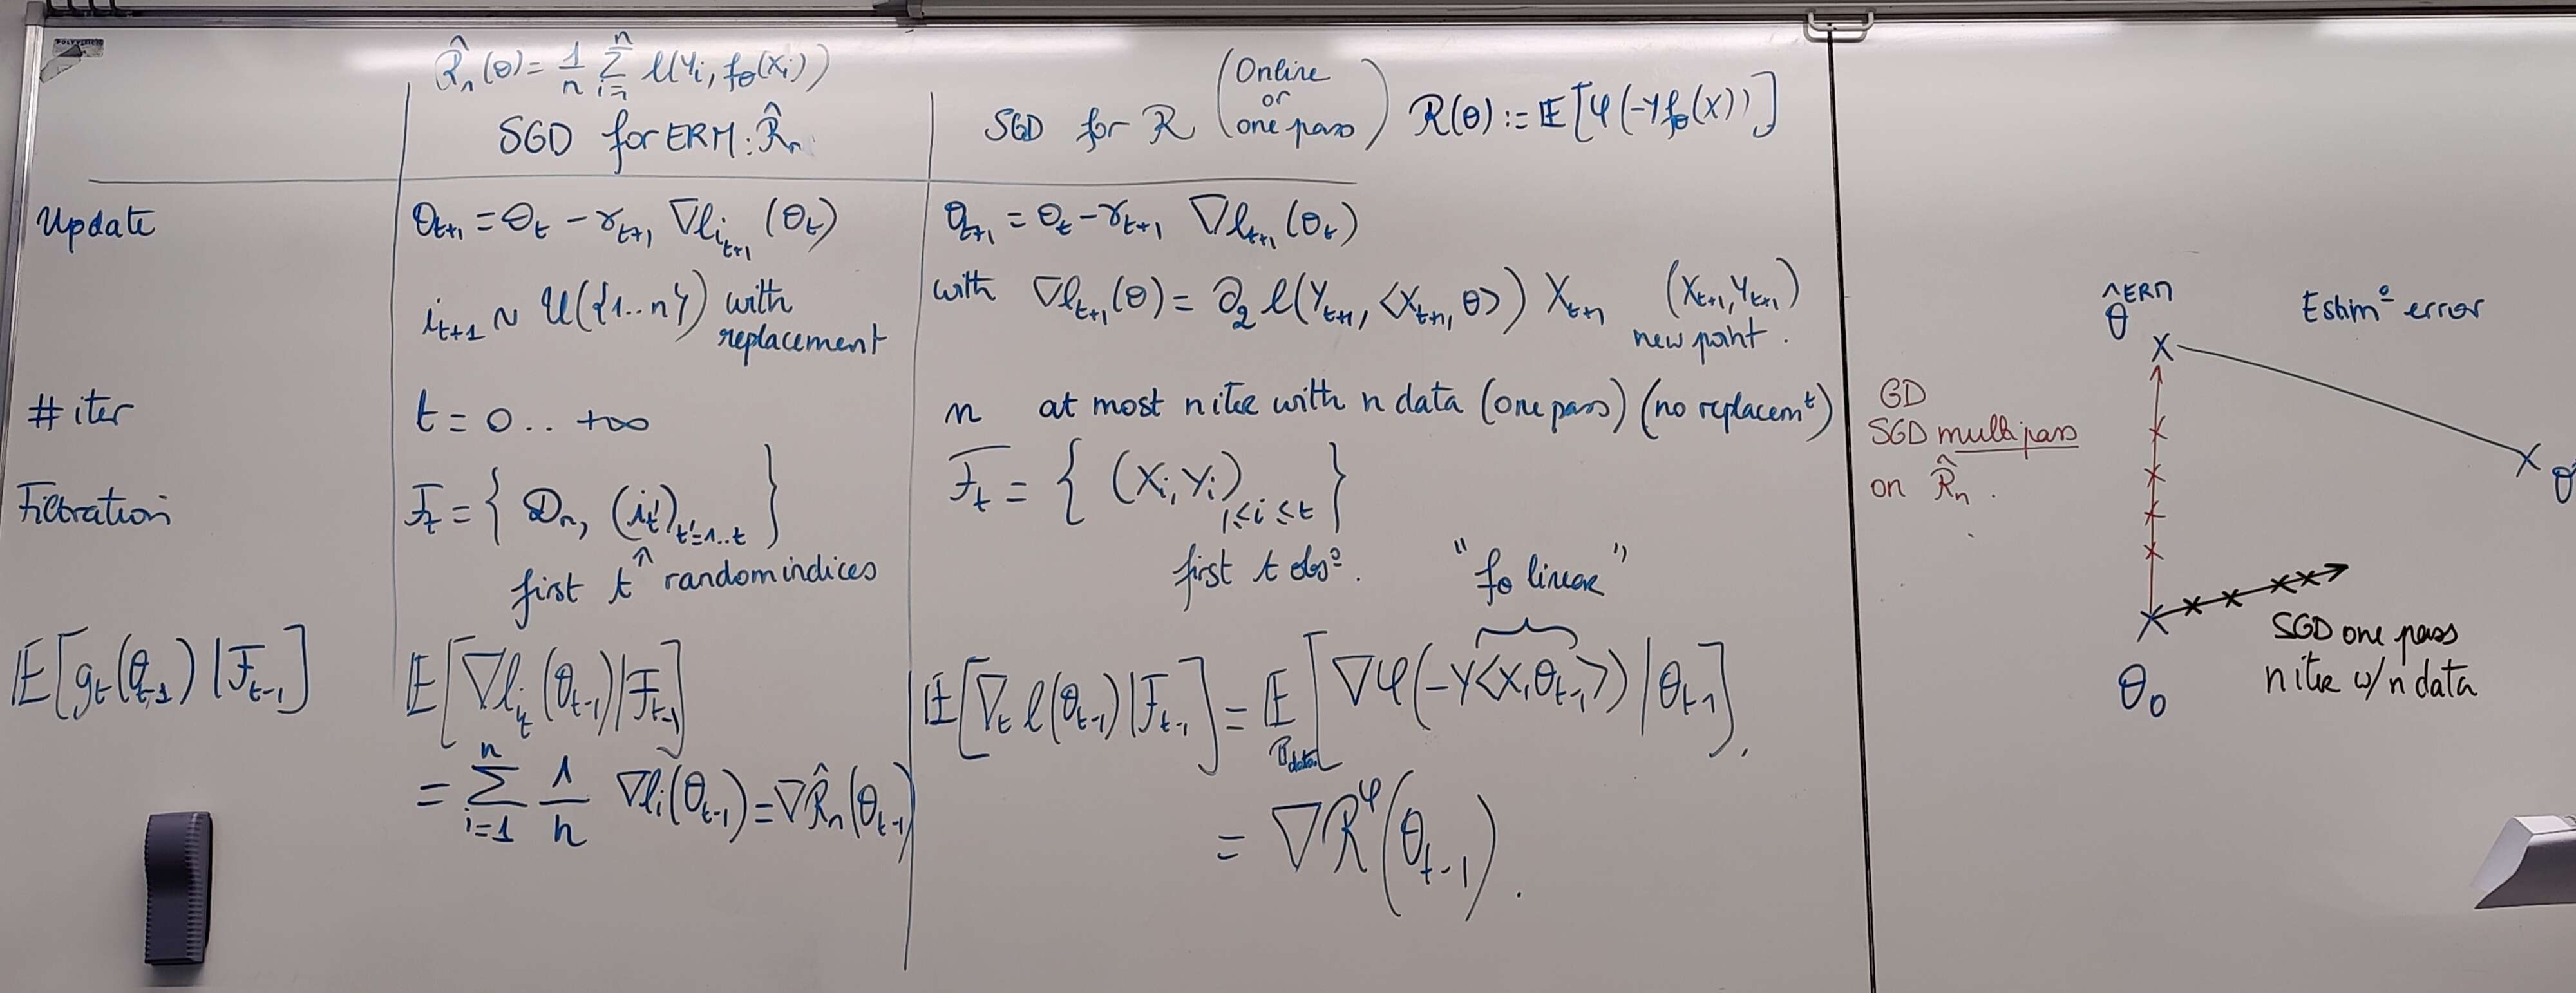
\includegraphics[width=.95\textwidth]{figs/sum_up_SGD_table.jpg}
    \caption{Comparaison between SGD for ERM $\hat{\mathcal{R}}_n$ and SGD for $\mathcal{R}$ }
\end{figure}

\textbf{Averaging} : In the case of strongly cvx fonction \& smooth
\begin{itemize}
    \item SGD with no averaging $ \gamma _t = Ct^{- \alpha }, \alpha =1 $
    \item SGD + averaging $ \gamma _t = C t^\alpha , \frac{1}{2} \leq \alpha \leq 1 $ rate : $ \mathcal{O} (t^{-1} \mu ^{-1} ) $ 
\end{itemize}

=> Averaging help in case of "bad choice" of step size. \\
\textbf{Take-home message} : use $\alpha  = \frac{1}{2}$ + averaging.


\chapter{Stability of learning Algorithm \& generalizations}

\section{Motivation}
\begin{figure}[!h]
    \centering
    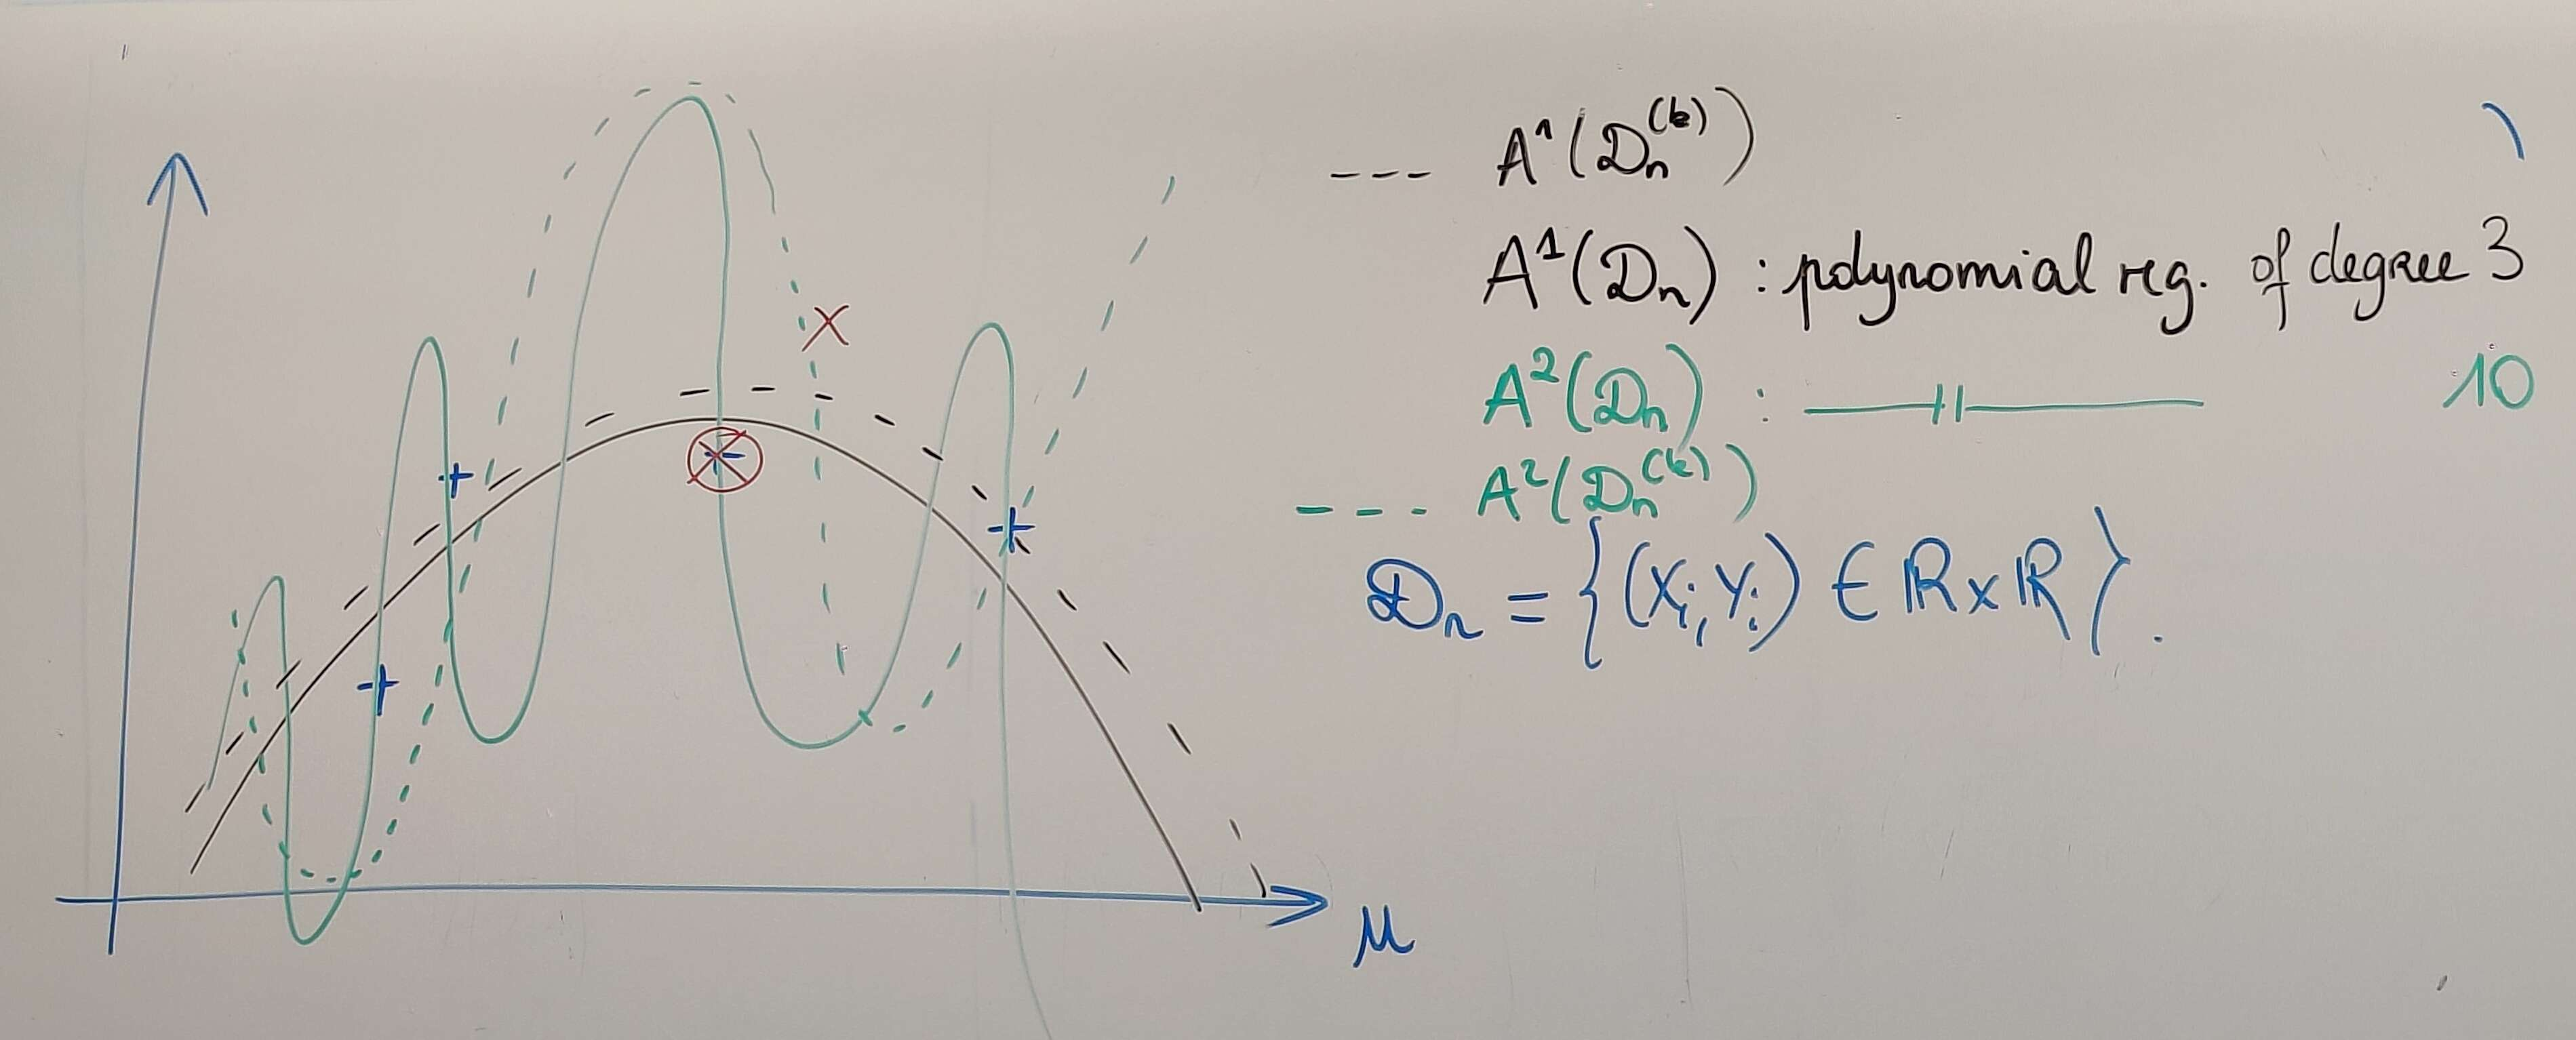
\includegraphics[width=.8\textwidth]{figs/chapter_4_motivation.jpg}
    \caption{Chapter 4: Motivation. The black algorythm seem better (better generalization, less overfitting) }
\end{figure}

\textbf{Generalization} : for a test point $(X, Y)$ of same distrib and $\ind $ of $\mathcal{D}_n$, evaluation of $\mathbb{E}[l(Y, A(\mathcal{D}_n)(X))]$

Another point of view of generalization : compare $ A(\mathcal{D}_n ) $ vs $ A(\mathcal{D}_n^{(k)}) $ where $ \mathcal{D} _n ^{(k)} $ is the training set in which we change the $ k $-th point.

\[
    \mathcal{D}_n^{(k) \leftarrow (X'_{k}, y'_{k} )} = {(X_1, Y_1) ... (X_{k-1}, Y_{k-1}),(x'_{k}, y'_{k}),(X_{k+1}, Y_{k+1}), ... (X_n, Y_n)}
.\]
In the picture  \begin{itemize}
    \item $ A^1 (\mathcal{D}_n) $ is "close" to $ A^1( \mathcal{D }_n ^{(k)}) $ 
    \item $ A^2 (\mathcal{D}_n) $ is very different from $ A^2( \mathcal{D }_n ^{(k)}) $ $\rightarrow A^2$  is unstable.
\end{itemize}
Claim : Stability implies generalization 

\begin{defn}[]
    A learning algo $(A_n)_n$ is a sequence of mapping
    \begin{align*}
        A_n : (\mathcal{X}&, \mathcal{Y})^{\times n} \to \mathcal{C} \\
                &\mathcal{D}_n \mapsto A_n (\mathcal{D}_n ) (\text{ possibly random})
    \end{align*}
    from any number of points into the set $\mathcal{C}$ of classifier.
\end{defn}

\begin{exmp}[1]
    Empirical risk minimizer over $ \Theta  $ is a learning algo 
    \[
        A^{ERM}(\mathcal{D}_n) \equiv \arg \min_{\theta \in \Theta}\hat{\mathcal{R}}_{n, \mathcal{D}_n }(\theta )
    .\]
    
\end{exmp}


\begin{exmp}[This is a \textbf{randomized algo}]
    SGD with T steps and $(\gamma _t)_{t=1...T}$ is a learning algo
    \[
        A^{SGD} \equiv \begin{cases}
            \theta _0 &= 0 \\
            \theta _{t+1} &= \theta _t - \gamma _{t+1} g_{t+1} (\theta _t) \text{ for } t = 0, \dots, T-1 \\
        \end{cases}
    .\]
    where $ g_t (\theta _{t-1} ) $ is the gradient of 
    \[
        \theta  \mapsto l(Y_{i_t} , \left\langle \theta , X_{i_t} \right\rangle ), i_t \sim \mathcal{U}(\{1, \dots, n\})
    .\]
    
\end{exmp}

\begin{defn}[Uniform stability (deterministic algo)]
    Concider a deterministic algo A \\
    A is uniformly stable for $ \beta : \mathbb{N} \to \mathbb{R}_+ $ if for \textbf{any} $\mathcal{D}_n$, for \textbf{any} $k$, for \textbf{any} $(X'_k, Y'_k) \in \mathcal{X} \times \mathcal{Y}$, for any test point $(X_{test}, T_{test}) \in \mathcal{X}, \mathcal{Y}$ 
    \[
        \left| l(Y_{test}, A(\mathcal{D}_n)(X_{test})) - l(Y_{test}, A(\mathcal{D}_n^{(k) \leftarrow (X'_{k}, Y'_{k} )})(X_{test})) \right| \leq \beta (n)
    .\]
    
\end{defn}

\begin{defn}[Uniform stability (randomized algo)]
    Concider a randomized algo A \\
    A is uniformly stable for $ \beta_{av} : \mathbb{N} \to \mathbb{R}_+ $ if for \textbf{any} $\mathcal{D}_n$, for \textbf{any} $k$, for \textbf{any} $(X'_k, Y'_k) \in \mathcal{X} \times \mathcal{Y}$, for any test point $(X_{test}, T_{test}) \in \mathcal{X}, \mathcal{Y}$ 
    \[
        \mathbb{E}[\left| l(Y_{test}, A(\mathcal{D}_n)(X_{test})) - l(Y_{test}, A(\mathcal{D}_n^{(k) \leftarrow (X'_{k}, Y'_{k} )})(X_{test})) \right|] \leq \beta_{av} (n)
    .\]
    Thi only random thing is the algo
\end{defn}

\begin{note}[]
    We could extend thses definitions to EXPECTED stability (kind of a less stronger version) : for $ (X_i, Y_i)_{i=1} ^n, (X_k^\prime , Y_k^\prime ), (X_{test}, Y_{test}) \sim \mathbb{P}_{data}^{\otimes (n+2)} $ 
\end{note}

\paragraph*{Ref} : \begin{itemize}
    \item Stability introduced in Bousquet \& Elisseeff (2002)
    \item Re-introduced by HArdt, Recht, Singer "Train faster, generalize bettter" (2016)
    \item Widely used since then
\end{itemize}

\begin{note}[]
    Related to algorithm sensibility, privacy-preserving algo with DP (differential privacy) \\
    \[
        (\epsilon , \delta ) \text{-DP} : \forall S, \mathbb{P}(A(\mathcal{D}_n) \in S) \leq (1+\epsilon ) \mathbb{P}(A(\mathcal{D}_n^{(k)}) \in S) + \delta 
    .\]
    $\leadsto $ Aurélien Bellet, french expert in Monpelier.
\end{note}

\section{Stability implies generalization}


\textbf{Warning}: A stupid algo A such that $ \forall \mathcal{D}_n, A(\mathcal{D_n}) = \theta _0 \ind \mathcal{D}_n $ is $ \beta $-stable for $ \beta = 0 $. \\

\textbf{Intuition}: the generalization ability should be controlled by : 1. Stability term ; 2. Data-fitting term. \\

\begin{lem}[]
    Call $ \theta ^\star  = \arg \min_{\theta  \in  \Theta } \mathcal{R}(\theta )$  and $\theta ^{ERM} = \arg \min_{\theta  \in  \Theta} \hat{\mathcal{R}}_{n, \mathcal{D}_n}(\theta )$
\begin{align*}
    \mathbb{E}[ \mathcal{R} (A (\mathcal{D}_n )) - \mathcal{R} (\theta ^\star )] \leq &\mathbb{E}[ \underbrace{\mathcal{R} (A (\mathcal{D}_n )) - \hat{\mathcal{R}} _{n, \mathcal{D}_n} (A (\mathcal{D}_n ))}_{\text{Difference between generalisation / empirical errors } \approx \text{Stability}}     ] \\
    & + \underbrace{\mathbb{E}[ \hat{\mathcal{R}}_{n, \mathcal{D}_n} (A (\mathcal{D}_n)) - \hat{\mathcal{R}}_{n ,\mathcal{D}_n} ( \hat{\theta }^{ERN })]}_{\text{optim error} \leadsto \text{ data fitting term}}
\end{align*}
\end{lem}

\begin{note}[]
    For any predictor $\theta _0 \ind \mathcal{D}_n $ 
    \[
        \mathcal{R}(\theta _0) = \mathbb{E}[\hat{\mathcal{R}}_{n, \mathcal{D}_n}(\theta_0 )]
    .\]
    
\end{note}

\begin{proof}[Preuve : ]
    \begin{align*}
        \mathcal{R}(A(\mathcal{D}_n)) - \mathcal{R}(\theta ^\star ) &= \mathcal{R}(A(\mathcal{D}_n)) - \hat{\mathcal{R}} _{n, \mathcal{D}_n} (A (\mathcal{D}_n )) \\
        &+ \hat{\mathcal{R}} _{n, \mathcal{D}_n} (A (\mathcal{D}_n )) - \hat{\mathcal{R}} _{n, \mathcal{D}_n} (\hat{\theta }^{ERM}) \\
        &+ \hat{\mathcal{R}} _{n, \mathcal{D}_n} (\hat{\theta }^{ERM}) - \hat{\mathcal{R}} _{n, \mathcal{D}_n} (\hat{\theta }^{\star }) \quad \textcolor{red}{\leq 0 \text{ since } \hat{\theta }^{ERM} \in \arg \min _{\Theta } \hat{\mathcal{R}} _{n, \mathcal{D}_n}}\\
        &+ \hat{\mathcal{R}} _{n, \mathcal{D}_n} (\hat{\theta }^{\star }) - \mathcal{R}(\theta ^\star ) \\
    \end{align*}
    And 
    \begin{align*}
        \mathbb{E}[\mathcal{R}(A(\mathcal{D}_n)) - \mathcal{R}(\theta ^\star )] &= \mathbb{E}[\mathcal{R}(A(\mathcal{D}_n)) - \hat{\mathcal{R}} _{n, \mathcal{D}_n} (A (\mathcal{D}_n )) ] \\
        &+ \mathbb{E}[\hat{\mathcal{R}} _{n, \mathcal{D}_n} (A (\mathcal{D}_n )) - \hat{\mathcal{R}} _{n, \mathcal{D}_n} (\hat{\theta }^{ERM}) ] \\
        &+ \mathbb{E}[\hat{\mathcal{R}} _{n, \mathcal{D}_n} (\hat{\theta }^{ERM}) - \hat{\mathcal{R}} _{n, \mathcal{D}_n} (\hat{\theta }^{\star }) ] \\
        &+ \mathbb{E}[\hat{\mathcal{R}} _{n, \mathcal{D}_n} (\hat{\theta }^{\star }) - \mathcal{R}(\theta ^\star )] \quad \textcolor{red}{=0 \text{ since } \theta ^\star \ind \mathcal{D}_n} \\
    \end{align*}
\end{proof}

\begin{note}[]
    For example 1, $ A(\mathcal{D}_n) \equiv \hat{\theta }^{ERN} $, Lemma 22 gives 
    \[
        \mathbb{E}[ \mathcal{R} (A (\mathcal{D}_n))] - \mathcal{R} (\theta ^\star ) \leq  \mathbb{E}[ \mathcal{R}(A(\mathcal{D}_n)) - \hat{\mathcal{R} } _{n, \mathcal{D}_n} ( A(\mathcal{D}_n)) ]
    .\]
    the optim error vanishes
\end{note}

\begin{thm}[Stability $\rightarrow$ Generalization]
    If A is a learning algo which is $ \beta  $-uniformly stable then 
    \[
        \mathbb{E}[ \mathcal{R}(A(\mathcal{D}_n)) - \hat{\mathcal{R}}_{n,\mathcal{D}_n}] \leq \beta (n)
    .\]
\end{thm}
\begin{proof}[Preuve : ]
    Reminder \begin{itemize}
        \item $ \mathcal{R} (A(\mathcal{D}_n)) = \mathbb{E}_{(X,Y) \sim p}[ l(Y, A(\mathcal{D}_n)) | \mathcal{D}_n] $ 
        \item $ \mathbb{E}_{\mathcal{D}_n} [ \mathcal{R}(A (\mathcal{D}_n))] $ 
        \item $ \hat{\mathcal{R}}_{n, \mathcal{D}_n} (A(\mathcal{D}_n)) = \frac{1}{n} \sum_{i=1}^{n } l (Y_i, A(\mathcal{D}_n) (X_i)) $ 
        \item $ \mathbb{E}_{\mathcal{D}_n} [ \hat{\mathcal{R}}_{n, \mathcal{D}_n}(A (\mathcal{D}_n))] $ 
    \end{itemize}
    Observe that for any $ k \in \{1, \dots, n\} $ 
    \begin{align*}
        \mathbb{E} [\mathcal{R}(A(\mathcal{D}_n))]
            &= \mathbb{E}_{ \mathcal{D}_n \sim p^{\otimes n} ,, \ind (X,Y)\sim p} [ l(Y, A (\mathcal{D}_n) (X)) ] \\
            &= \mathbb{E}_{ \mathcal{D}_n \sim p^{\otimes n} ,, \ind (X,Y)\sim p} [ l(Y_k, A(\mathcal{D}_n^{(k)}) (X_k))]
    \end{align*}
    Since $ ( (X_1, Y_1), \dots, (X_k, Y_k), \dots, (X_n, Y_n), (X,Y) ) = ^{\text{dist}} ( (X_1, Y_1), \dots, (X, Y) \dots, (X_n, Y_n), (X_k,Y_k) )$ 

    Therefore
    \begin{align*}
        \mathbb{E} [\mathcal{R}(A(\mathcal{D}_n)) - \hat{\mathcal{R}}_{n, \mathcal{D}_n} (A(\mathcal{D}_n))] 
            &= \mathbb{E}[ \frac{1}{n} \sum_{k=1}^{n} ( \mathcal{R} (A ( \mathcal{D}_n) ) - l ( Y_k, A(\mathcal{D}_n) (X_k)))] \\
            &= \frac{1}{n} \sum_{k=1 }^{n} \mathbb{E}[ \underbrace{l( Y_k, A(\mathcal{D}_n ^{(k) (X,Y) })(X_k) ) -l (Y_k , A(\mathcal{D}_n) (X_k))}_{ \leq \beta (n) \text{ by stability assumption}} ] \\
            &\leq \beta (n)
    \end{align*}
\end{proof}

\textbf{CCL} : 
\begin{itemize}
    \item (BEFORE) $ gen \leq \underbrace{\text{state rate}}_{\text{Worst } \hat{\mathcal{R}}_n - \mathcal{R} \text{ on } \theta \in \Theta ( \text{ Uniform bounds})}$ + optim rate \\
    \item (NOW) $ gen \leq \underbrace{stab}_{\text{This term is algo-dependent}} $ + optimization.
\end{itemize}


\section{Computing the stability $\beta $ for ERM with a strongly cvx risk} 

\textbf{Hypothesis} : $\theta \mapsto \hat{\mathcal{R}}_ {n, \mathcal{D}_n}(\theta )$ is $\mu $-strongly cvx \\
\textbf{Remark}: Is the relaxed risk strongly cvx in ML? \\
When $F \in  \mathcal{C}^2$, $\forall \theta,  \nabla ^2 F(\theta ) \succcurlyeq \mu$ Id. i.e $\lambda_{\text{MIN}}(\nabla ^2 F(\theta )) \geq \mu $ \\
When $ \hat{\mathcal{R}}_n (\theta ) = \frac{1}{n} \sum_{i=1}^{n} \varphi (-X_i^T \theta Y_i), Y_i \in \{\pm 1\}, Y_i^2 = 1 $ then \begin{align*}
    \nabla \hat{\mathcal{R }}_n (\theta ) &= \frac{1}{n }\sum_{i=1 }^{n } ( -\varphi ^\prime  (-X_i^T \theta Y_i ) Y_i X_i) \\
    \nabla ^2 \hat{\mathcal{R }}_n (\theta ) &= \frac{1}{n } \sum_{i=1 }^{n } \varphi ^{\prime \prime } (-X_i^T \theta Y_i ) \underbrace{X_i X_i^T}_{\in \mathbb{R}^{d \times d}}
\end{align*}
If $\varphi $ is $\mu$-strongly cvx from $\mathbb{R}$ to $\mathbb{R}$, the $\forall u, \varphi ''(u) \geq \mu  $ and $\nabla ^2 \hat{\mathcal{R}_n}(\theta ) \succcurlyeq \mu  \frac{1}{n} \sum_{i=1}^{n} X_i X_i^T$ i.e. $ \lambda _{\text{MIN}}(\nabla ^2 \hat{\mathcal{R}_n}(\theta )) \geq \mu \lambda _{\text{MIN}}(\frac{1}{n} \sum_{i=1}^{n} X_i X_i^T)  $\\
And $\frac{1}{n} \sum_{i=1}^{n} X_i X_i^T \to_{n \to + \infty } \text{Cov}(X)$ by the LLN if ($(X_i)_i$ centered.

The strong convexity of $ \hat{\mathcal{R }}_n  $ is linked to the lowest eigenvalue of $ Cov(X) $. It can be small (!!) and if $ d > n  $ then $ \lambda _{\text{MIN}} ( \frac{1 }{n } \sum_{i=1 }^{n } X_i X_i^T ) = 0 $ almost surely.

Finally strong convexity is not always true or $\mu $ can be small. Note that regularization can bring strong convexity 
\[
    \min _{\theta } \hat{\mathcal{R}}(\theta ) + \frac{\mu}{2 } \left\| \theta  \right\|^2_2 
.\]
The ridge regularized risk is $\mu $ strongly cvx.


\begin{thm}[]
    Let $ \hat{\theta }^{ORN} = \arg \min _{\theta \in \mathbb{R}^d} \hat{\mathcal{R}}_{n,\mathcal{D}_n} (\theta )$ with $ \hat{\mathcal{R}}_{n,\mathcal{D}_n} $  $ \mu  $-strongly convex. \\
    Assume that the loss function $ l  $ is $ \beta  $-Lipschitz w.r.t. it's second argument i.e.
    \[
        \forall y, z, z^\prime , \left| l(y,z) - l(y,z^\prime ) \right| \leq \beta \left| z - z^\prime  \right| 
    .\]
    Assume that $ \left\| X \right\| _2 \leq \mathcal{R} $ a.s. \\
    Then, the ERM algo $ A(\mathcal{D}_n) \equiv \hat{\theta }^{ERM} $   is $ \frac{4 \beta ^2 R^2}{\mu n} $ uniformly stable.\\ 
    $\rightarrow$ \textbf{Good:} this is a fast rate !! [see Srebro, Sridahran, Shalev-shwartz]
\end{thm}

\begin{proof}[Preuve : ]
    \begin{enumerate}
        \item By strong convexity, $\hat{\mathcal{R}}_{n, \mathcal{D}_n}(\theta ) - \hat{\mathcal{R}}_{n, \mathcal{D}_n}(\overbrace{A(\mathcal{D}_n)}^{\hat{\theta }^{ERM}}) \geq  \frac{\mu }{2} \left\| \theta  - A(\mathcal{D}_n) \right\|^2_2 $ \\
            Let $ k \in \{1, \dots, n\} $, apply this inequation to $ \theta = A(\mathcal{D}_n ^{(k)}) $ then $ \hat{\mathcal{R}}_{n, \mathcal{D}_n} (A(\mathcal{D}_n)) - \hat{\mathcal{R}}_{n,\mathcal{D}_n} (A(\mathcal{D}_n)) \geq \frac{\mu }{2} \left\| A(\mathcal{D}_n ^{(k)}) - A(\mathcal{D}_n)  \right\| _2 ^2 $ 
        \item \begin{align*}
            \hat{\mathcal{R}}_{n, \mathcal{D}_n} (A (\mathcal{D}_n^{(k)} )) - \hat{\mathcal{R}}_{n, \mathcal{D}_n} (A (  \mathcal{D}_n )) 
                &= \frac{1}{n } \sum_{i=1, i \neq k}^{n} l(Y_i, A(\mathcal{D}_n ) (X_i)) - l(Y_i, A(\mathcal{D}_n )(X_i)) &\text{ (L1)}\\
                &+ \frac{1}{n} [ l(Y'_k, A(\mathcal{D}_n^{(k)})(X'_k)) - l(Y'_k, A(\mathcal{D}_n)(X'_k))] &\text{ (L2)}\\
                &- \frac{1}{n} [ l(Y'_k, A(\mathcal{D}_n^{(k)})(X'_k)) - l(Y'_k, A(\mathcal{D}_n)(X'_k))] &\text{ (L3)}\\
                &+ \frac{1}{n} [ l(Y_k, A(\mathcal{D}_n^{(k)})(X_k) )- l(Y_k, A(\mathcal{D}_n)(X_k))] &\text{ (L4)}\\
        \end{align*}
    \end{enumerate}
    \begin{itemize}
        \item L1 + L2 $\rightarrow \hat{\mathcal{R}}_ {n, \mathcal{D}_n^{(k)}}(A(\mathcal{D}_n^{(k)})) - \hat{\mathcal{R}}_ {n, \mathcal{D}_n^{(k)}}(A(\mathcal{D}_n^)) \leq 0 $ a.s 
        \item L3 \& L4 $\leq \frac{1}{n}.B.\left| A(\mathcal{D}_n^{(k)})(X_k) - A(\mathcal{D}_n)(X_k) \right| \leq \frac{B}{n} \left| A(\mathcal{D}_n^{(k)})(X_k) - A(\mathcal{D}_n) \right|_2 \underbrace{\left| Xk \right| 2}_{\leq R} $ (with $A(\mathcal{D}_n)(X_k) = A(\mathcal{D}_n)^T X_k$
        \item 1 \& 2 $\rightarrow$ \begin{align*}
            \frac{\mu }{2} \left\| A(\mathcal{D}_n ^{(k)}) - A(\mathcal{D}_n) \right\| _2 ^2 &\leq_{a.s.} \underbrace{2}_{\text{from L3+L4}} \frac{B.R}{n } \left\| A(\mathcal{D}_n ^{(k)}) - A(\mathcal{D}_n) \right\| _2 \underbrace{\left\| X_k \right\| _2}_{\leq R} \\
            \left\| A(\mathcal{D}_n ^{(k)}) - A(\mathcal{D}_n) \right\| _2 &\leq \frac{4BR}{\mu n} \\
            \Rightarrow \forall (x,y), \left| l(y, A(\mathcal{D}_n ^{(k)})) - l(y, A(\mathcal{D}_n)(x)) \right| &\leq \frac{4B^2 RR^2}{\mu n}
        \end{align*} 
    \end{itemize}
    Finaly, A is $ \beta  $-univormly stable. 
\end{proof}

\begin{note}[]
    We have provent a stronger condition than stability, i.e. $ A(\mathcal{D}_n) $ is close to $ A(\mathcal{D}_n ^{(k)}) $ in Euclidien norm 
\end{note}

\section{Stability of SGD ()}
\textbf{Algo} 
\begin{align*}
                &\theta _0 (\gamma _t)_{t=1} ^T \\
                &\forall 0 \leq t \leq T-1, \theta _{t+1} = \theta _t - \gamma _t g_{t+1} (\theta _t) \\
    \text{with }&g_{t+1}(\theta ) = \nabla _\theta l(Y_{i_{t+1}}, X_{i_{t+1}}^T \theta ) (\text{ linear predictors )} \\
                &i_{t+1} \sim \mathcal{U}(\{1, \dots, n\})
\end{align*}

\textbf{Question} studying the stability of SGD requires to understand $A(\mathcal{D}_n)$ vs $A(\mathcal{D}_n)^{(k)}$
\begin{figure}[!h]
    \centering
    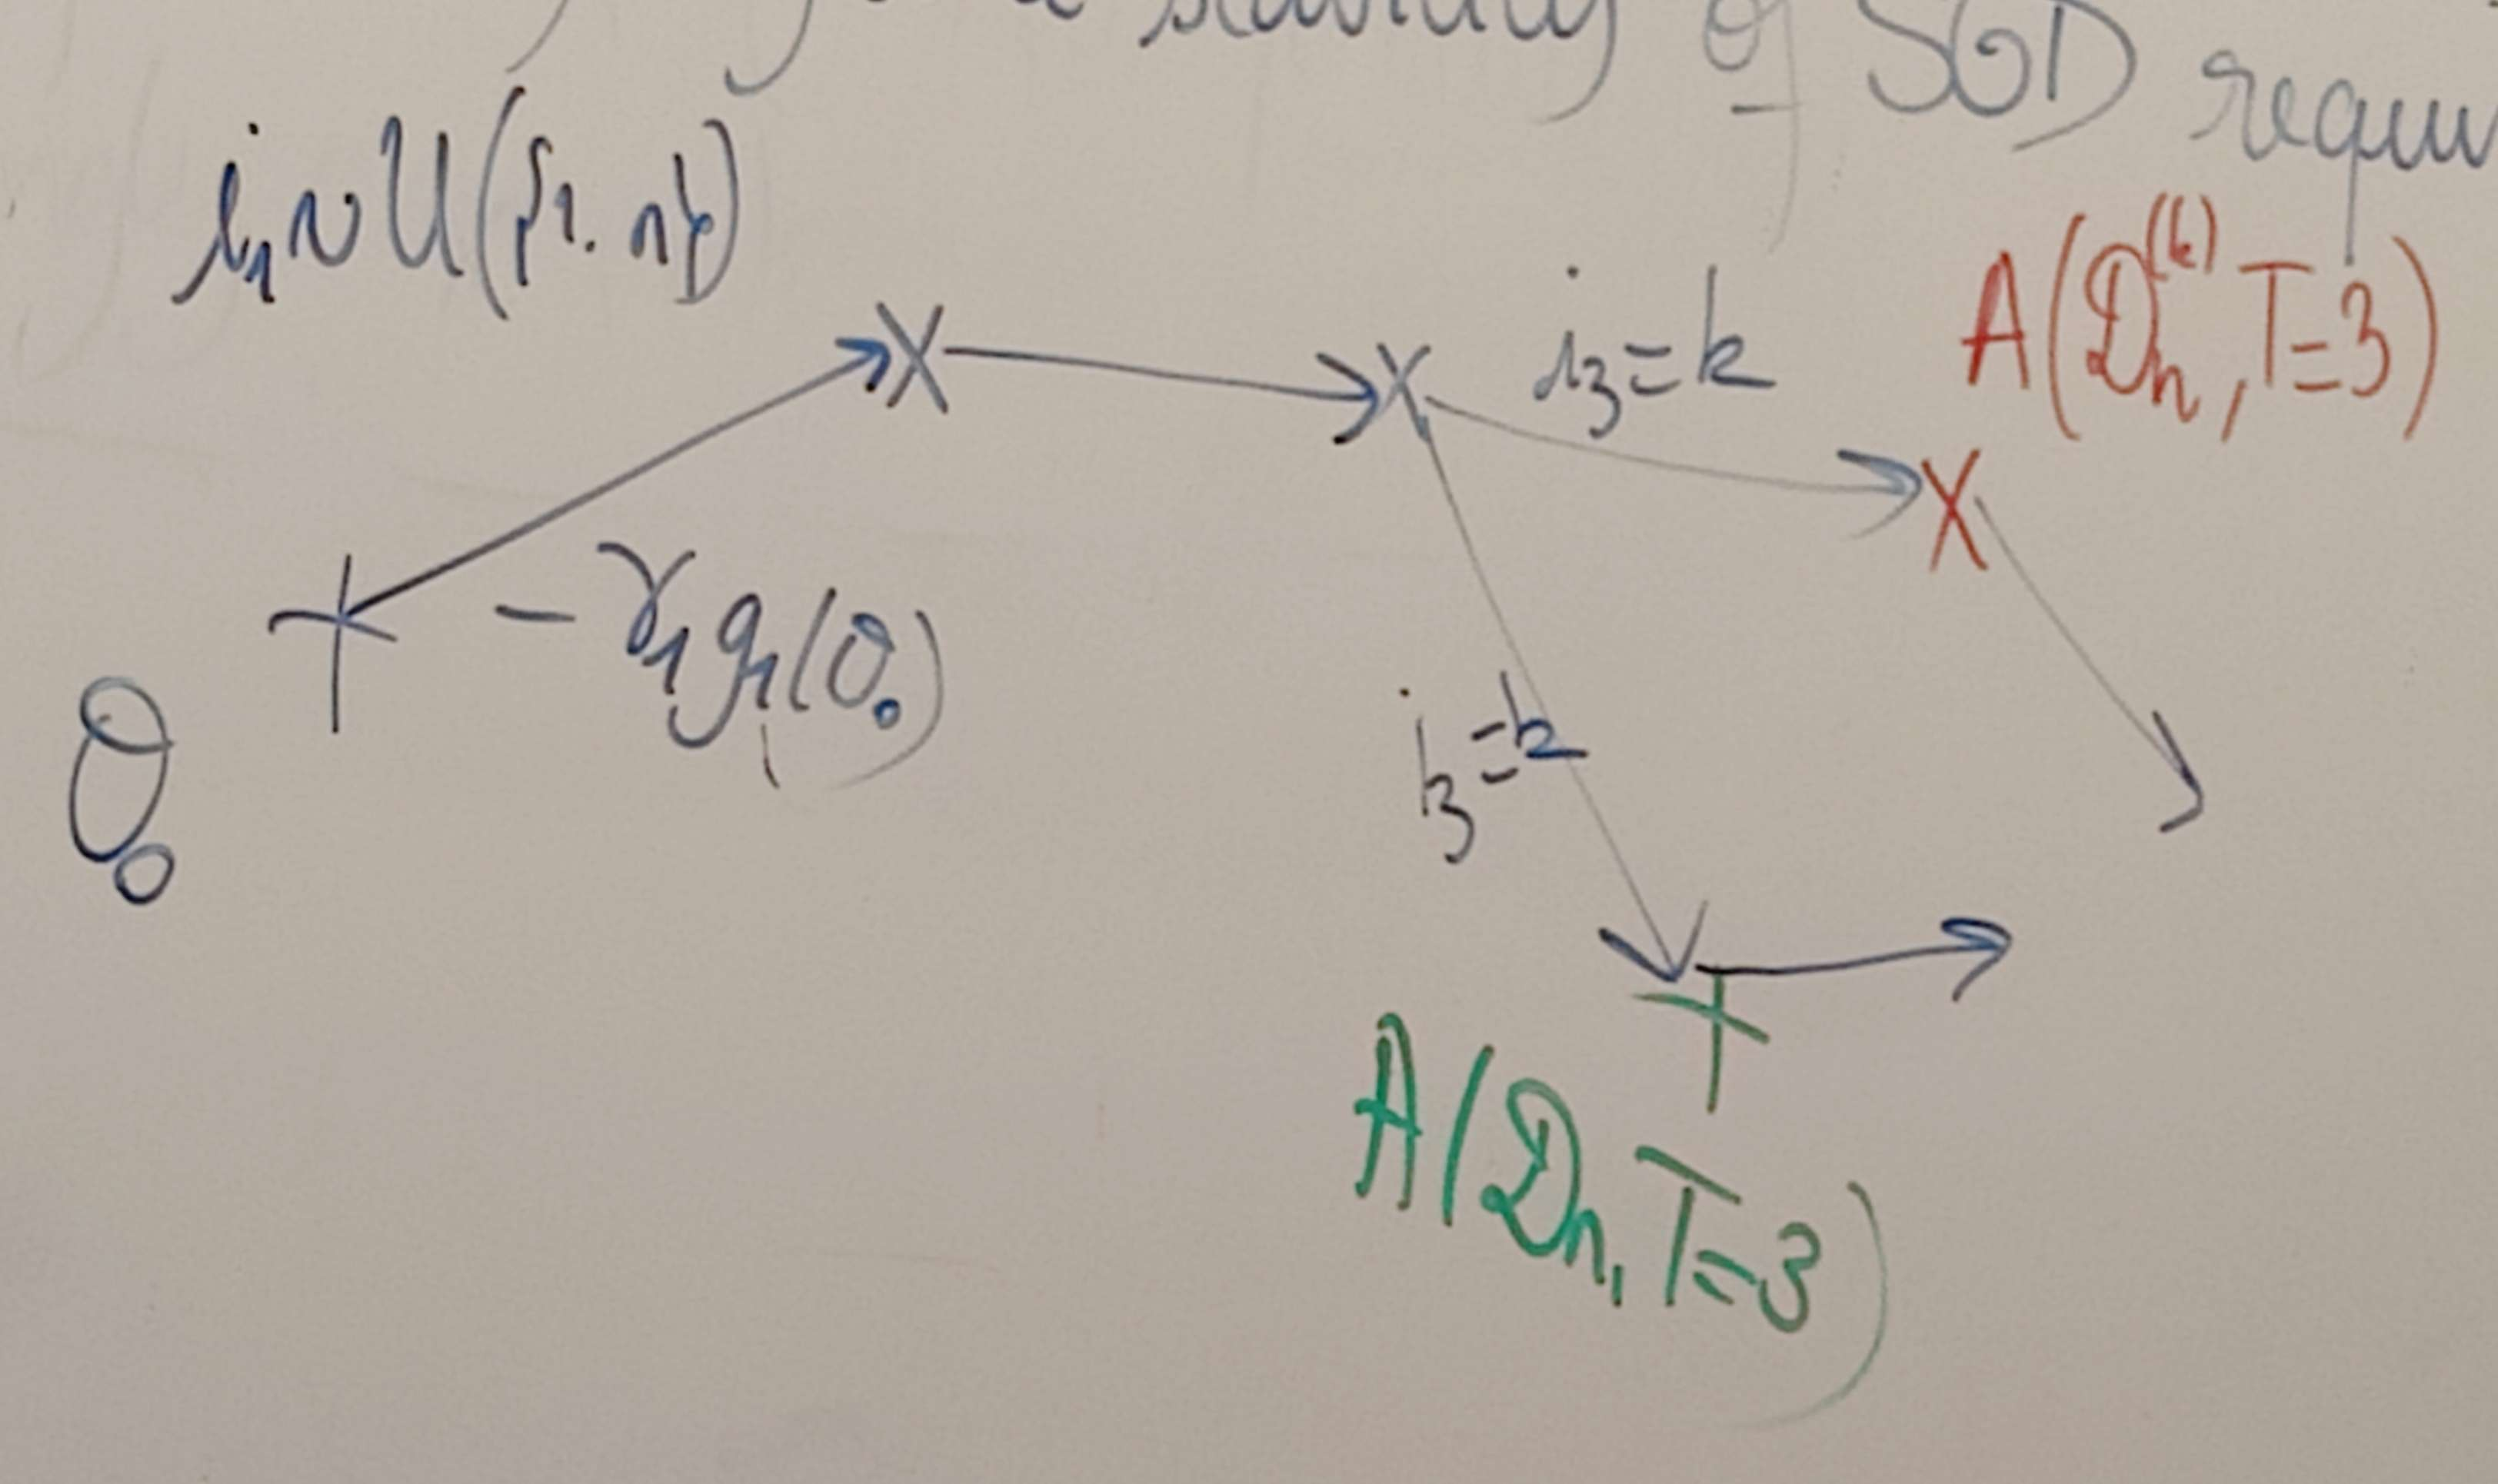
\includegraphics[width=.65\textwidth]{figs/graph.jpg}
    \caption{Difference between $A(\mathcal{D}_n)$ vs $A(\mathcal{D}_n)^{(k)}$}
\end{figure}

\textbf{goal} Control $A(\mathcal{D}_n, T_{\text{steps}}) - A(\mathcal{D}_n^{(k)}, T_{\text{steps}})$ where
\begin{itemize}
    \item for most of the steps with $\mathbb{P} = \frac{n-1}{n}$,I use the same gradients $(g_{i_t})$, $i_t \neq k$ (at different points)
    \item for some steps with $\mathbb{P} = \frac{1}{n}$, I use $g_k$ for $A(\mathcal{D}_n)$ and $g'_k$ for $A(\mathcal{D}_n^{(k)})$
\end{itemize}


\textbf{Key argument: } for any convex and $ L $-smooth $ F $, then $ \forall \theta , \eta  $ 
\begin{align*}
    \left\| \theta - \gamma \nabla F(\theta ) - \eta  + \gamma \nabla F(\eta )  \right\| _2 ^2 
        &= \left\| \theta - \eta  \right\| _2 ^2 - 2 \gamma \left\langle \theta - \eta , \nabla F(\theta ) - \nabla F(\eta ) \right\rangle + \gamma ^2 \underbrace{\left\| \nabla F(\theta ) - \nabla F(\eta ) \right\| _2 ^2}_{\leq L \left\langle \nabla F(\theta ) - \nabla F(\eta ) , \theta - \eta  \right\rangle \text{ cocoercivite}} \\
        &\leq \left\| \theta - \eta  \right\| ^2 - \underbrace{2 \gamma (1 - \frac{\gamma L }{2 }) }_{\geq 0 \text{ if } \gamma L \leq 2 } \underbrace{\left\langle \theta  - \eta , \nabla F(\theta ) - \nabla F (\eta )  \right\rangle }_{\geq 0 \text{ when } F \text{ cvx}} \\
        (\text{ if } \gamma L \leq 2) & \leq \left\| \theta  - \eta  \right\| ^2 
\end{align*}

With stong convexity, we would get $\leq  (1 - 2 \gamma \mu (1- \frac{\gamma L}{2})) \left| \theta - \eta  \right|^2 $

\begin{thm}[]
    Consider $ A \equiv  $ Algo 2, i.e. SGD with $ T $ steps \& step size $ (\gamma _t)_{t=1,\dots,T} $. \\
    Assume that $ \forall k \in \{1, \dots, n\}, \psi : \theta \mapsto l (Y_k, X_k^T \theta ) $ is convex, L-Smooth, BR Lipschitz (which is ok for $ l $ B-Lip \& $ \left\| X  \right\| \leq R  $ a.s. ) \\
    Then A is uniformly stable with $ \beta (n) = \frac{2 B^2 R^2 \sum_{t=1 }^{T } \gamma _t }{n} $ 
\end{thm}


\begin{proof}
    We have to use \textbf{averaged} uniform stab (this is a randomized algo!)

    Notation shortcuts : \begin{itemize}
        \item A($\mathcal{D}_n$, t steps) $\equiv \theta_t$
        \item A($\mathcal{D}_n^{(k)}$, t steps) $\equiv \tilde{\theta_t}$
    \end{itemize}

    $\forall t \geq 1$,
    %\begin{align*}
    %    \mathbb{E} [ \left\| & \theta_{t+1} - \tilde{\theta_{t+1}} \right\| | \mathcal{F}_t ] \\
    %    & = \mathbb{E}[ \left\| \theta_{t+1} - \tilde{\theta_{t+1}} \right\| \mathbb{1}_{i(t+1)= k} + \left\| \theta_{t+1} - \tilde{\theta_{t+1}} \right\| \mathbb{1}_{i(t+1)\neq  k}| \mathcal{F}_t] \\
    %    & = \frac{1}{n} \mathbb{E}[ \left\| \theta_{t+1} - \tilde{\theta_{t+1}} \right\| | \mathcal{F}_t, i(t+1)= k] + \frac{n-1}{n} \mathbb{E}[ \left\| \theta_{t+1} - \tilde{\theta_{t+1}} \right\| | \mathcal{F}_t, i(t+1) \neq k]
    %\end{align*}

    \begin{itemize}
        \item Conditionally to $i(t+1) = k$ ($\mathbb{E}[ \left\| \theta_{t+1} - \tilde{\theta_{t+1}} \right\| | \mathcal{F}_t, i(t+1)= k]$) , 
        \[
            \left\| \theta_{t+1} - \tilde{\theta_{t+1}} \right\| \leq \left\| \theta_{t} - \tilde{\theta_{t}} \right\| + \gamma _t ( \left\| \nabla \psi_k (\theta _k) \right\| + \left\| \nabla \tilde{\psi_k} (\tilde{\theta _k}) \right\|)
        .\]
        $\left\| \nabla \psi_k (\theta _k) \right\| \leq BR$ \\
        $\left\| \nabla \tilde{\psi_k} (\tilde{\theta _k}) \right\| \leq BR$

        \item Conditionally to $i(t+1) \neq  k$, the non-expensivness property gives that $\left\|  \theta_{t+1} - \tilde{\theta_{t+1}} \right\| \leq \left\|  \theta_{t} - \tilde{\theta_{t}} \right\|$ \\
        Therefore,
        
        \begin{align*}
            \mathbb{E}[ \left\| \tilde{\theta_{t+1}} - \theta_{t+1} \right\| | \mathcal{F}_t] &\leq \frac{1}{n} \left\| \theta_{t} - \tilde{\theta_{t}} \right\| + \frac{n-1}{n} \left\| \theta_{t} - \tilde{\theta_{t}} \right\| \\
            & = \left\| \theta_{t} - \tilde{\theta_{t}} \right\| + \frac{\gamma _ {t+1} 2BR}{n} \\
            & \dots \\
            & \leq \left\| \theta_0 - \tilde{\theta _0} \right\|  + \frac{\sum_{u=1}^{t+1}}{n}
        \end{align*}
            
        
        As previously, we have obtained a bound on $\left\| A(\mathcal{D}_n, T steps) - A(\mathcal{D_n^{(k)}}, T steps) \right\| $ witch leads to uniform stability with $\beta (n) = \frac{2B^2R^2 \sum_{t=1}^{T}\gamma _t}{n}$

        \textbf{Conclusion} What can be said about the generalization of SGD after T steps?
        \begin{itemize}
            \item Recall that for $T \leq n$, without replacement (one pass over the data), we actually minimize the generalization risk directly : we already obtained a rate in the previous lecture. 
            \item  (Charles) for T ...
        \end{itemize}
        
        
    \end{itemize}
\end{proof}

\end{document}